% === SET DOCUMENT METADATA ===
\def\docTitle{User Documentation (User Guide)}
\def\docVersion{3.1}
\def\docDate{July 20, 2026}

% === INCLUDE REUSABLE COMPONENTS ===
% === PACKAGES ===
\documentclass[12pt,a4paper]{report}
\usepackage[utf8]{inputenc}
\usepackage[T1]{fontenc}
\usepackage{geometry}
\geometry{left=2.5cm,right=2.5cm,top=2.5cm,bottom=2.5cm,headheight=24.65pt,footskip=1.5cm}
\usepackage{graphicx}
\usepackage{xcolor}
\usepackage{fancyhdr}
\usepackage{titlesec}
\usepackage{hyperref}
\usepackage{enumitem}
\usepackage{tabularx}
\usepackage{longtable}
\usepackage{array}
\usepackage{listings}
\usepackage{float}   % For [H] placement

% === BRANDING COLOR ===
\definecolor{mooveblue}{RGB}{0, 87, 184}
\definecolor{codegray}{RGB}{240, 240, 240}

% === HEADER / FOOTER SETUP ===
\pagestyle{fancy}
\fancyhf{}
\renewcommand{\headrulewidth}{1pt}
\renewcommand{\headrule}{\hbox to\headwidth{\color{mooveblue}\leaders\hrule height \headrulewidth\hfill}}

% Footer: Page number in center, left/right text for context
\fancyfoot[C]{\thepage}
\fancyfoot[L]{\textit{Confidential - Internal Use Only}}
\fancyfoot[R]{\textit{Contains Apache 2.0 Licensed Code}}

% === SECTION STYLING ===
\titleformat{\section}{\normalfont\Large\bfseries\color{mooveblue}}{\thesection}{1em}{}
\titleformat{\subsection}{\normalfont\large\bfseries\color{mooveblue}}{\thesubsection}{1em}{}
\titleformat{\subsubsection}{\normalfont\normalsize\bfseries\color{mooveblue}}{\thesubsubsection}{1em}{}
\titleformat{\paragraph}[runin]{\normalfont\normalsize\bfseries\color{mooveblue}}{\theparagraph}{1em}{}

% === CODE LISTING STYLE ===
\lstset{
    backgroundcolor=\color{codegray},
    basicstyle=\footnotesize\ttfamily,
    breaklines=true,
    frame=single
}

% === ADDITIONAL PACKAGES ===
\usepackage{enumitem}
\usepackage{colortbl}   % added for consistency

% === FOOTER OVERRIDE ===
\fancyhead[L]{\textcolor{mooveblue}{\textbf{Moove Education Platform}}}
\fancyhead[R]{\textbf{User Guide v4.0}}

% === BEGIN DOCUMENT ===
\begin{document}

% === COVER PAGE ===
\begin{titlepage}
    \centering
    \vspace*{1cm}
    
\includegraphics[width=5cm]{../logo.png}\\[1cm]
    {\Huge \textbf{Moove Education Platform}}\\[0.5cm]
    {\Large \docTitle}\\[0.5cm]
    {\large Version \docVersion}\\[0.2cm]
    {\large \docDate}\\[1.5cm]
    
    \textbf{Prepared By:}\\
    Moove\\
    \vfill
    \textit{This product includes software from the Open edX project, licensed under Apache 2.0.}\\
    \today
\end{titlepage}

% === TABLE OF CONTENTS ===
\tableofcontents
\newpage

% === LIST OF FIGURES ===
\listoffigures
\addcontentsline{toc}{section}{List of Figures}
\newpage

% === DOCUMENT MANAGEMENT SECTION ===
\section{Document Management and Quality Assurance}

\subsection{Document Purpose}
This User Guide provides comprehensive, step‑by‑step instructions for all users of the Moove Education Platform. It is organized into three main sections: \textbf{Educator Features} (for instructors and course staff), \textbf{Learner Features} (for students), and mandatory \textbf{Security and Privacy} guidelines that every user must follow.

\subsection{Quality Assurance}
\begin{itemize}
    \item All screenshots are captured from the production environment
    \item Steps are verified against the live system
    \item Security guidelines are aligned with INSA regulations
    \item Document is reviewed quarterly and updated with each release
\end{itemize}

\subsection{Document Conventions}
\begin{itemize}
    \item \textbf{Bold text}: Indicates UI elements, buttons, and menu items
    \item \texttt{Monospace text}: Indicates URLs, commands, and code
    \item \textit{Italic text}: Indicates emphasis and important notes
\end{itemize}

\newpage
\section{Introduction}
Welcome to the Moove Education Platform. This guide provides step‑by‑step instructions for all user activities, organised into three main sections: \textbf{Educator Features} (for instructors and course staff), \textbf{Learner Features} (for students), and mandatory \textbf{Security and Privacy} guidelines that every user must follow.

Screenshots are included for clarity. All images are located in the \texttt{screenshots/} directory.

\section{Educator Features}
This section covers all features available to course instructors and staff.

\subsection{Course Creation \& Planning}

\subsubsection{Create a New Course (UFR-OE-001-01)}
\begin{enumerate}
    \item Log in to the CMS (Course Management System) at \texttt{studio.educationvirtual.net}.
    \item Click the \textbf{New Course} button.
    \item Fill in the following fields:
    \begin{itemize}
        \item \textbf{Course Title}: The full name of your course.
        \item \textbf{Organization Code}: A short code for your institution (e.g., "MOOVE").
        \item \textbf{Course Number}: A unique identifier for the course (e.g., "PHYS101").
        \item \textbf{Course Run}: The specific offering (e.g., "2026\_T1").
    \end{itemize}
    \item Set the \textbf{Start Date}, \textbf{Enrollment Start} and \textbf{Enrollment End} dates.
    \item Click \textbf{Create}. Your course skeleton is now initialized.
\end{enumerate}

\begin{figure}[H]
\centering
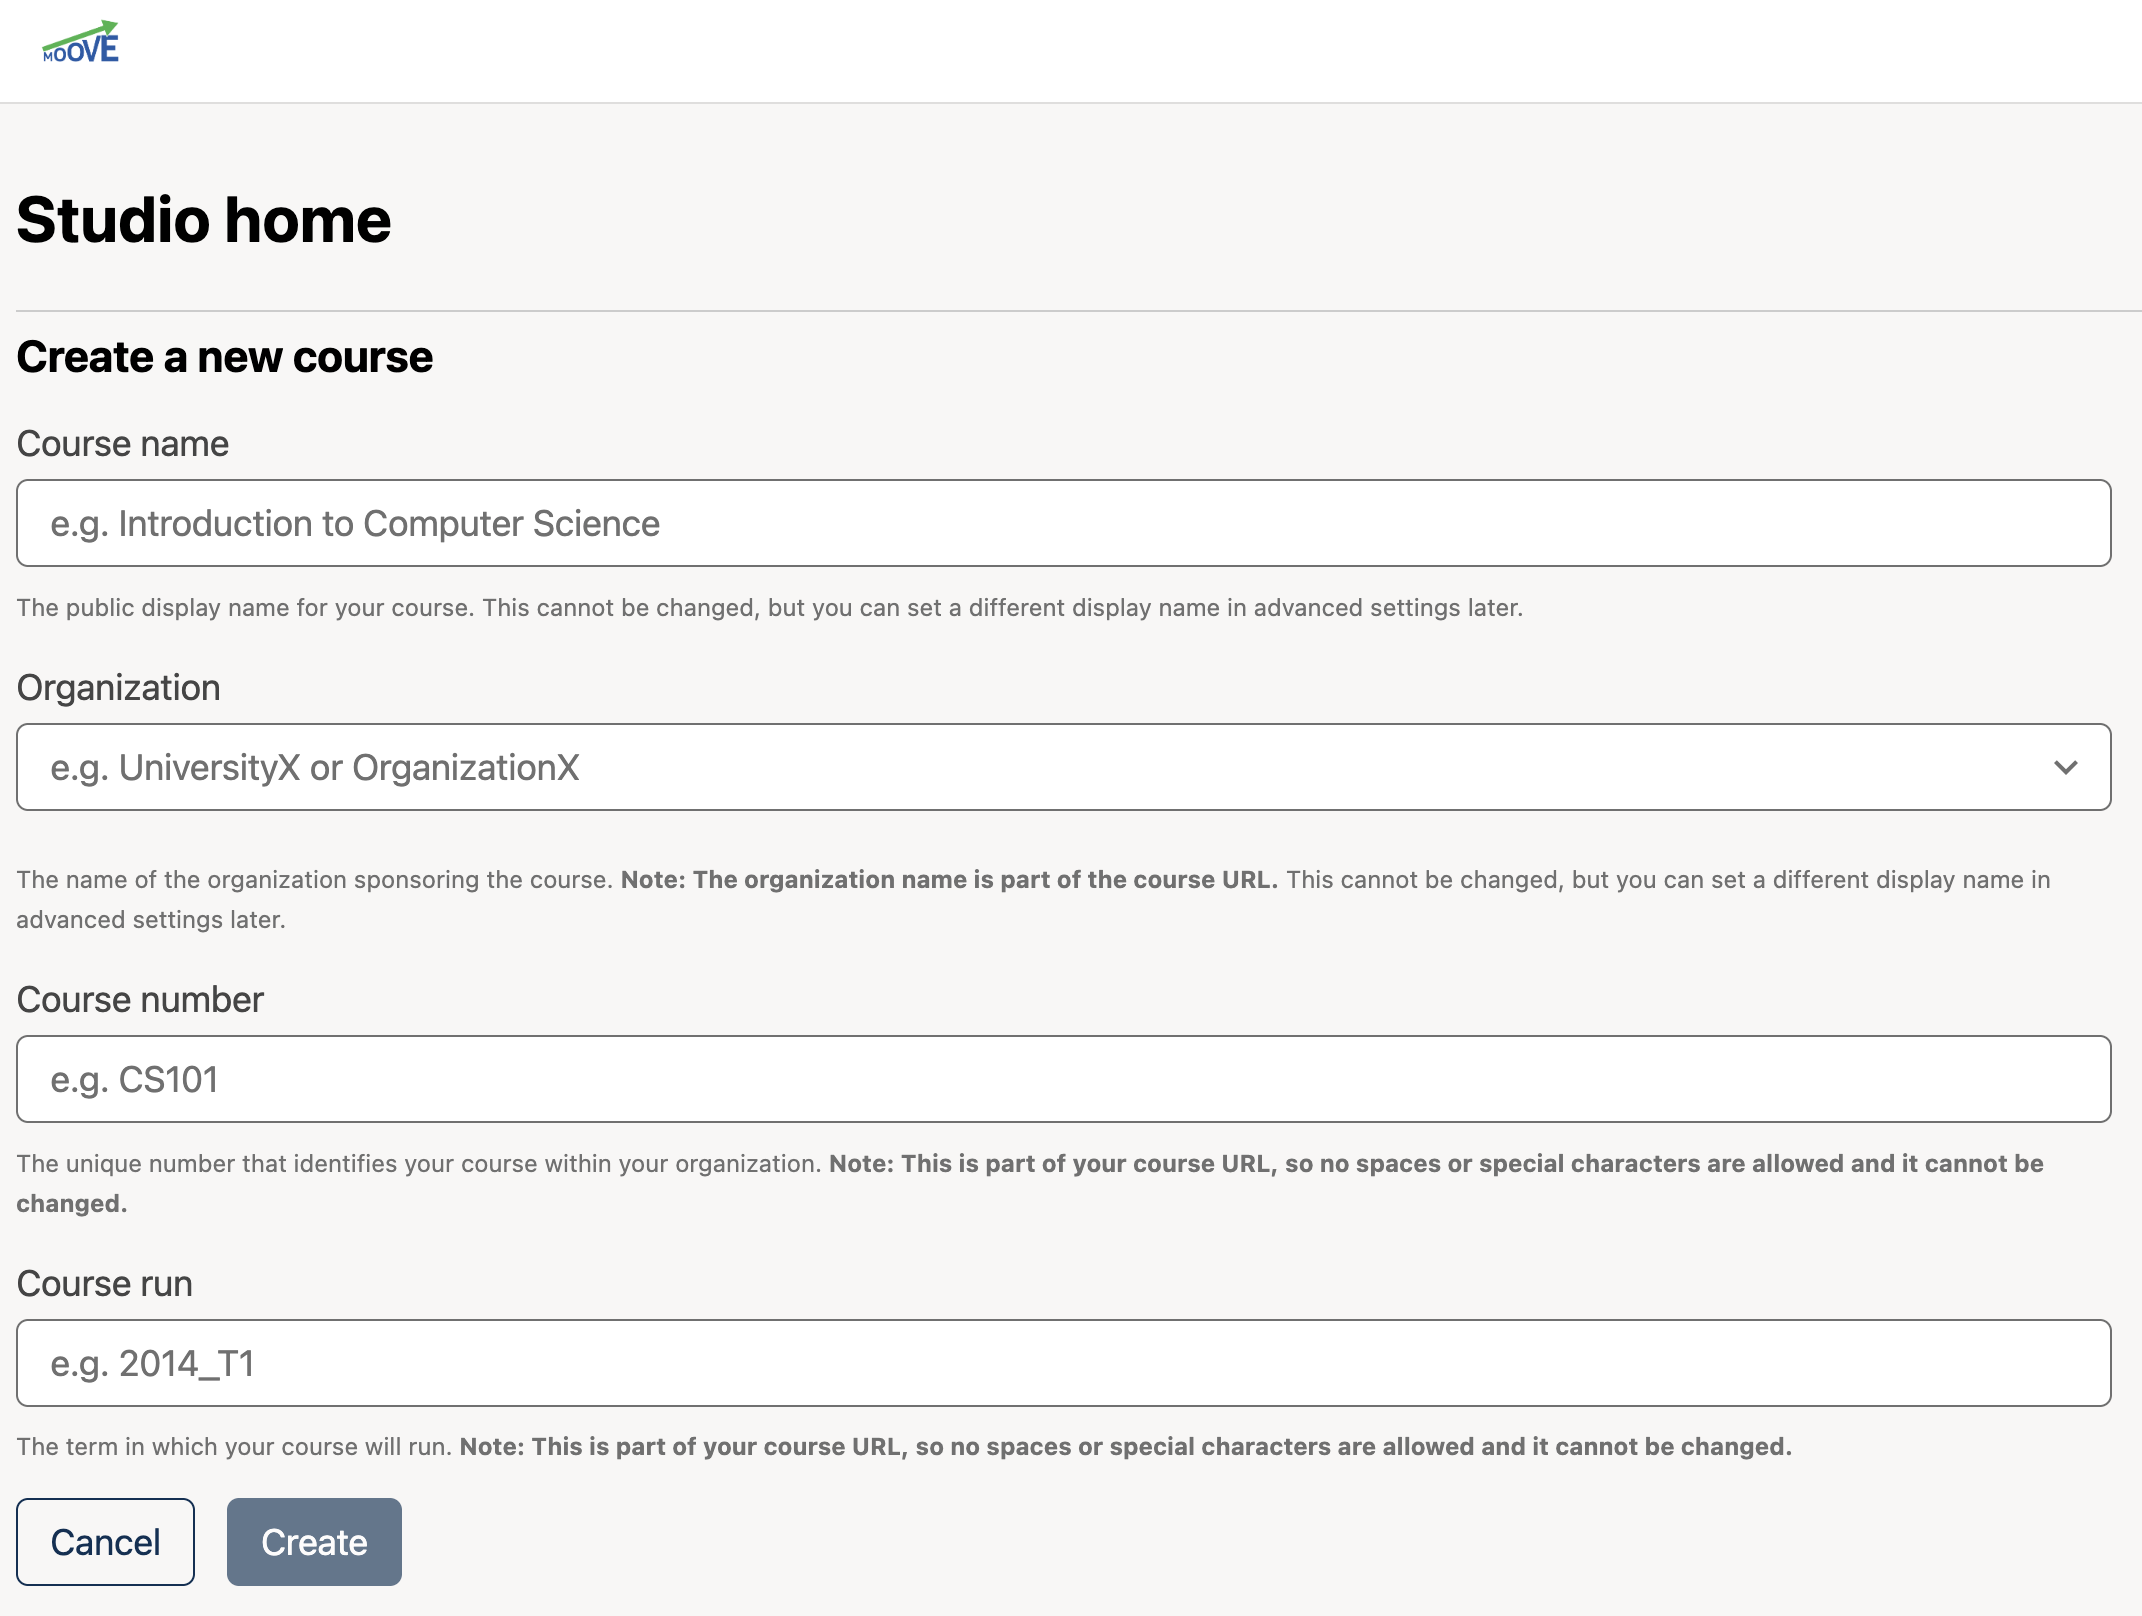
\includegraphics[width=\textwidth,height=0.6\textheight,keepaspectratio]{screenshots/create_course.png}
\caption{Course Creation Form}
\label{fig:create-course}
\end{figure}

\subsubsection{Plan a New Course (UFR-OE-001-02)}
\begin{enumerate}
    \item From the course outline page, click \textbf{Add Section}.
    \item Enter a section name (e.g., "Week 1: Introduction").
    \item Within each section, click \textbf{Add Subsection} to create sub-units.
    \item Within each subsection, click \textbf{Add Unit} to create individual content pages.
    \item Drag and drop sections/subsections/units to reorder them.
\end{enumerate}

\begin{figure}[H]
\centering
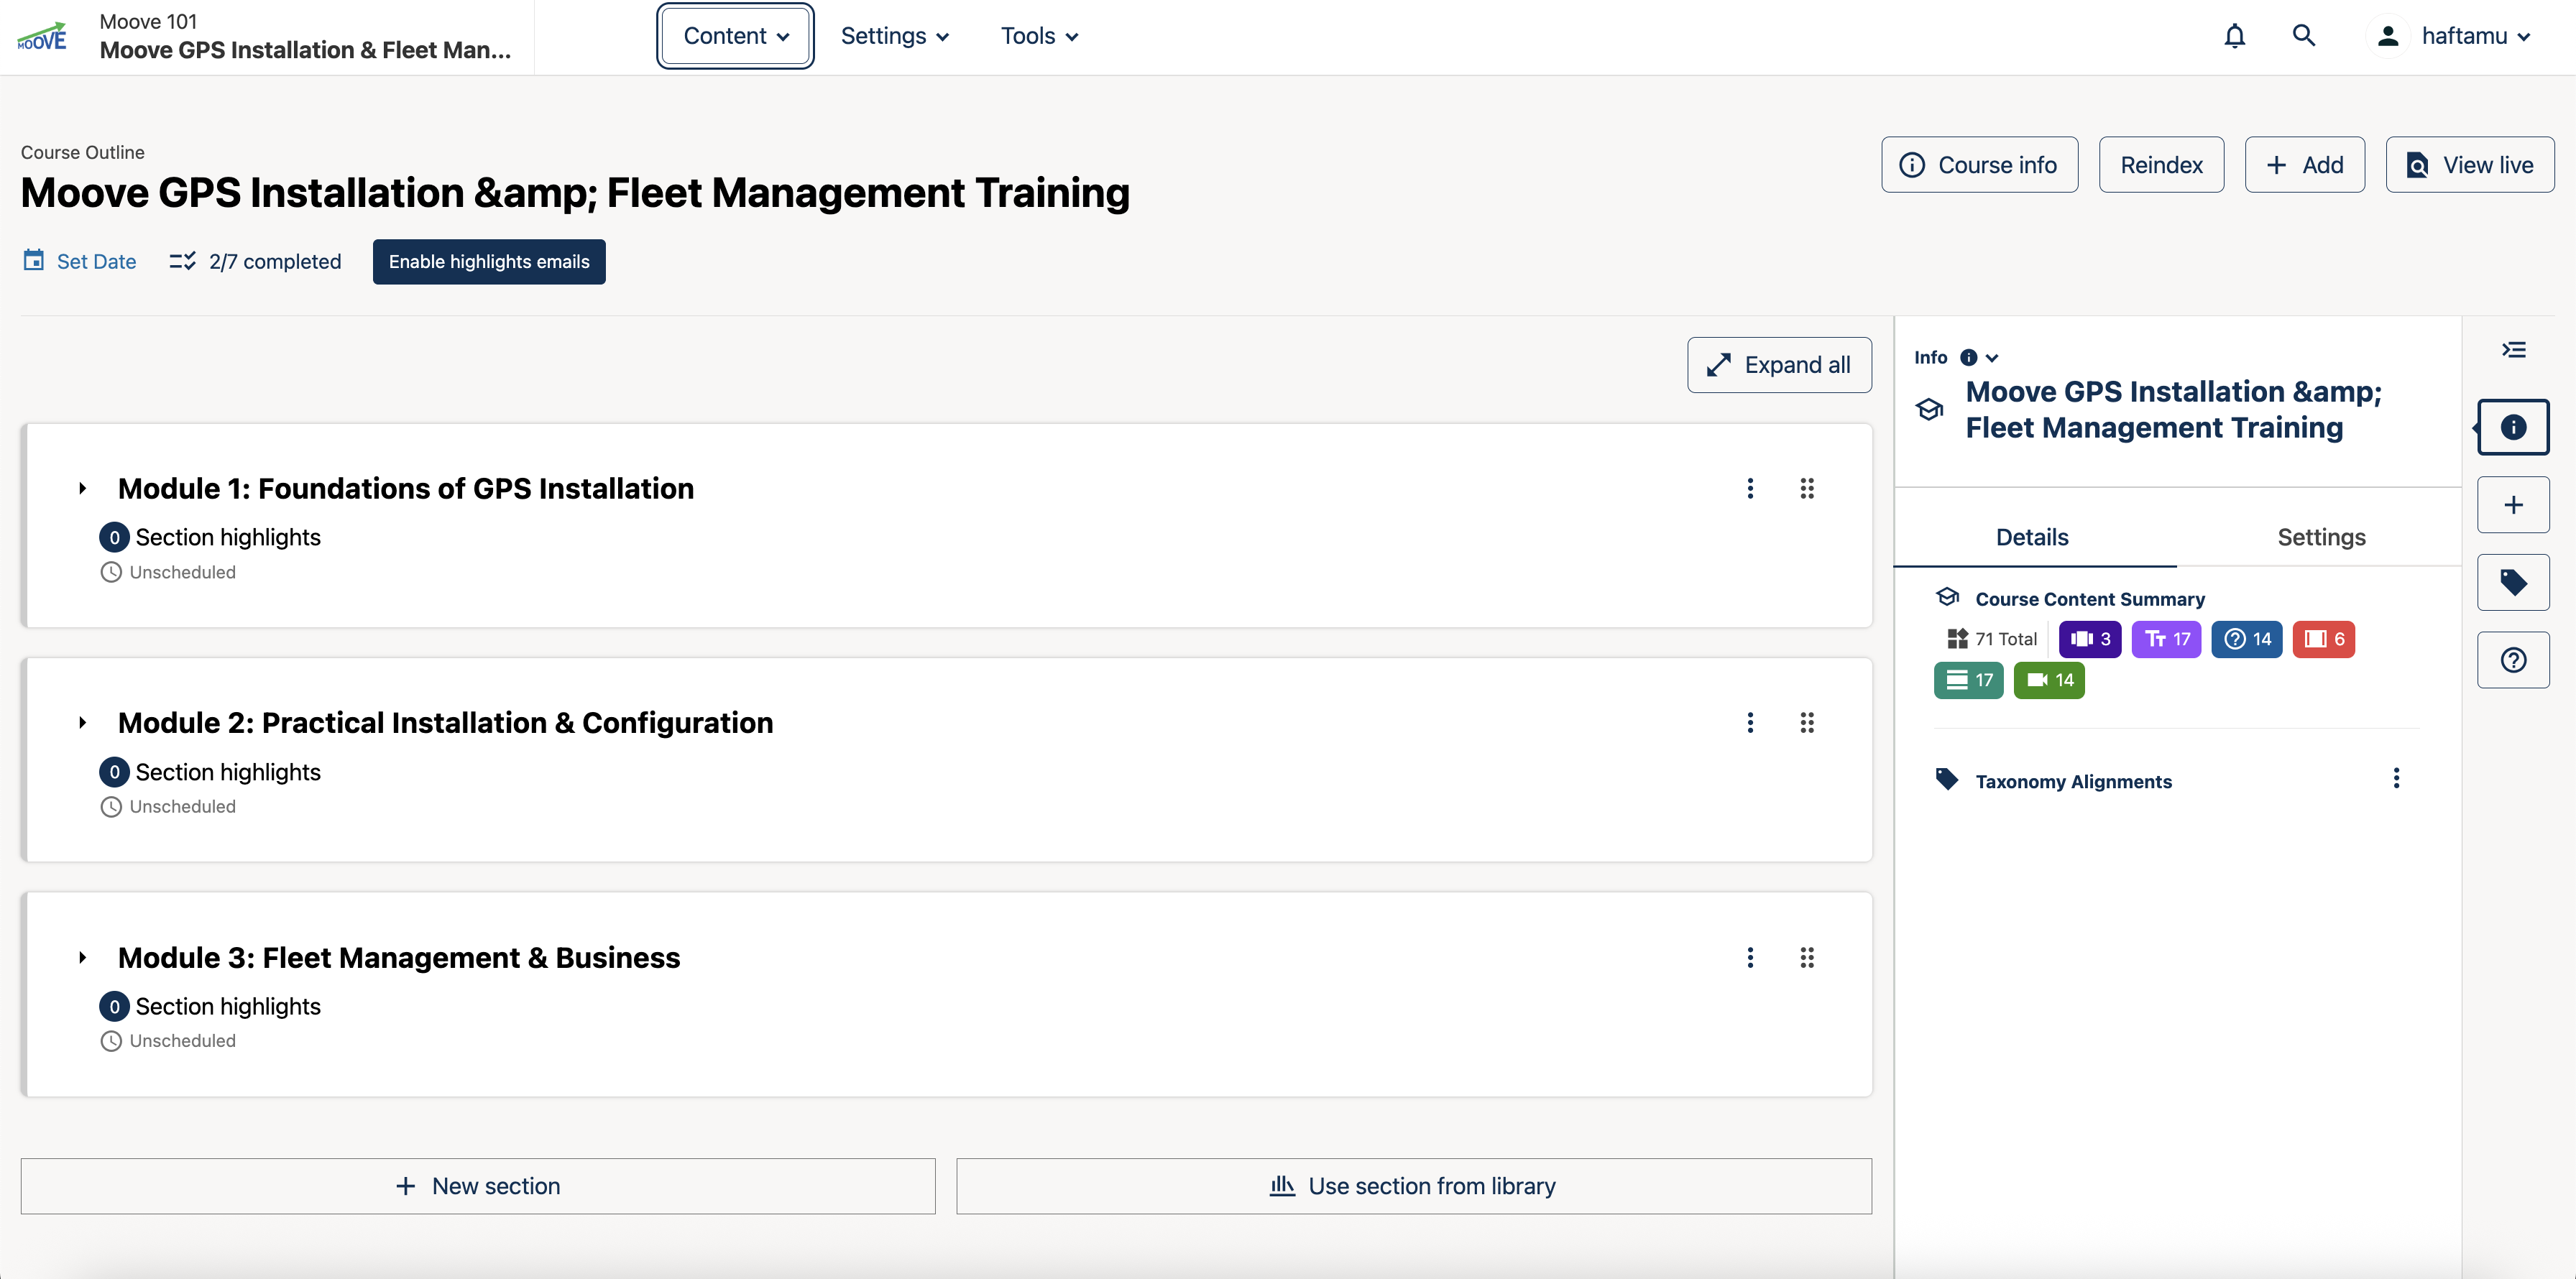
\includegraphics[width=\textwidth,height=0.6\textheight,keepaspectratio]{screenshots/course_outline.png}
\caption{Course Outline View}
\label{fig:course-outline}
\end{figure}

\subsubsection{Enroll Learners in a Course (UFR-OE-001-03)}
\begin{enumerate}
    \item Navigate to the course's \textbf{Instructor Dashboard}.
    \item Select \textbf{Enrollment} from the sidebar.
    \item To enroll individual learners: enter their email address and click \textbf{Enroll}.
    \item To bulk enroll: click \textbf{Upload CSV}, select your CSV file, and click \textbf{Upload}.
    \item The CSV format should be: \texttt{email,enrollment\_mode} (e.g., \texttt{student@email.com,verified}).
\end{enumerate}

\begin{figure}[H]
\centering
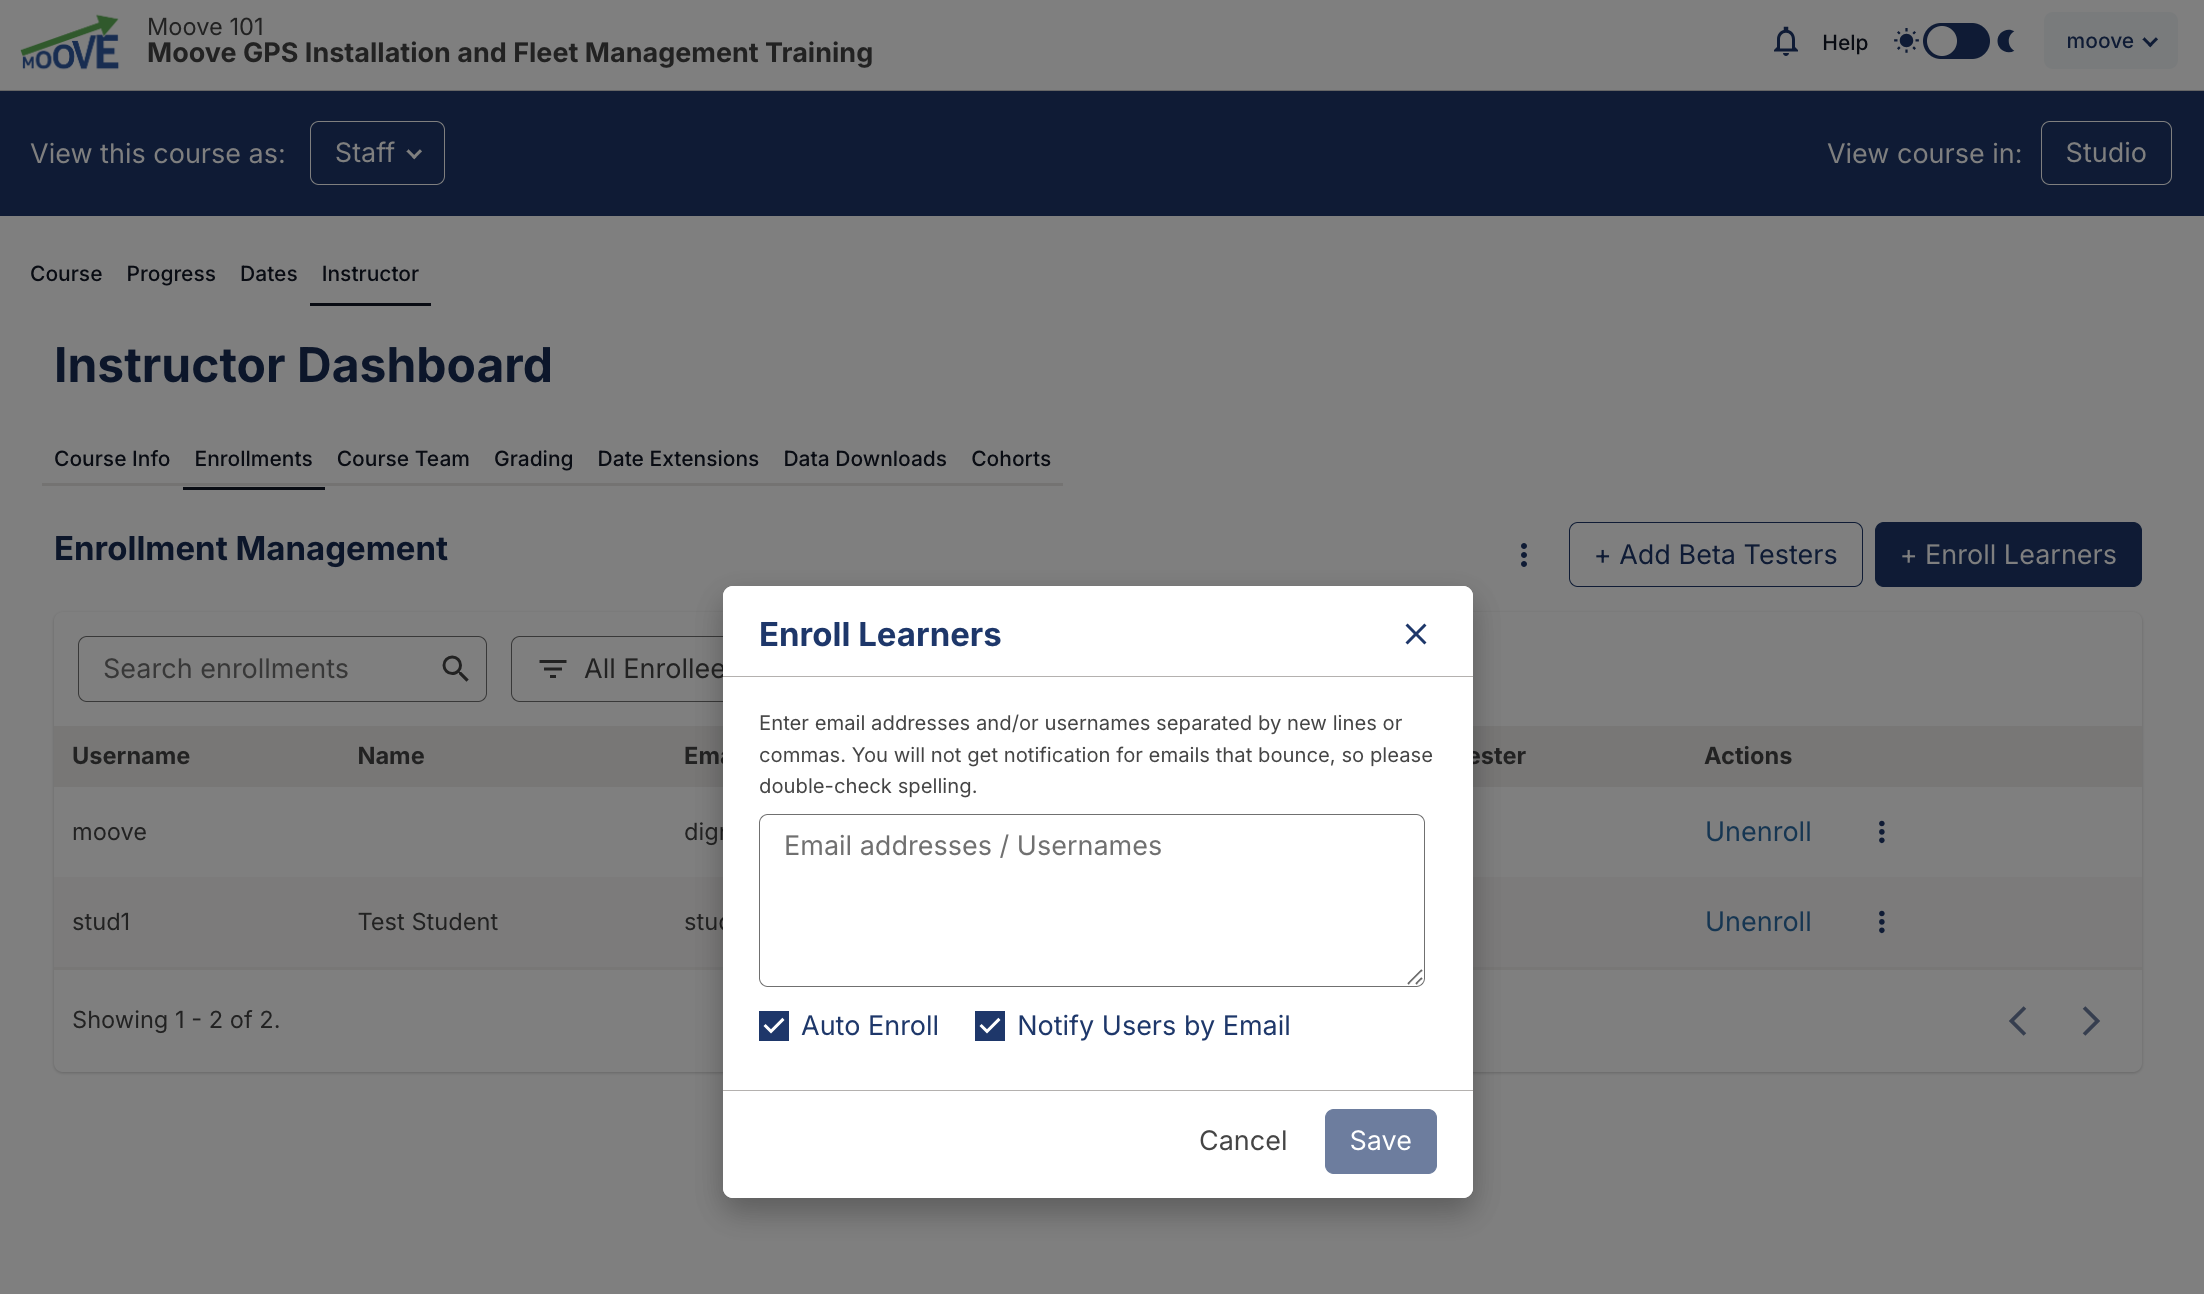
\includegraphics[width=\textwidth,height=0.6\textheight,keepaspectratio]{screenshots/enroll_learners.png}
\caption{Bulk Enrollment Upload}
\label{fig:bulk-enrollment}
\end{figure}

\subsection{Instructional Design Concepts (UFR-OE-002-01)}
\begin{itemize}
    \item Apply backward design: define learning objectives first, then create assessments, then design content.
    \item Use Bloom's Taxonomy to align assessments with learning levels.
    \item Structure your course with clear weekly modules and consistent pacing.
\end{itemize}

\subsection{Learner Engagement \& Communication}

\subsubsection{Course Discussions (UFR-OE-003-01)}
\begin{enumerate}
    \item From the course settings, navigate to \textbf{Advanced Settings}.
    \item Ensure \textbf{Enable Discussion} is set to \texttt{true}.
    \item To configure topics, go to the course outline and add a \textbf{Discussion} component.
    \item Set moderation policies in the course \textbf{Discussion Settings}.
\end{enumerate}

\begin{figure}[H]
\centering
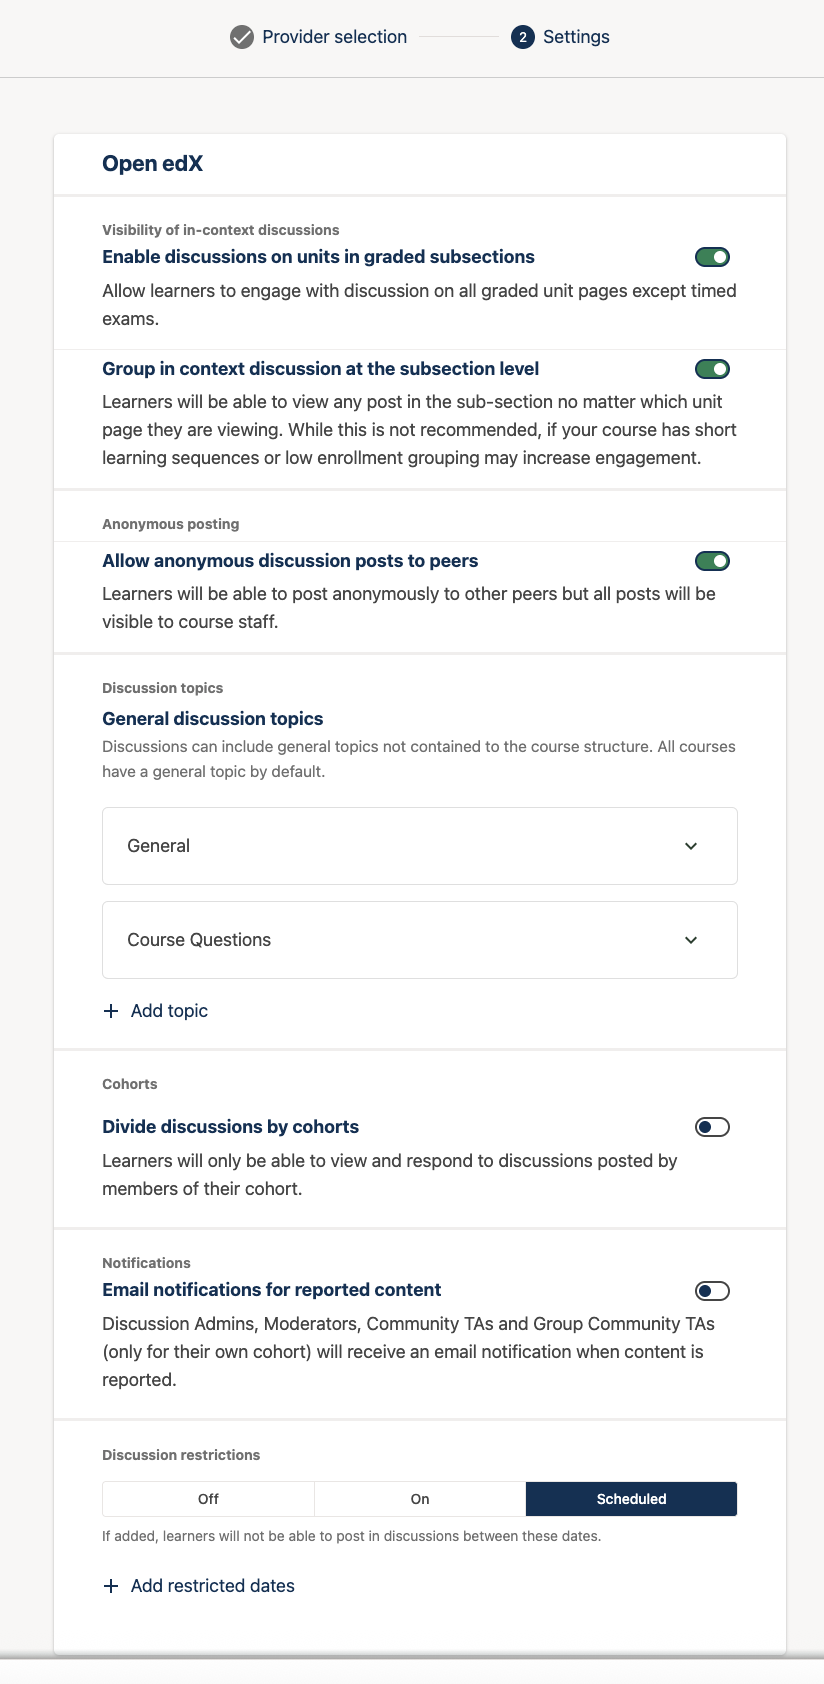
\includegraphics[width=\textwidth,height=0.6\textheight,keepaspectratio]{screenshots/discussion_settings.png}
\caption{Discussion Settings}
\label{fig:discussion-settings}
\end{figure}

\subsubsection{Bulk Emails (UFR-OE-003-02)}
\begin{enumerate}
    \item Navigate to the course \textbf{Instructor Dashboard}.
    \item Click \textbf{Email}.
    \item Select recipients:
    \begin{itemize}
        \item \textbf{All Learners}: All enrolled students.
        \item \textbf{Segments}: Filter by enrollment track, progress, or last activity.
    \end{itemize}
    \item Compose your message (supports rich text and formatting).
    \item Click \textbf{Send}. The email will be sent asynchronously.
\end{enumerate}

\begin{figure}[H]
\centering
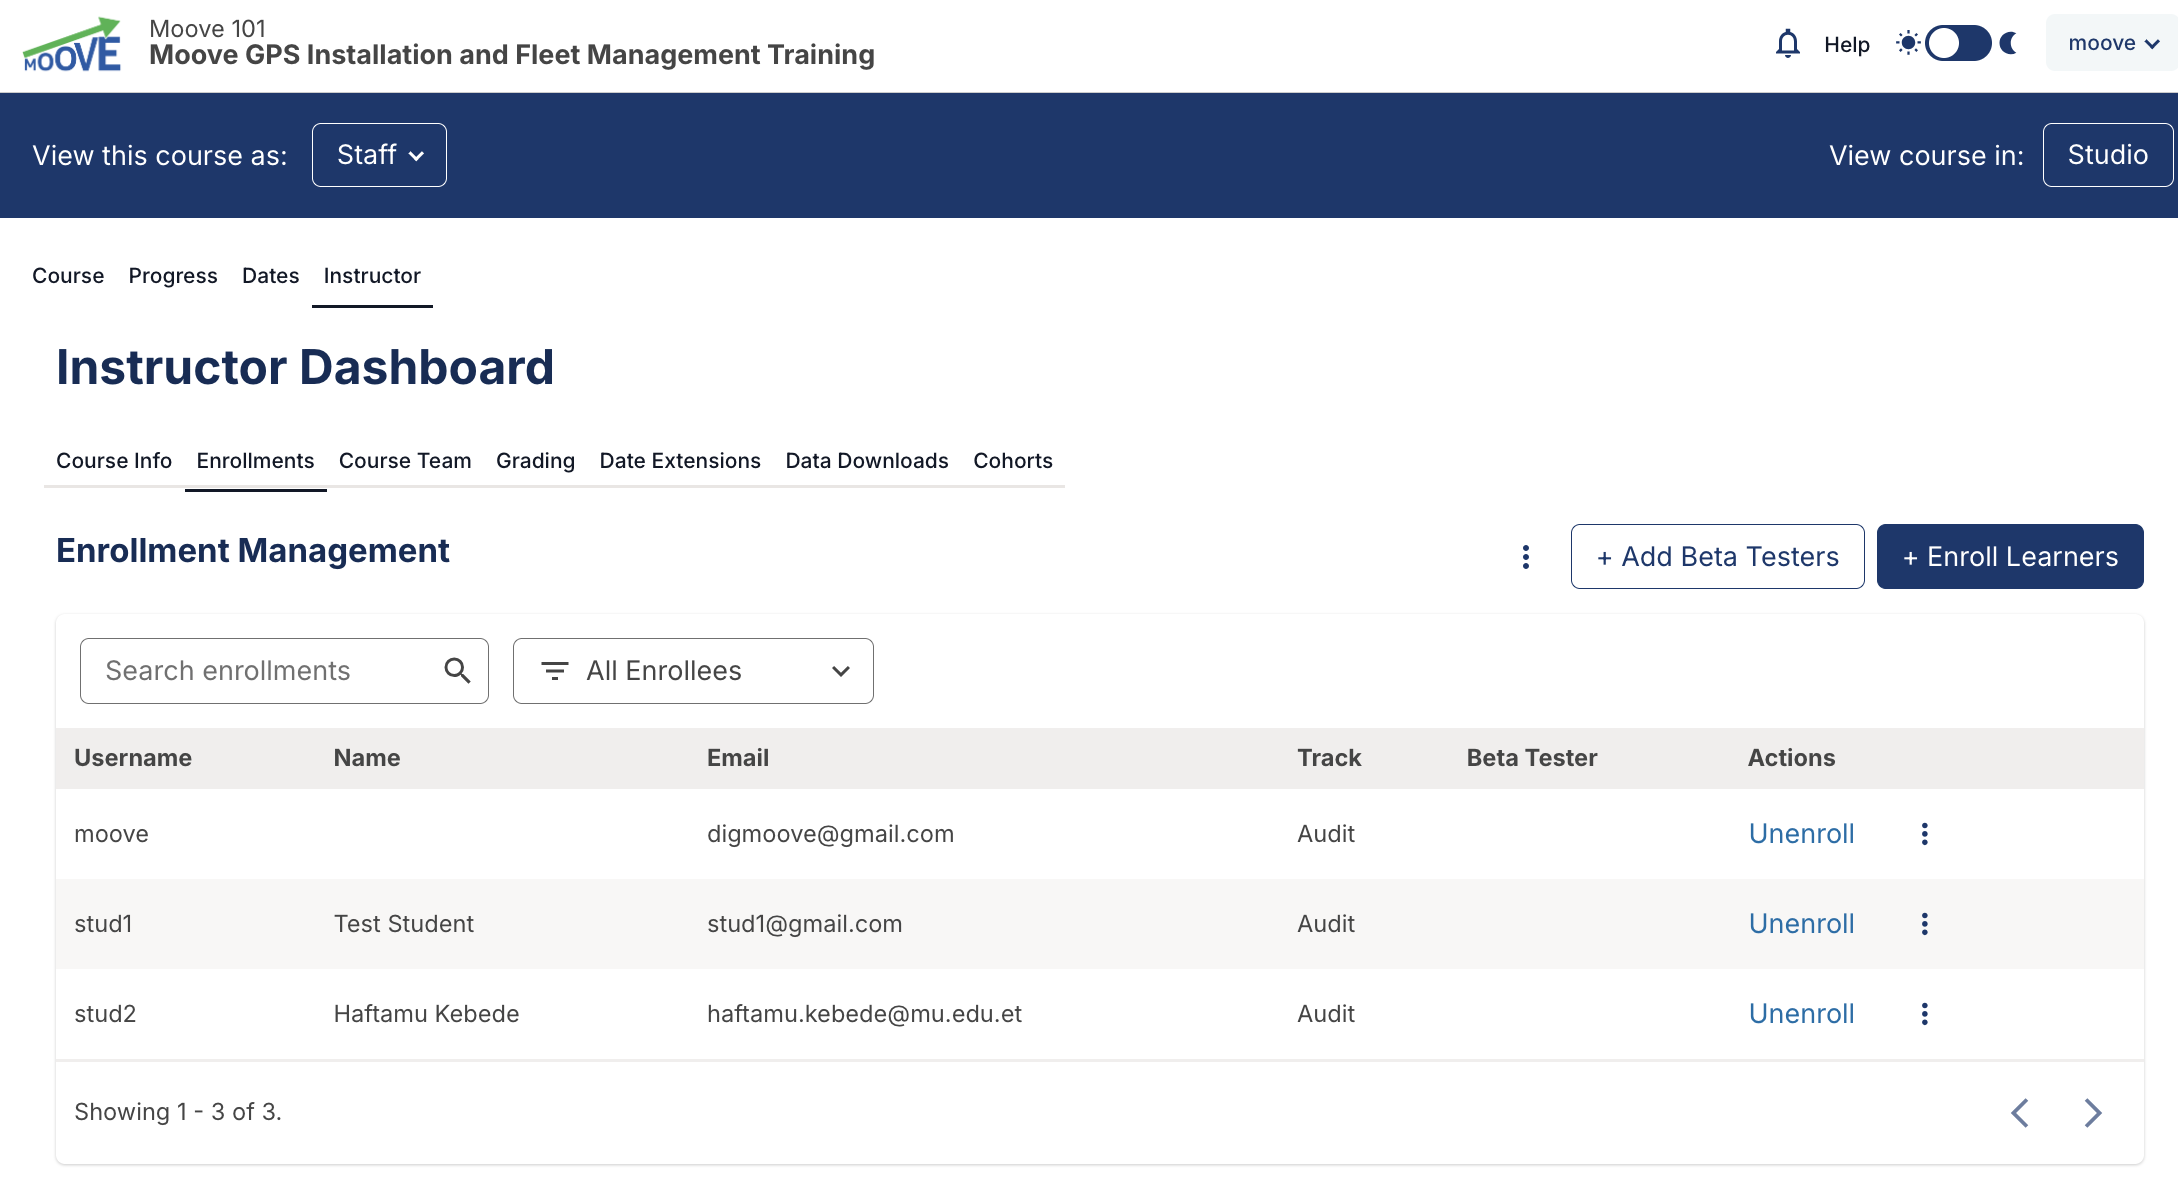
\includegraphics[width=\textwidth,height=0.6\textheight,keepaspectratio]{screenshots/bulk_email.png}
\caption{Bulk Email Composition}
\label{fig:bulk-email}
\end{figure}

\subsubsection{Course Updates (UFR-OE-003-03)}
\begin{enumerate}
    \item From the course \textbf{Instructor Dashboard}, click \textbf{Updates}.
    \item Click \textbf{Add Update}.
    \item Enter a title and content (supports rich text, images, links).
    \item Set visibility (visible to all or specific cohorts).
    \item Click \textbf{Publish}. The update will appear on the course home page.
\end{enumerate}

\begin{figure}[H]
\centering
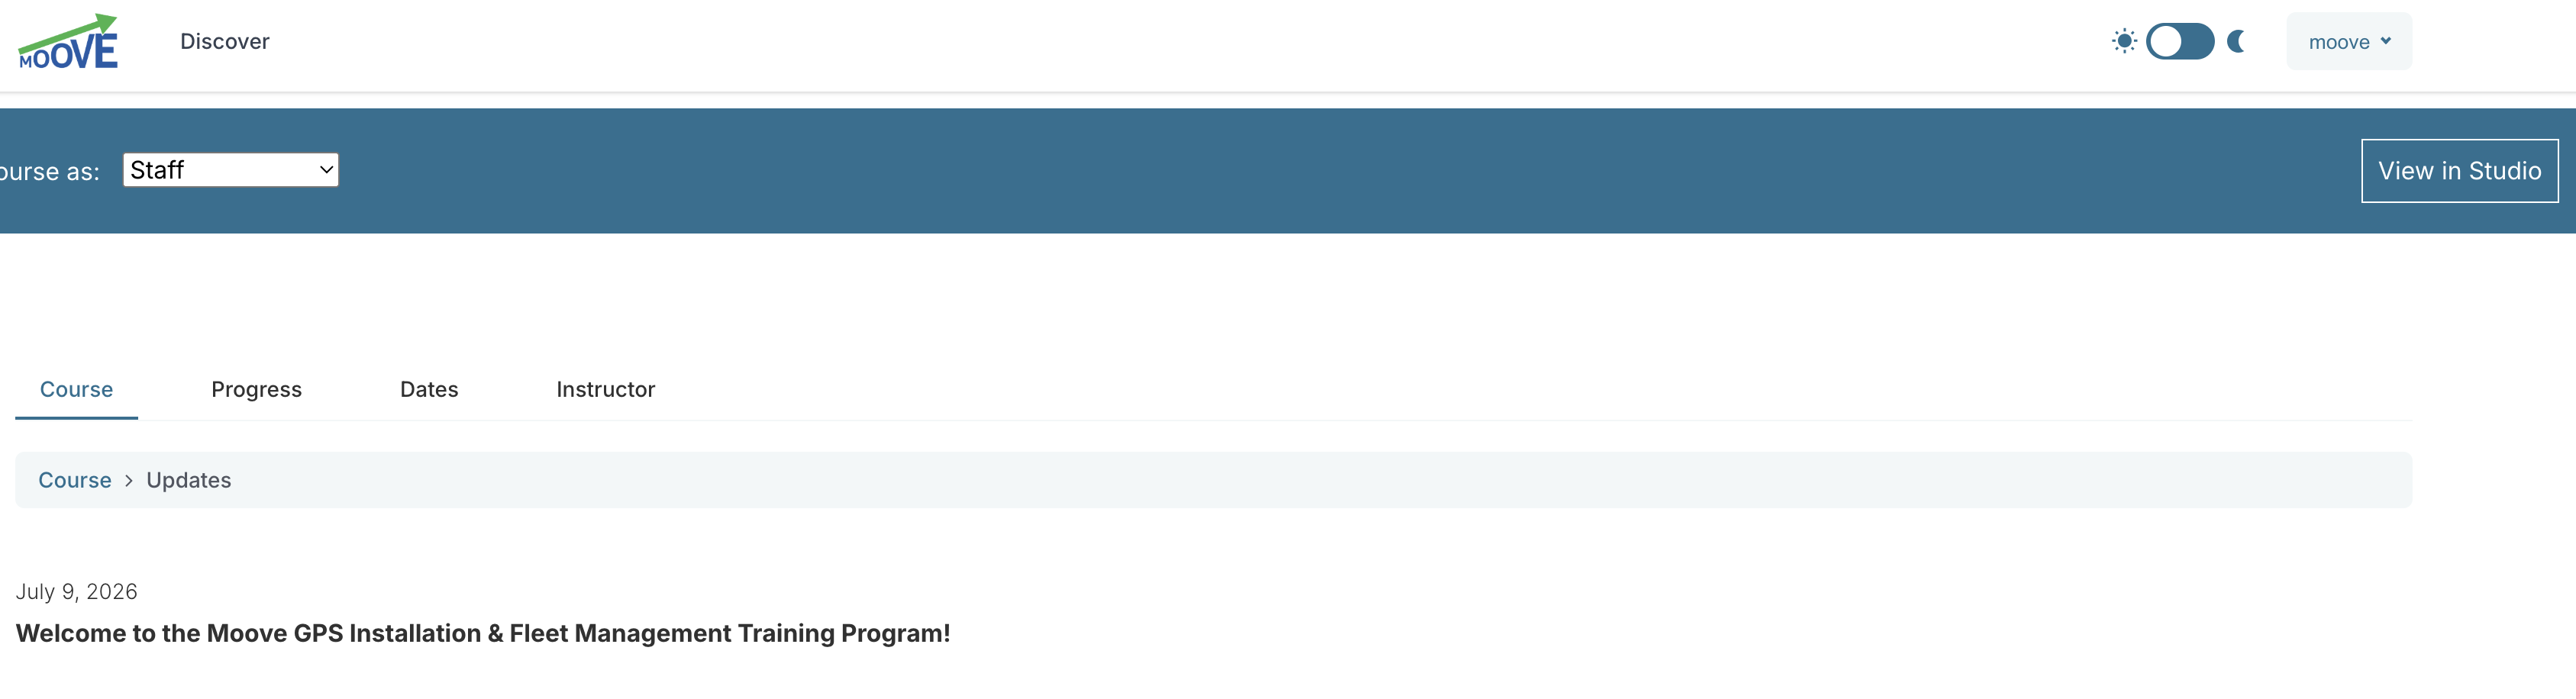
\includegraphics[width=\textwidth,height=0.6\textheight,keepaspectratio]{screenshots/course_update.png}
\caption{Course Update Form}
\label{fig:course-update}
\end{figure}

\subsection{Content Creation \& Management}

\subsubsection{Create and Manage Components (UFR-OE-004-01)}
\begin{enumerate}
    \item Navigate to a unit in your course outline.
    \item Click \textbf{Add New Component}.
    \item Select component type:
    \begin{itemize}
        \item \textbf{HTML}: Text and media content.
        \item \textbf{Video}: Video player with transcripts.
        \item \textbf{Problem}: Interactive assessments.
        \item \textbf{Discussion}: Forum thread.
        \item \textbf{Advanced}: Poll, Survey, LTI, and custom XBlocks.
    \end{itemize}
    \item Configure the component settings and save.
\end{enumerate}

\begin{figure}[H]
\centering
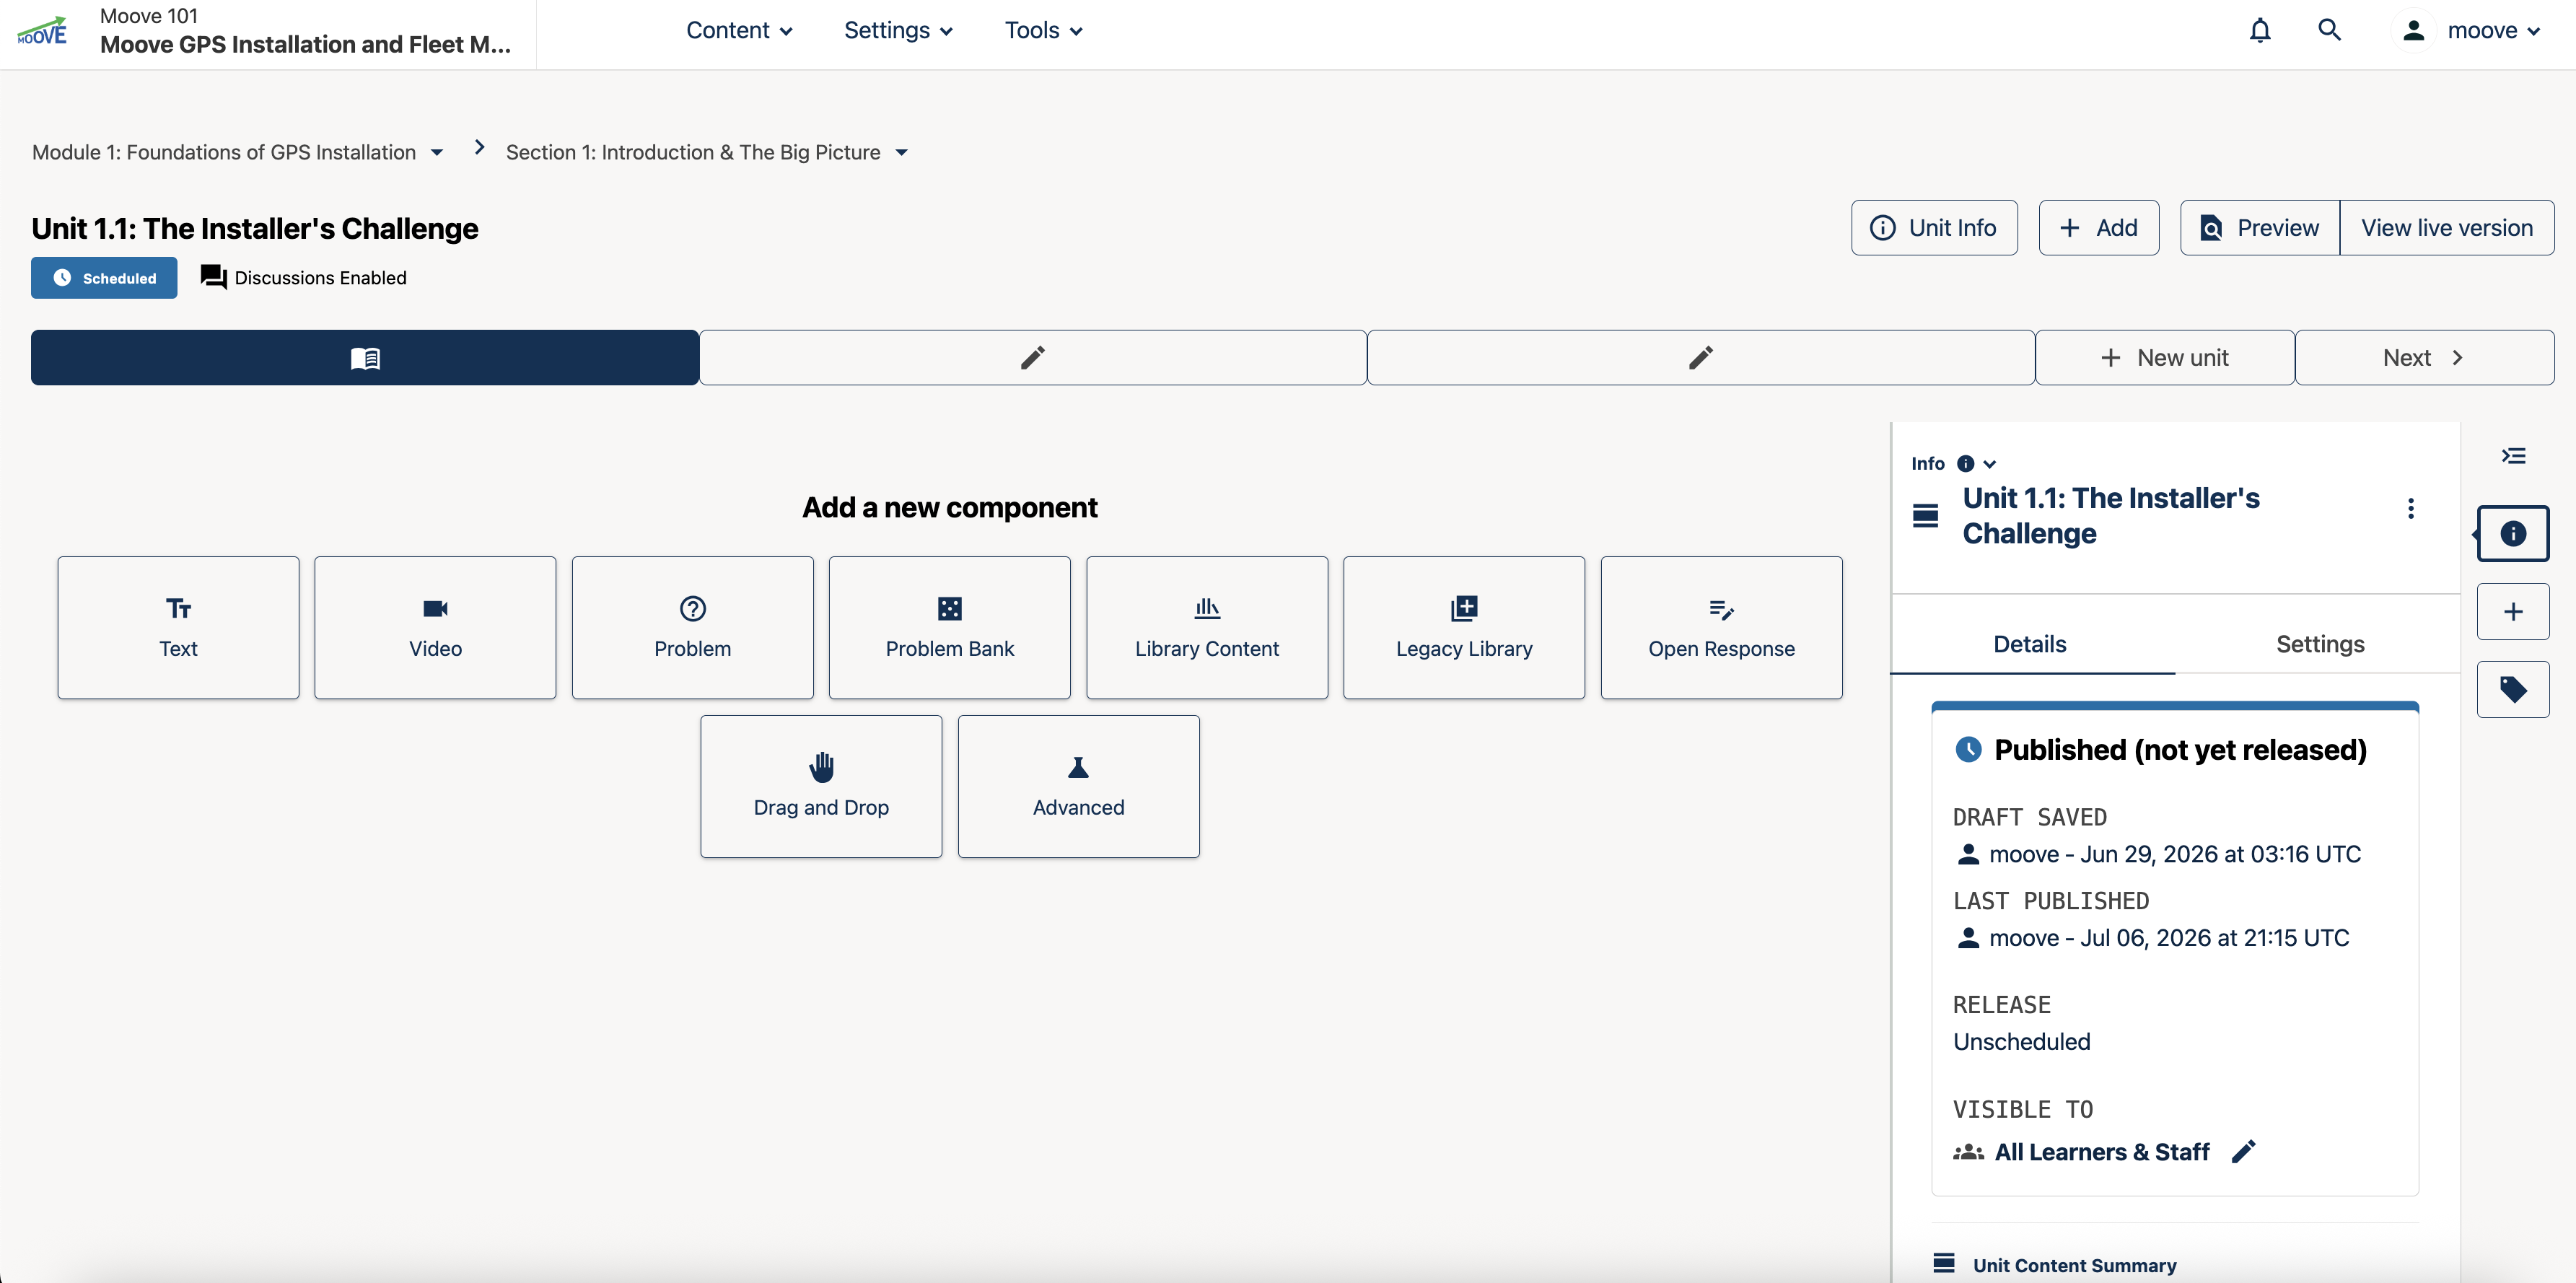
\includegraphics[width=\textwidth,height=0.6\textheight,keepaspectratio]{screenshots/add_component.png}
\caption{Add Component Dialog}
\label{fig:add-component}
\end{figure}

\subsubsection{Manage Text Components (UFR-OE-004-02)}
\begin{enumerate}
    \item Add an \textbf{HTML} component to a unit.
    \item Use the visual editor (WYSIWYG) to format text, add images, and embed media.
    \item For advanced users, click \textbf{View} or \textbf{Edit HTML} to work with raw code.
    \item LaTeX equations are supported via \texttt{\$...\$} syntax.
    \item Click \textbf{Save}.
\end{enumerate}

\begin{figure}[H]
\centering
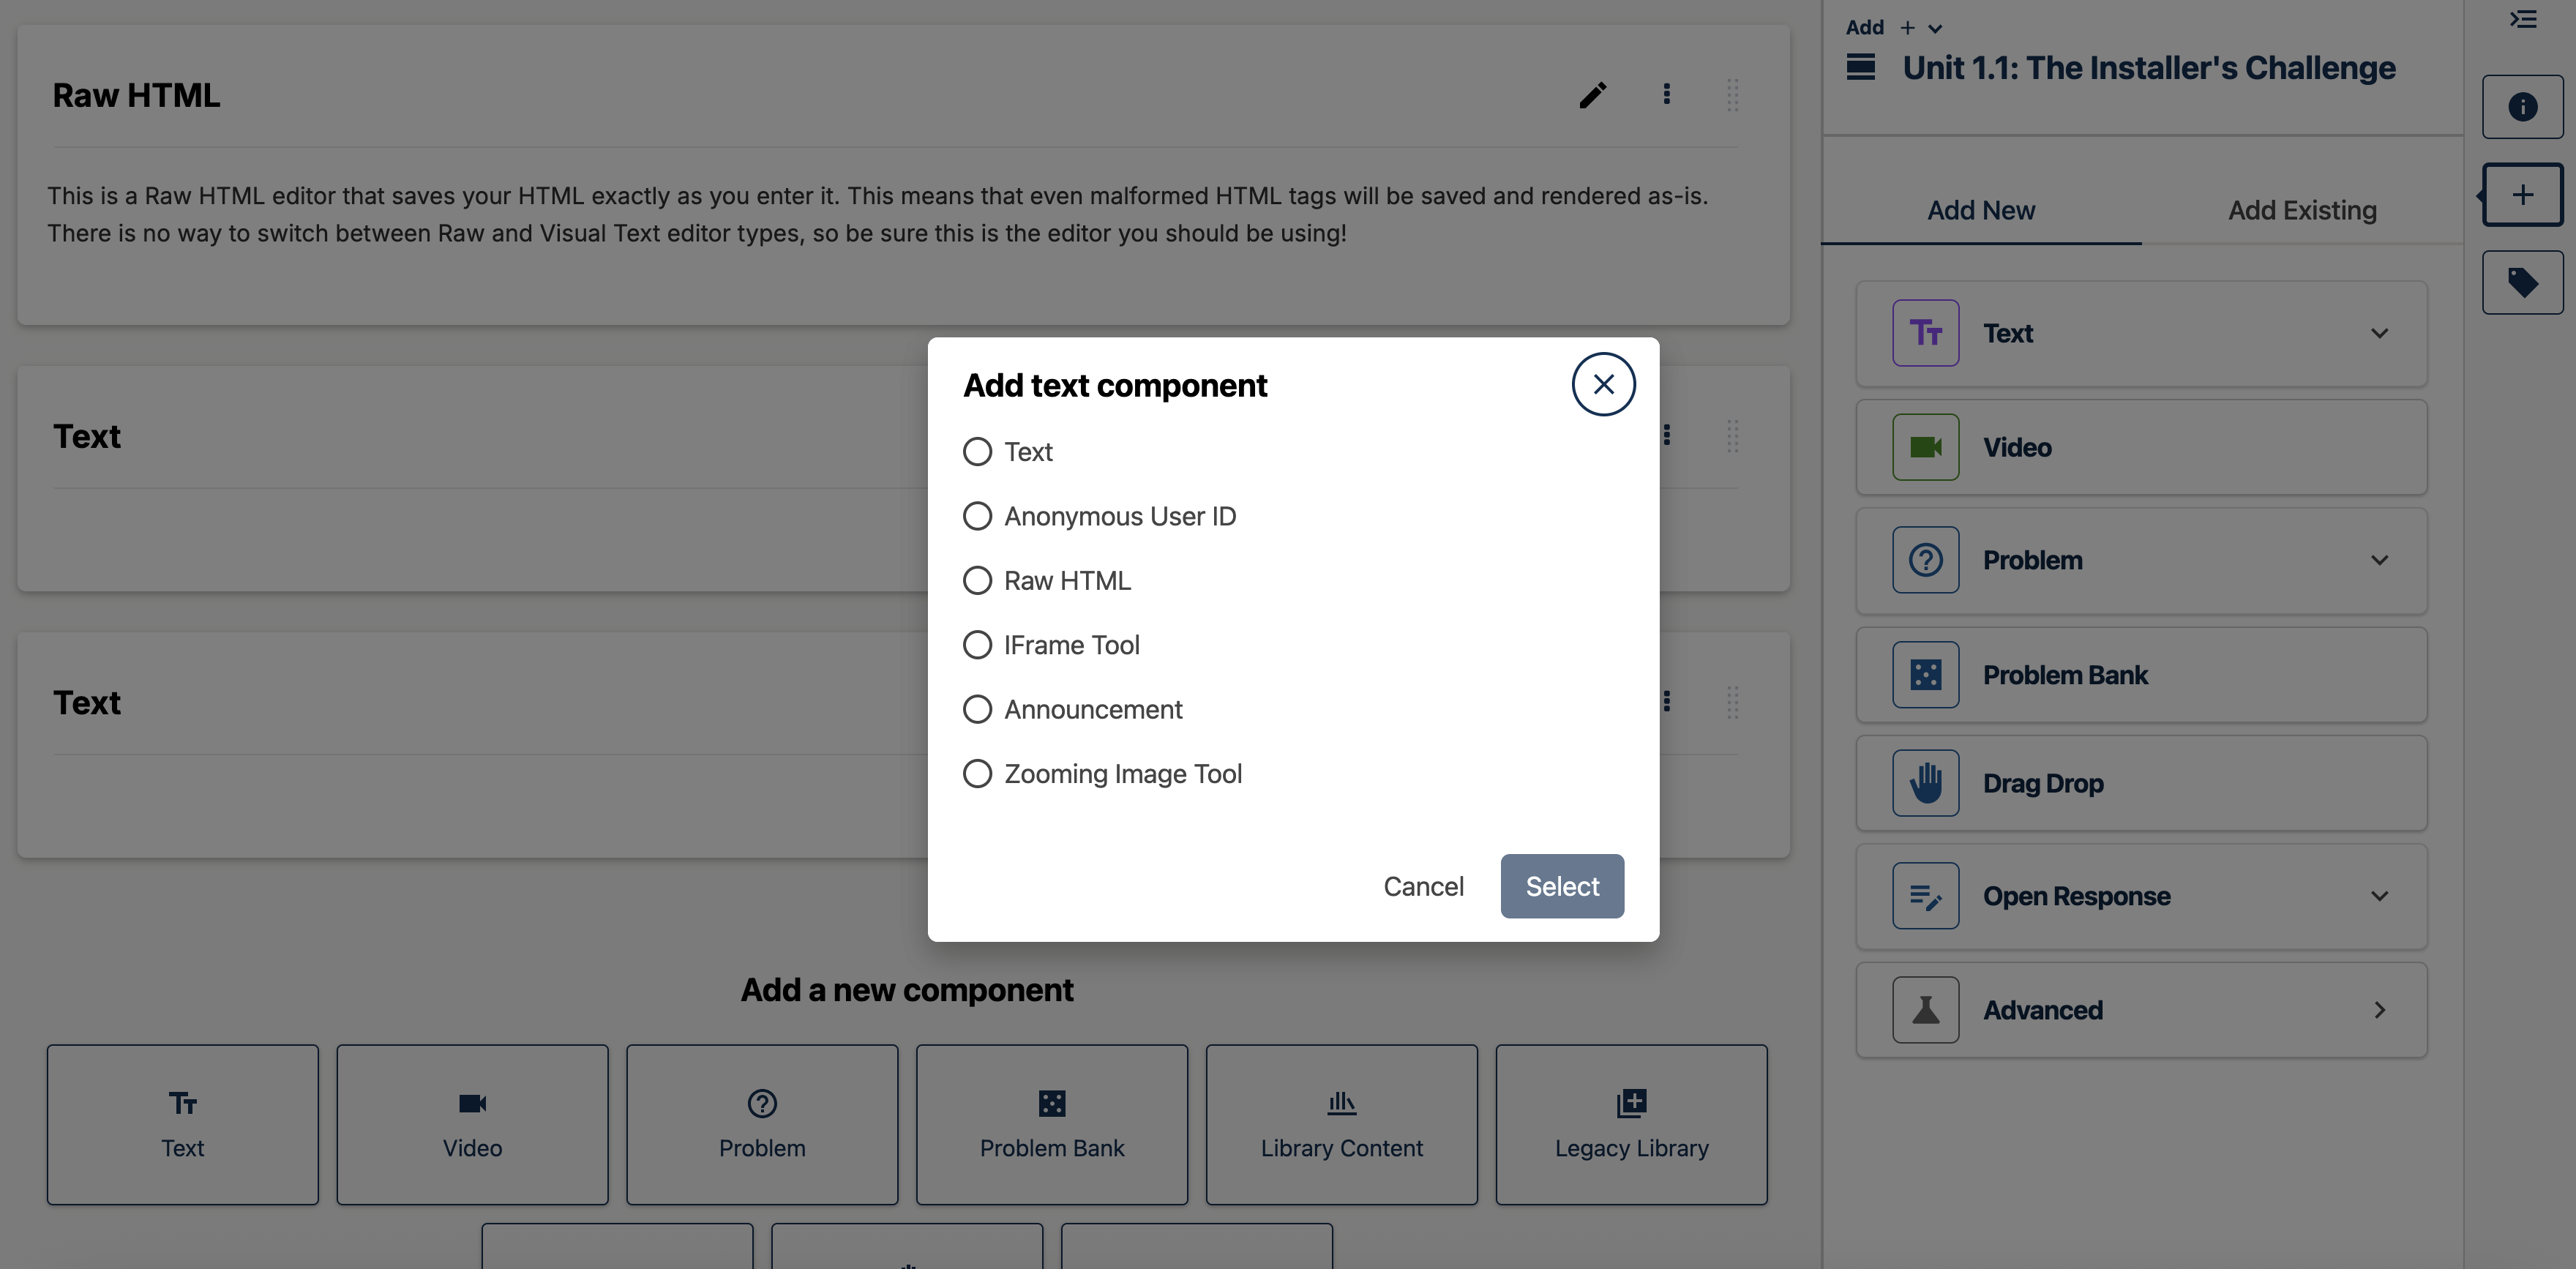
\includegraphics[width=\textwidth,height=0.6\textheight,keepaspectratio]{screenshots/html_editor.png}
\caption{HTML/Text Editor}
\label{fig:html-editor}
\end{figure}

\subsubsection{Manage Video Components (UFR-OE-004-03)}
\begin{enumerate}
    \item Add a \textbf{Video} component to a unit.
    \item Upload a video file (or enter a YouTube/Vimeo URL).
    \item The system will process and display the video player.
    \item To add a transcript:
    \begin{enumerate}
        \item Click \textbf{Upload Transcript}.
        \item Select an \texttt{.srt} or \texttt{.vtt} file.
        \item The transcript will appear as closed captions.
    \end{enumerate}
    \item Set playback options: \textbf{Downloadable}, \textbf{Speed Control}.
\end{enumerate}

\begin{figure}[H]
\centering
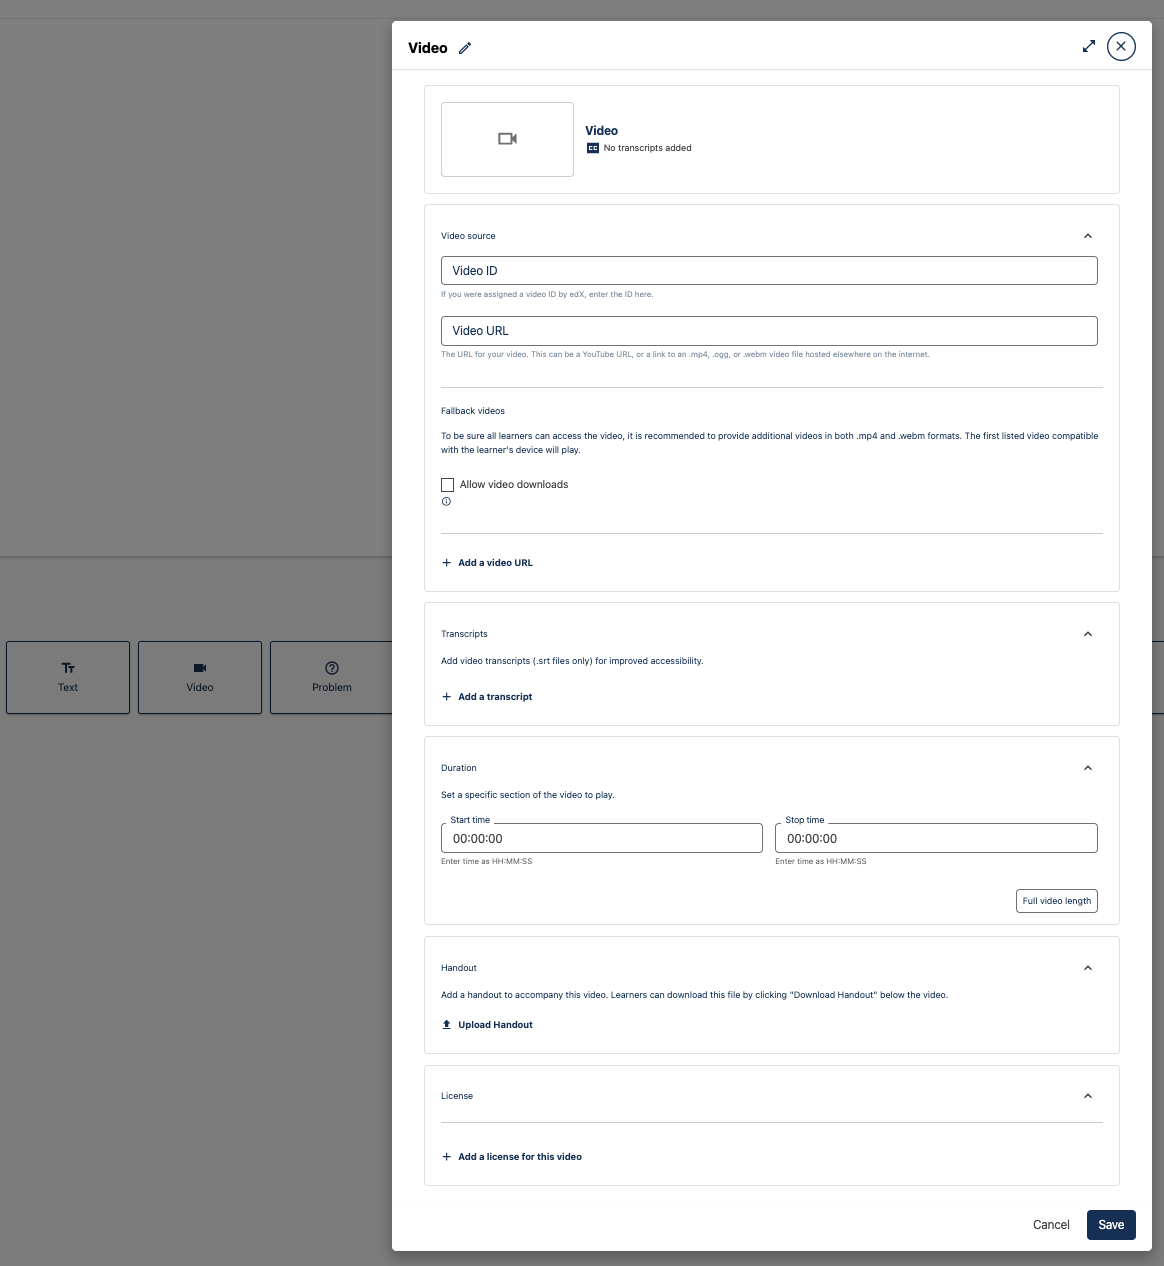
\includegraphics[width=\textwidth,height=0.6\textheight,keepaspectratio]{screenshots/video_component.png}
\caption{Video Component Editor}
\label{fig:video-component}
\end{figure}

\subsubsection{Control Content Visibility \& Access (UFR-OE-004-04)}
\begin{enumerate}
    \item For any section, subsection, or unit, open the \textbf{Settings} panel.
    \item Set \textbf{Release Date}: Content becomes visible after this date.
    \item Set \textbf{Prerequisites}: Learners must complete specific content first.
    \item Set \textbf{Visibility}: \textbf{Public} (everyone) or \textbf{Staff Only}.
    \item Click \textbf{Save}.
\end{enumerate}

\begin{figure}[H]
\centering
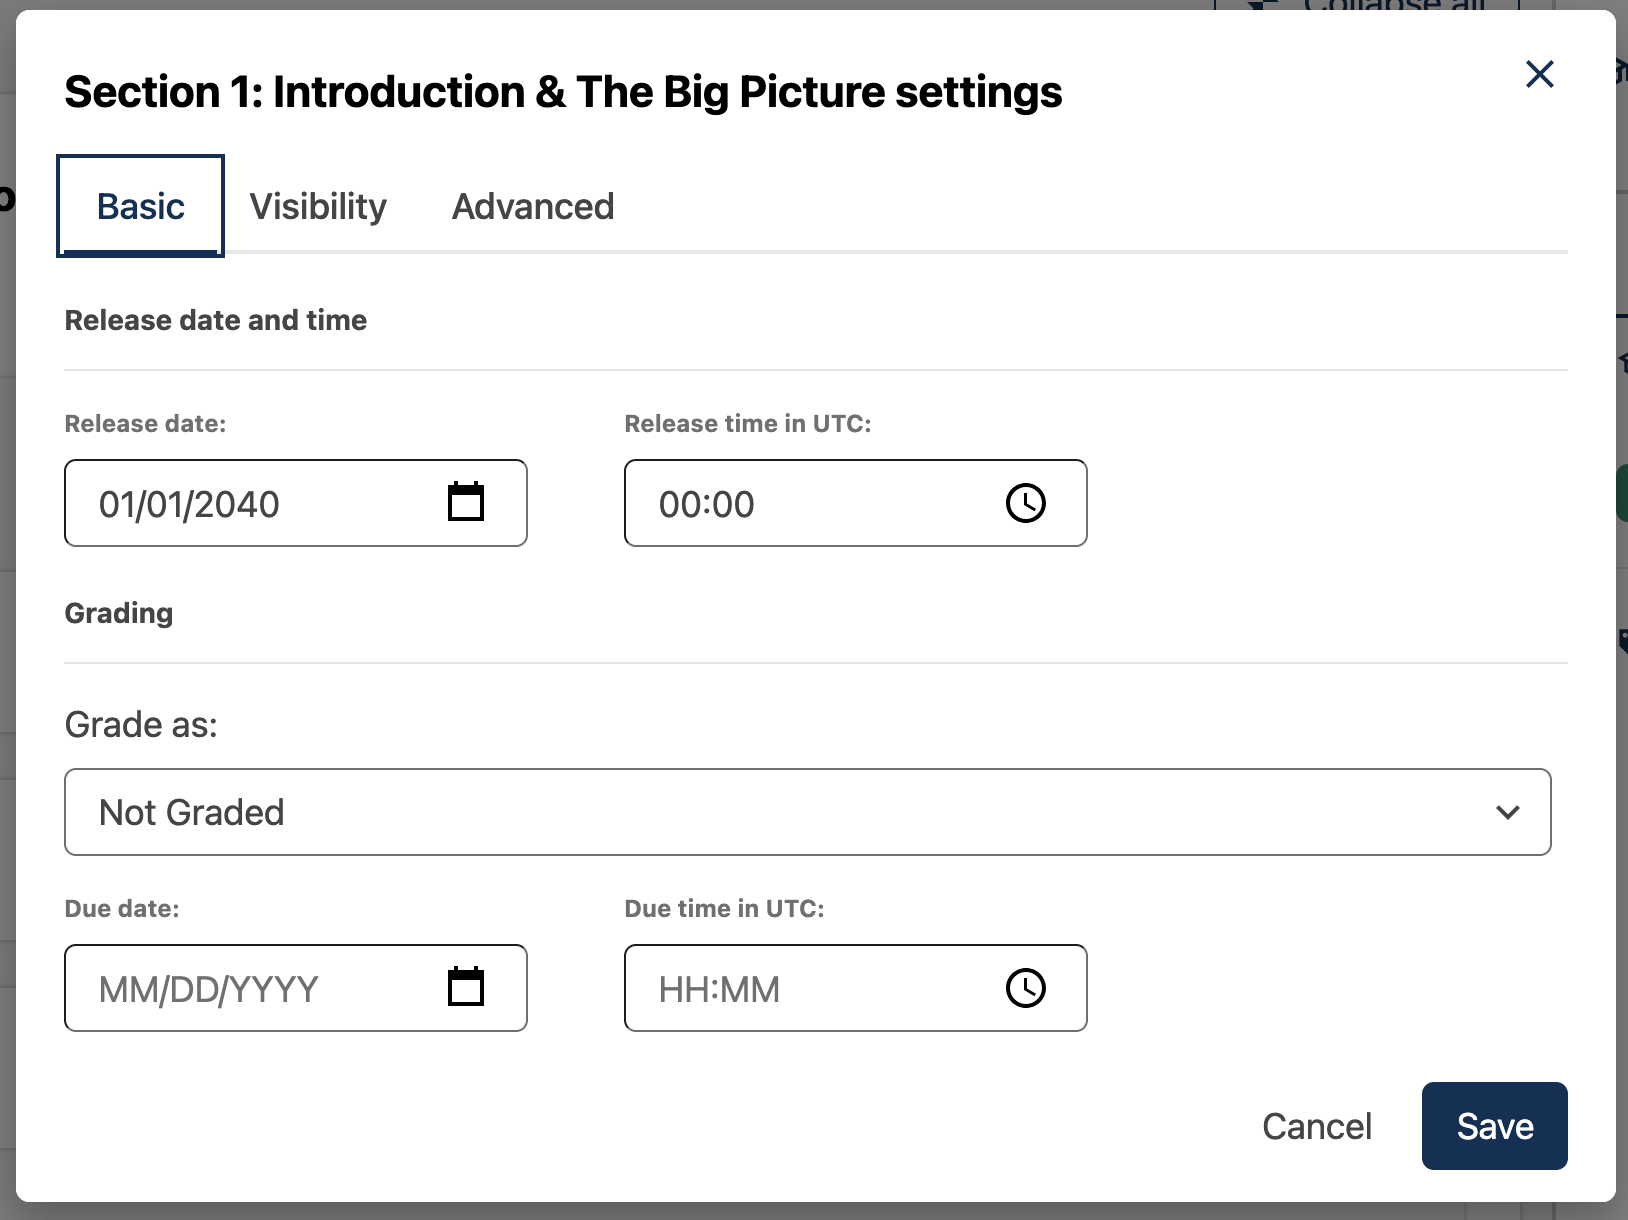
\includegraphics[width=\textwidth,height=0.6\textheight,keepaspectratio]{screenshots/visibility_settings.png}
\caption{Visibility \& Access Settings}
\label{fig:visibility-settings}
\end{figure}

\subsection{Components \& Activities}

\subsubsection{Dropdown Problem (UFR-OE-005-01)}
\begin{enumerate}
    \item Add a \textbf{Problem} component.
    \item Select \textbf{Dropdown} from the problem type.
    \item Enter the question text and options.
    \item Specify the correct answer.
    \item Save and publish.
\end{enumerate}

\subsubsection{Multi-Select Problem (UFR-OE-005-02)}
\begin{enumerate}
    \item Add a \textbf{Problem} component.
    \item Select \textbf{Multi-Select} (Checkbox) from the problem type.
    \item Enter the question text and multiple options.
    \item Mark the correct options.
    \item Save and publish.
\end{enumerate}

\subsubsection{Open Response Assessments (ORA) – UFR-OE-005-03}
\begin{enumerate}
    \item Add an \textbf{Advanced} component.
    \item Select \textbf{Open Response Assessment}.
    \item Define the \textbf{Prompt}: Describe the assignment question.
    \item Create the \textbf{Rubric}: Add criteria and scoring levels.
    \item Configure the assessment steps:
    \begin{itemize}
        \item \textbf{Self-Assessment}: Learners evaluate their own work.
        \item \textbf{Peer Assessment}: Learners review peers' submissions.
        \item \textbf{Staff Assessment}: Instructor provides final grade.
    \end{itemize}
    \item Set deadlines for each step.
    \item Save and publish.
\end{enumerate}

\begin{figure}[H]
\centering
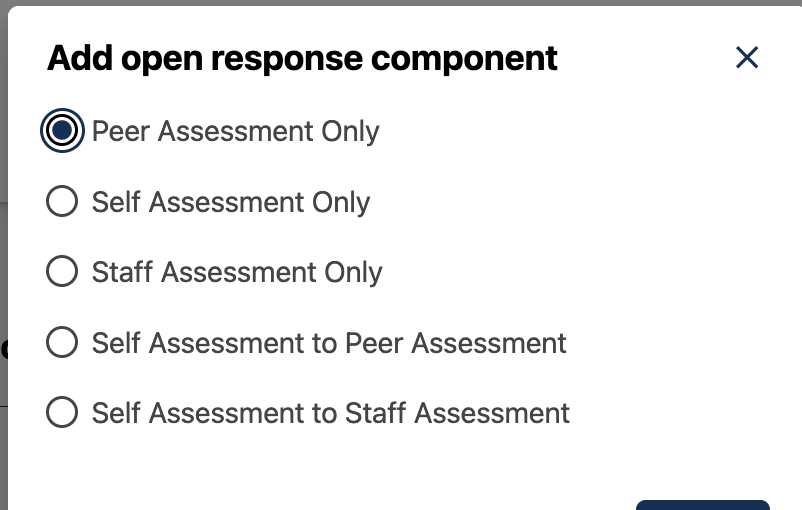
\includegraphics[width=\textwidth,height=0.6\textheight,keepaspectratio]{screenshots/ora_settings.png}
\caption{Open Response Assessment Settings}
\label{fig:ora-settings}
\end{figure}

\subsubsection{Single Select Problem (UFR-OE-005-04)}
\begin{enumerate}
    \item Add a \textbf{Problem} component.
    \item Select \textbf{Single Select} (Radio Button) from the problem type.
    \item Enter the question and options.
    \item Mark the correct answer.
    \item Save.
\end{enumerate}

\subsubsection{Text Input Problem (UFR-OE-005-05)}
\begin{enumerate}
    \item Add a \textbf{Problem} component.
    \item Select \textbf{Text Input} from the problem type.
    \item Enter the question.
    \item Specify the expected answer(s).
    \item Optionally add a hint or explanation.
    \item Save.
\end{enumerate}

\subsection{Data \& Analytics}

\subsubsection{View Course Enrollments (UFR-OE-006-01)}
\begin{enumerate}
    \item Navigate to the course \textbf{Instructor Dashboard}.
    \item Click \textbf{Data Downloads}.
    \item Select \textbf{Enrollment Data} to download a CSV report.
    \item View active enrollments, enrollment trends, and demographics.
\end{enumerate}

\begin{figure}[H]
\centering
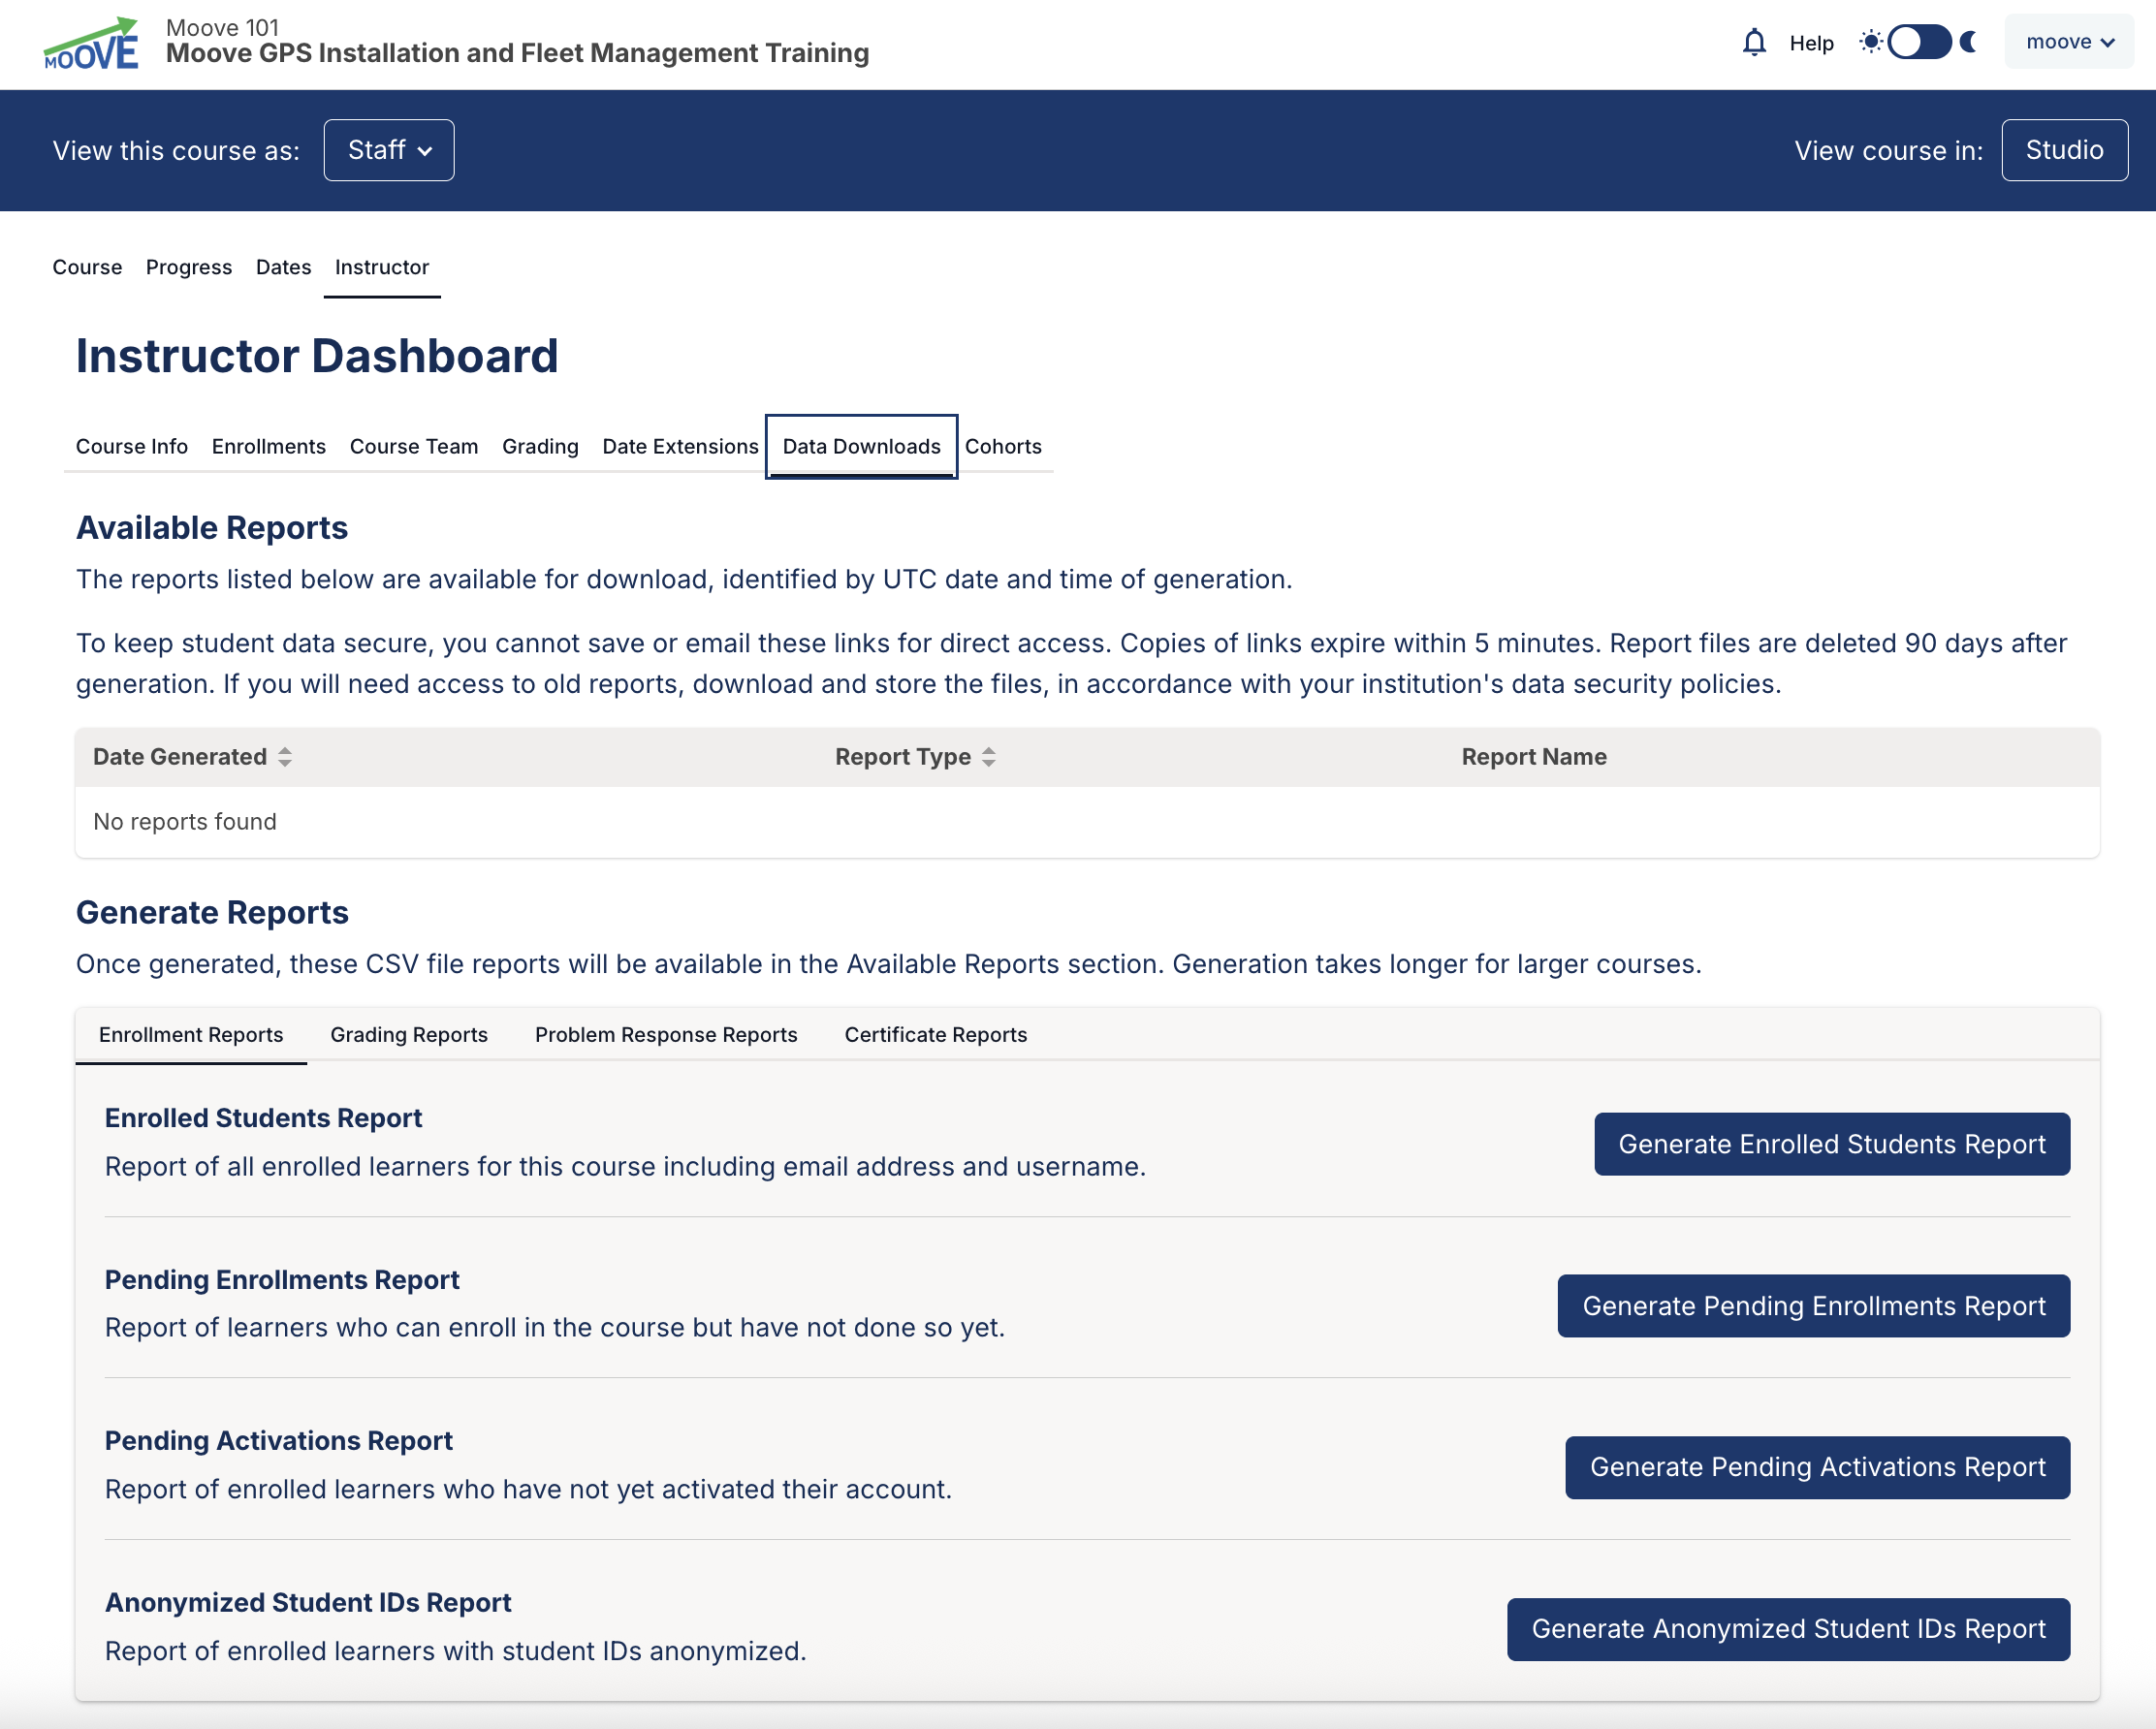
\includegraphics[width=\textwidth,height=0.6\textheight,keepaspectratio]{screenshots/enrollment_data.png}
\caption{Enrollment Data Report}
\label{fig:enrollment-data}
\end{figure}

\subsubsection{View Learner Data (UFR-OE-006-02)}
\begin{enumerate}
    \item Navigate to the course \textbf{Instructor Dashboard}.
    \item Click \textbf{Student Admin}.
    \item Search for a learner by email or username.
    \item View their activity history, progress, and grades.
\end{enumerate}

\subsubsection{View Learner Grades (UFR-OE-006-03)}
\begin{enumerate}
    \item Navigate to the course \textbf{Instructor Dashboard}.
    \item Click \textbf{Gradebook}.
    \item View all learners and their grades per assignment.
    \item To adjust a grade: click the grade cell, enter the new value, and save.
    \item Click \textbf{Export CSV} to download the gradebook.
\end{enumerate}

\begin{figure}[H]
\centering
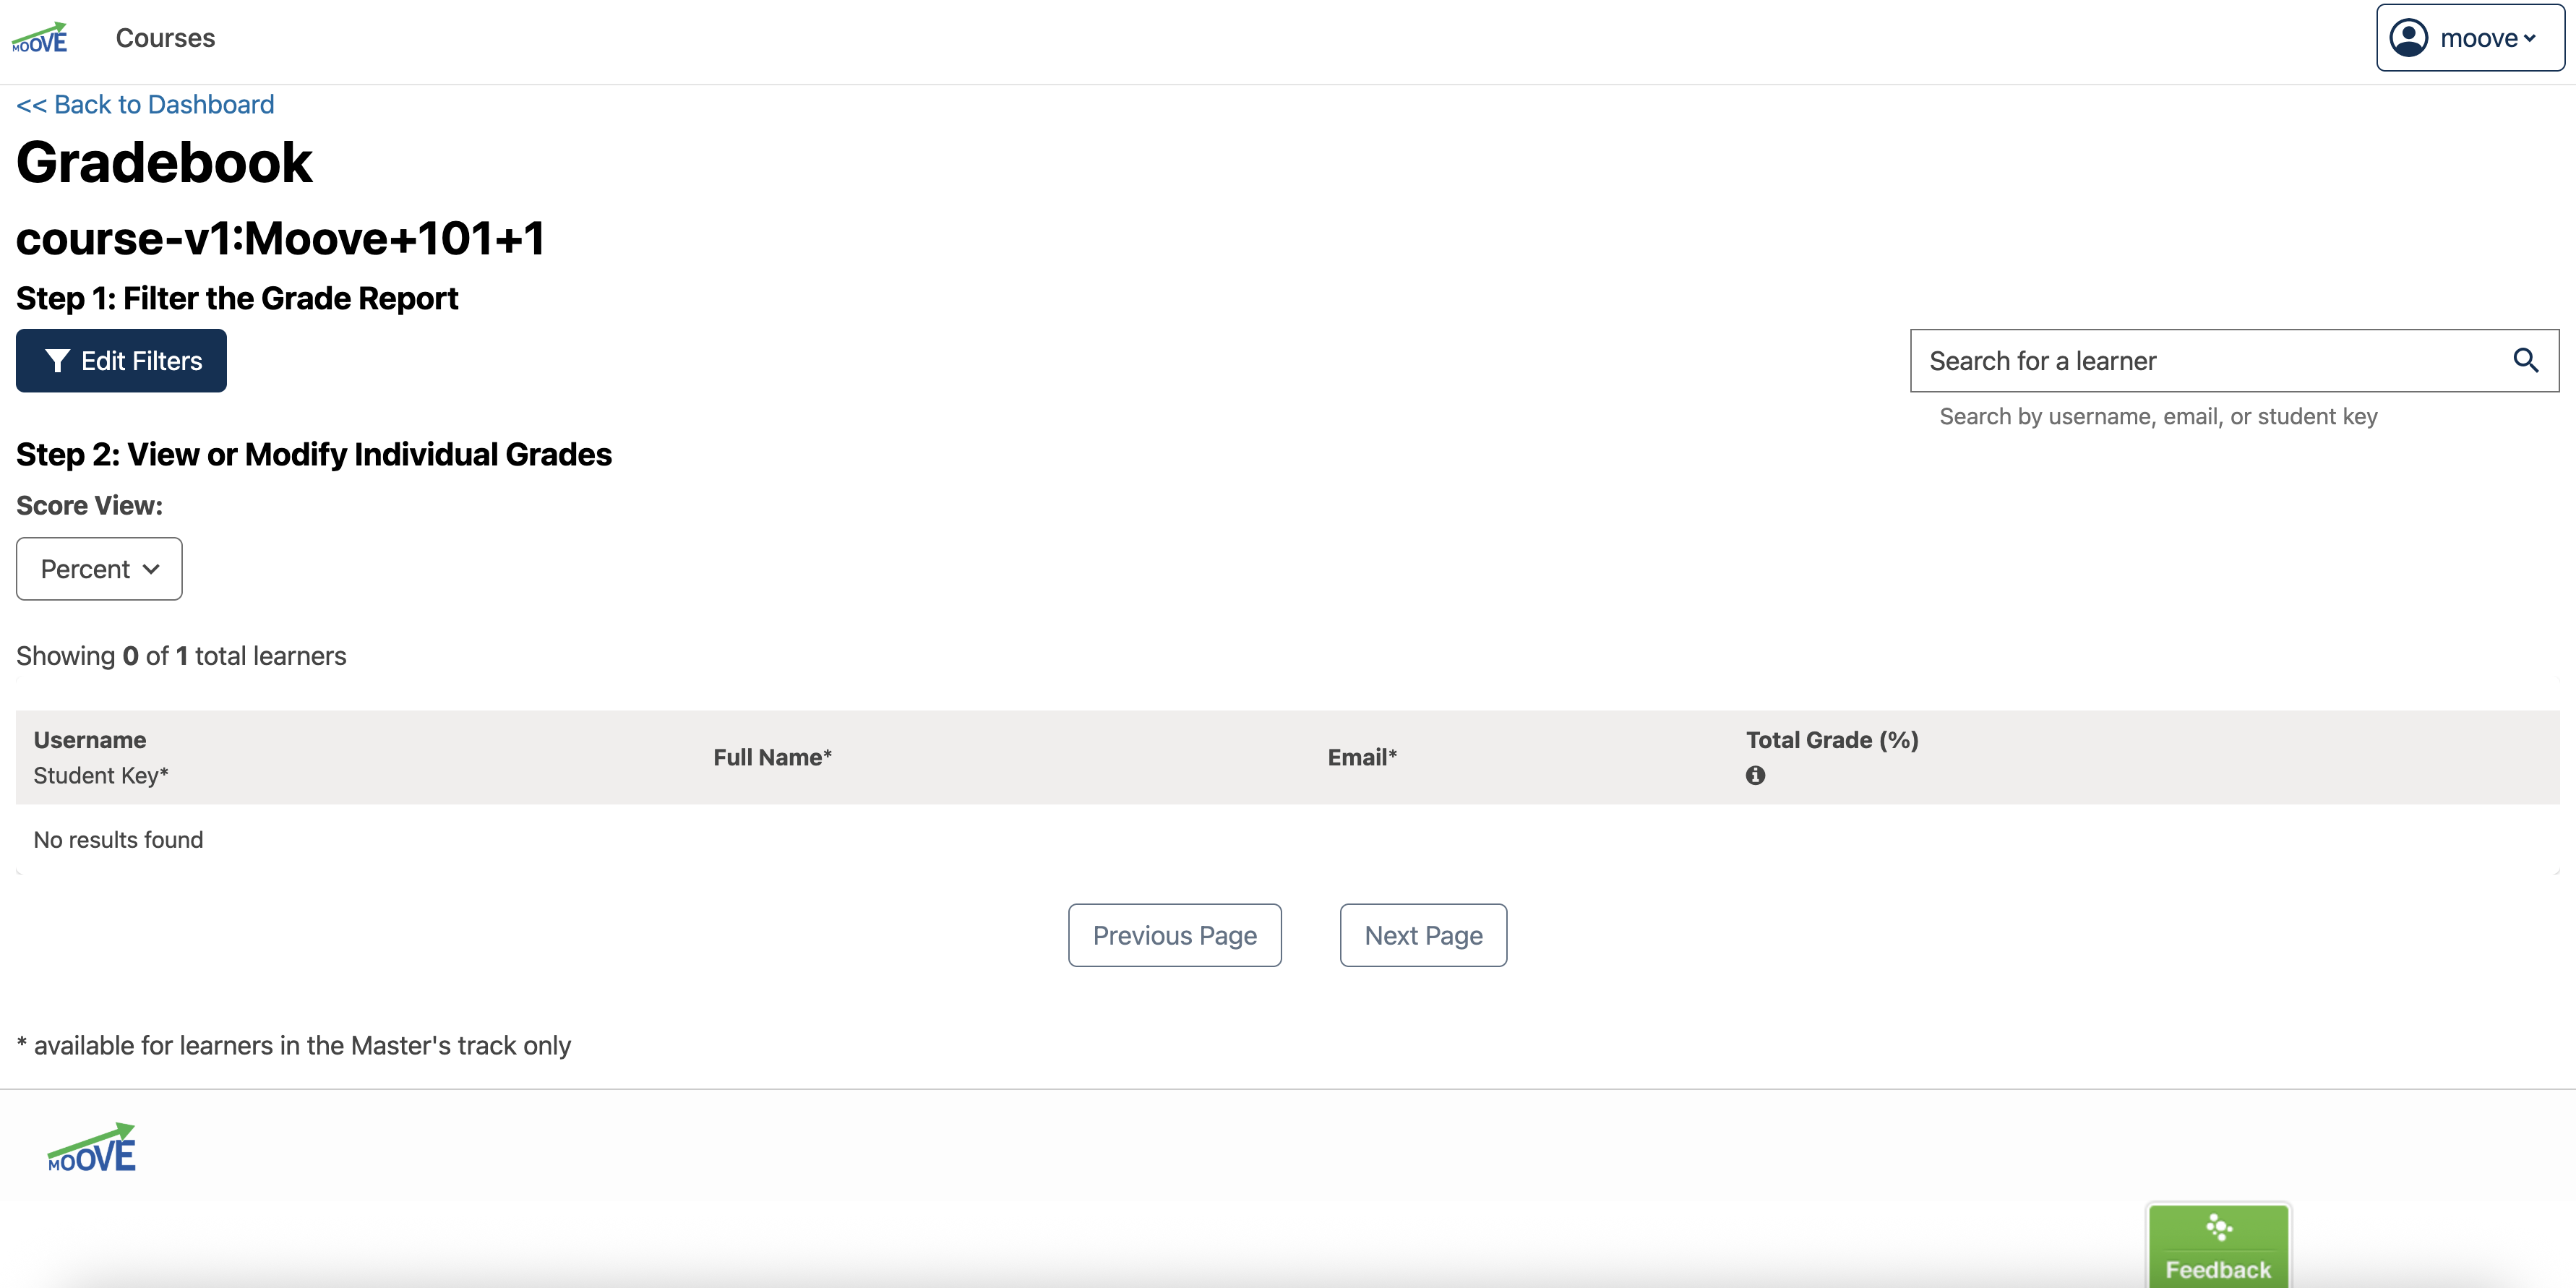
\includegraphics[width=\textwidth,height=0.6\textheight,keepaspectratio]{screenshots/gradebook.png}
\caption{Gradebook View}
\label{fig:gradebook}
\end{figure}

\subsubsection{View Answer Data (UFR-OE-006-04)}
\begin{enumerate}
    \item Navigate to the course \textbf{Instructor Dashboard}.
    \item Click \textbf{Data Downloads}.
    \item Select \textbf{Answer Distribution} to see how learners answered each problem.
    \item This helps identify difficult questions and improve the course.
\end{enumerate}

\subsubsection{View Certificate Data (UFR-OE-006-05)}
\begin{enumerate}
    \item Navigate to the course \textbf{Instructor Dashboard}.
    \item Click \textbf{Data Downloads}.
    \item Select \textbf{Certificate Data} to view issued certificates.
    \item Includes learner names, certificate URLs, and generation dates.
\end{enumerate}

\subsection{Accessibility}

\subsubsection{Open edX Accessibility Guidelines (UFR-OE-007-01)}
\begin{itemize}
    \item Follow the Open edX Accessibility Guidelines (WCAG 2.1 AA).
    \item Use descriptive alt text for all images.
    \item Ensure all videos have transcripts and captions.
    \item Test your course with screen readers.
\end{itemize}

\subsubsection{Design for Mobile Experience (UFR-OE-007-02)}
\begin{itemize}
    \item Test your course on mobile devices (phones and tablets).
    \item Ensure buttons and links are large enough to tap.
    \item Avoid complex interactions that don't work on touch screens.
\end{itemize}

\subsubsection{Accessibility Best Practices Checklist (UFR-OE-007-03)}
\begin{itemize}
    \item \textbf{Alt Text}: All images and figures have descriptive text.
    \item \textbf{Headings}: Use proper heading hierarchy (H1, H2, H3, etc.).
    \item \textbf{Color Contrast}: Ensure sufficient contrast ratios.
    \item \textbf{Keyboard Navigation}: All functionality works with keyboard only.
    \item \textbf{Descriptive Links}: Link text describes the destination.
\end{itemize}

\subsubsection{Manage Video Transcripts (UFR-OE-007-04)}
\begin{enumerate}
    \item Upload a video component.
    \item Click \textbf{Upload Transcript}.
    \item Select an \texttt{.srt} or \texttt{.vtt} file.
    \item The transcript will appear as closed captions in the video player.
\end{enumerate}

\begin{figure}[H]
\centering
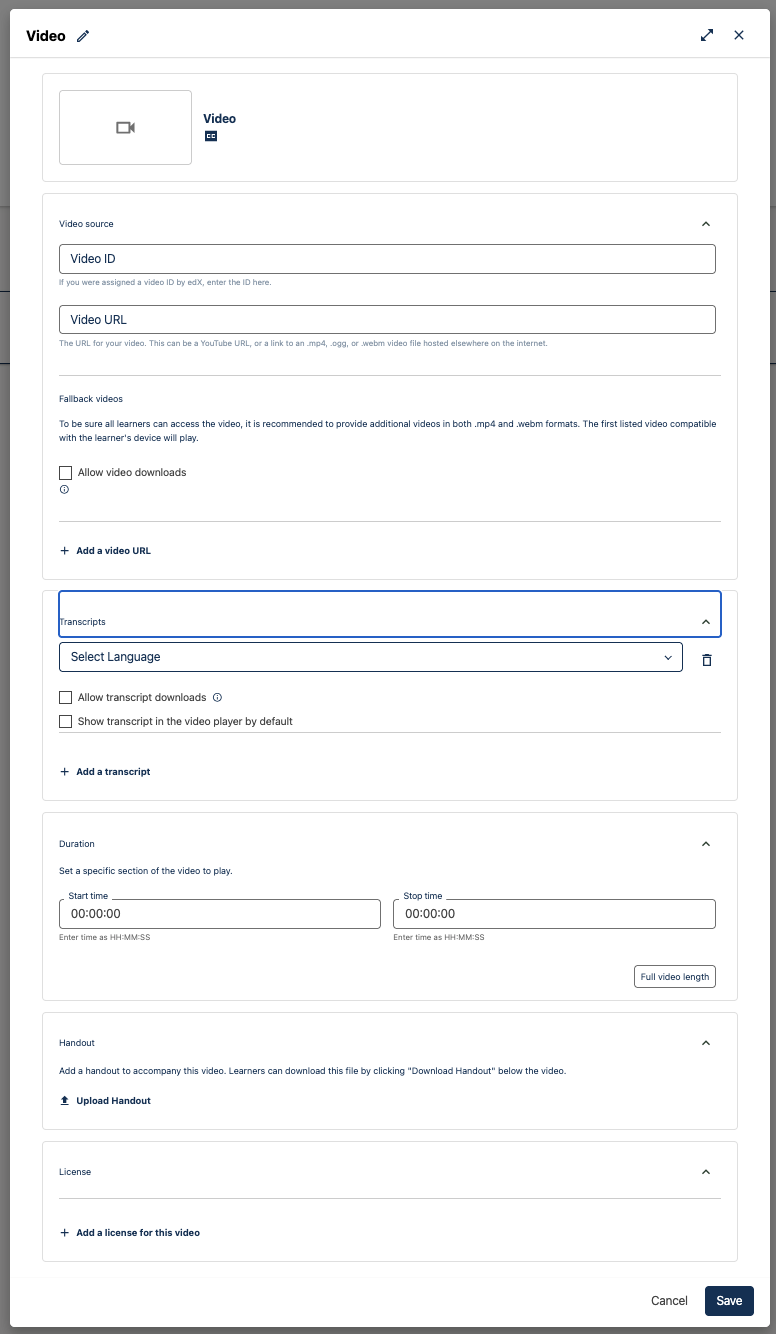
\includegraphics[width=\textwidth,height=0.6\textheight,keepaspectratio]{screenshots/transcript_upload.png}
\caption{Transcript Upload}
\label{fig:transcript-upload}
\end{figure}

\subsection{Import/Export / OLX}

\subsubsection{Open Learning XML (OLX) Support (UFR-OE-008-01)}
\begin{enumerate}
    \item To export a course: go to the course \textbf{Settings} page.
    \item Click \textbf{Export Course}.
    \item The system will generate a \texttt{.tar.gz} file containing OLX files.
    \item To import: click \textbf{Import Course}, select the file, and upload.
    \item The course structure and content will be recreated.
\end{enumerate}

\begin{figure}[H]
\centering
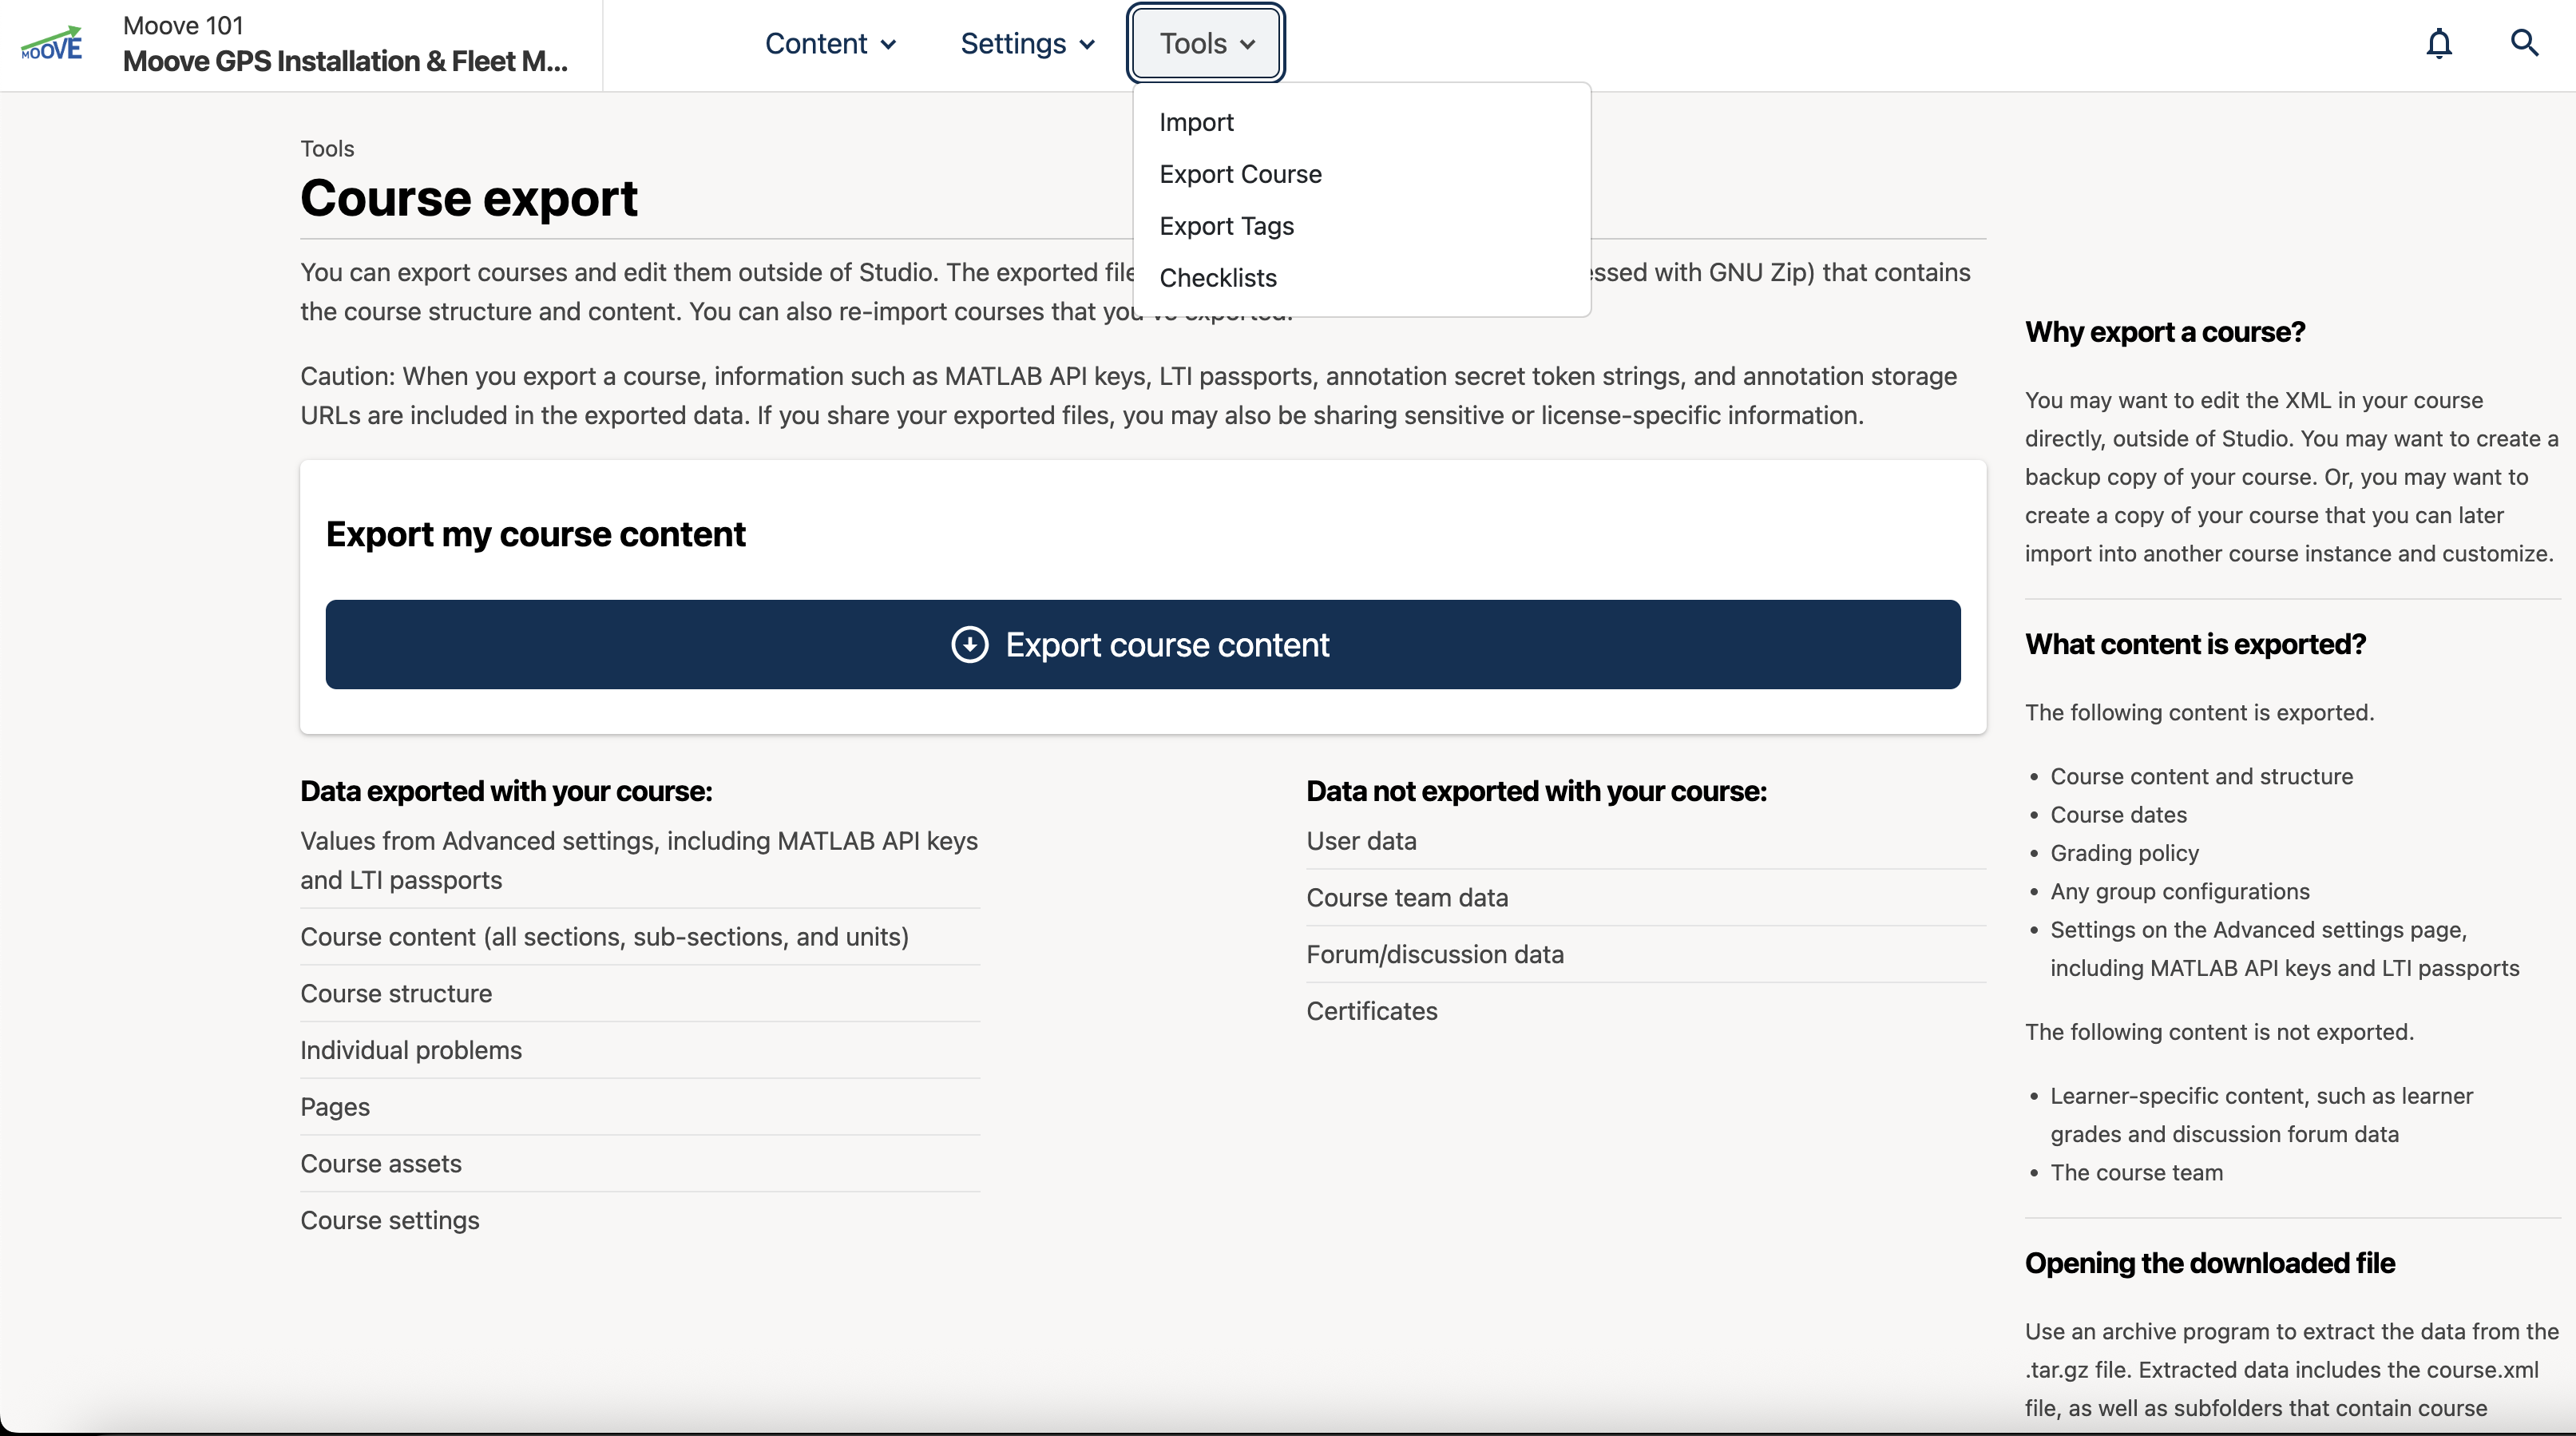
\includegraphics[width=\textwidth,height=0.6\textheight,keepaspectratio]{screenshots/export_course.png}
\caption{Course Export/Import}
\label{fig:export-course}
\end{figure}

\subsubsection{Getting Started with OLX (UFR-OE-008-02)}
\begin{itemize}
    \item OLX (Open Learning XML) is the standard format for Open edX course content.
    \item It allows you to build courses programmatically or migrate from other systems.
    \item Documentation is available at the Open edX Developer Documentation.
    \item Use the \texttt{olx} command-line tool for validation.
\end{itemize}

\section{Learner Features}
This section covers all features available to learners (students).

\subsection{Dashboard \& Profile}

\subsubsection{Exploring Your Dashboard and Profile (UFR-OE-101-01)}
\begin{enumerate}
    \item Log in to the platform at \texttt{educationvirtual.net}.
    \item Your dashboard shows: enrolled courses, recent activity, announcements.
    \item Click your avatar in the top-right corner to access your profile.
\end{enumerate}

\begin{figure}[H]
\centering
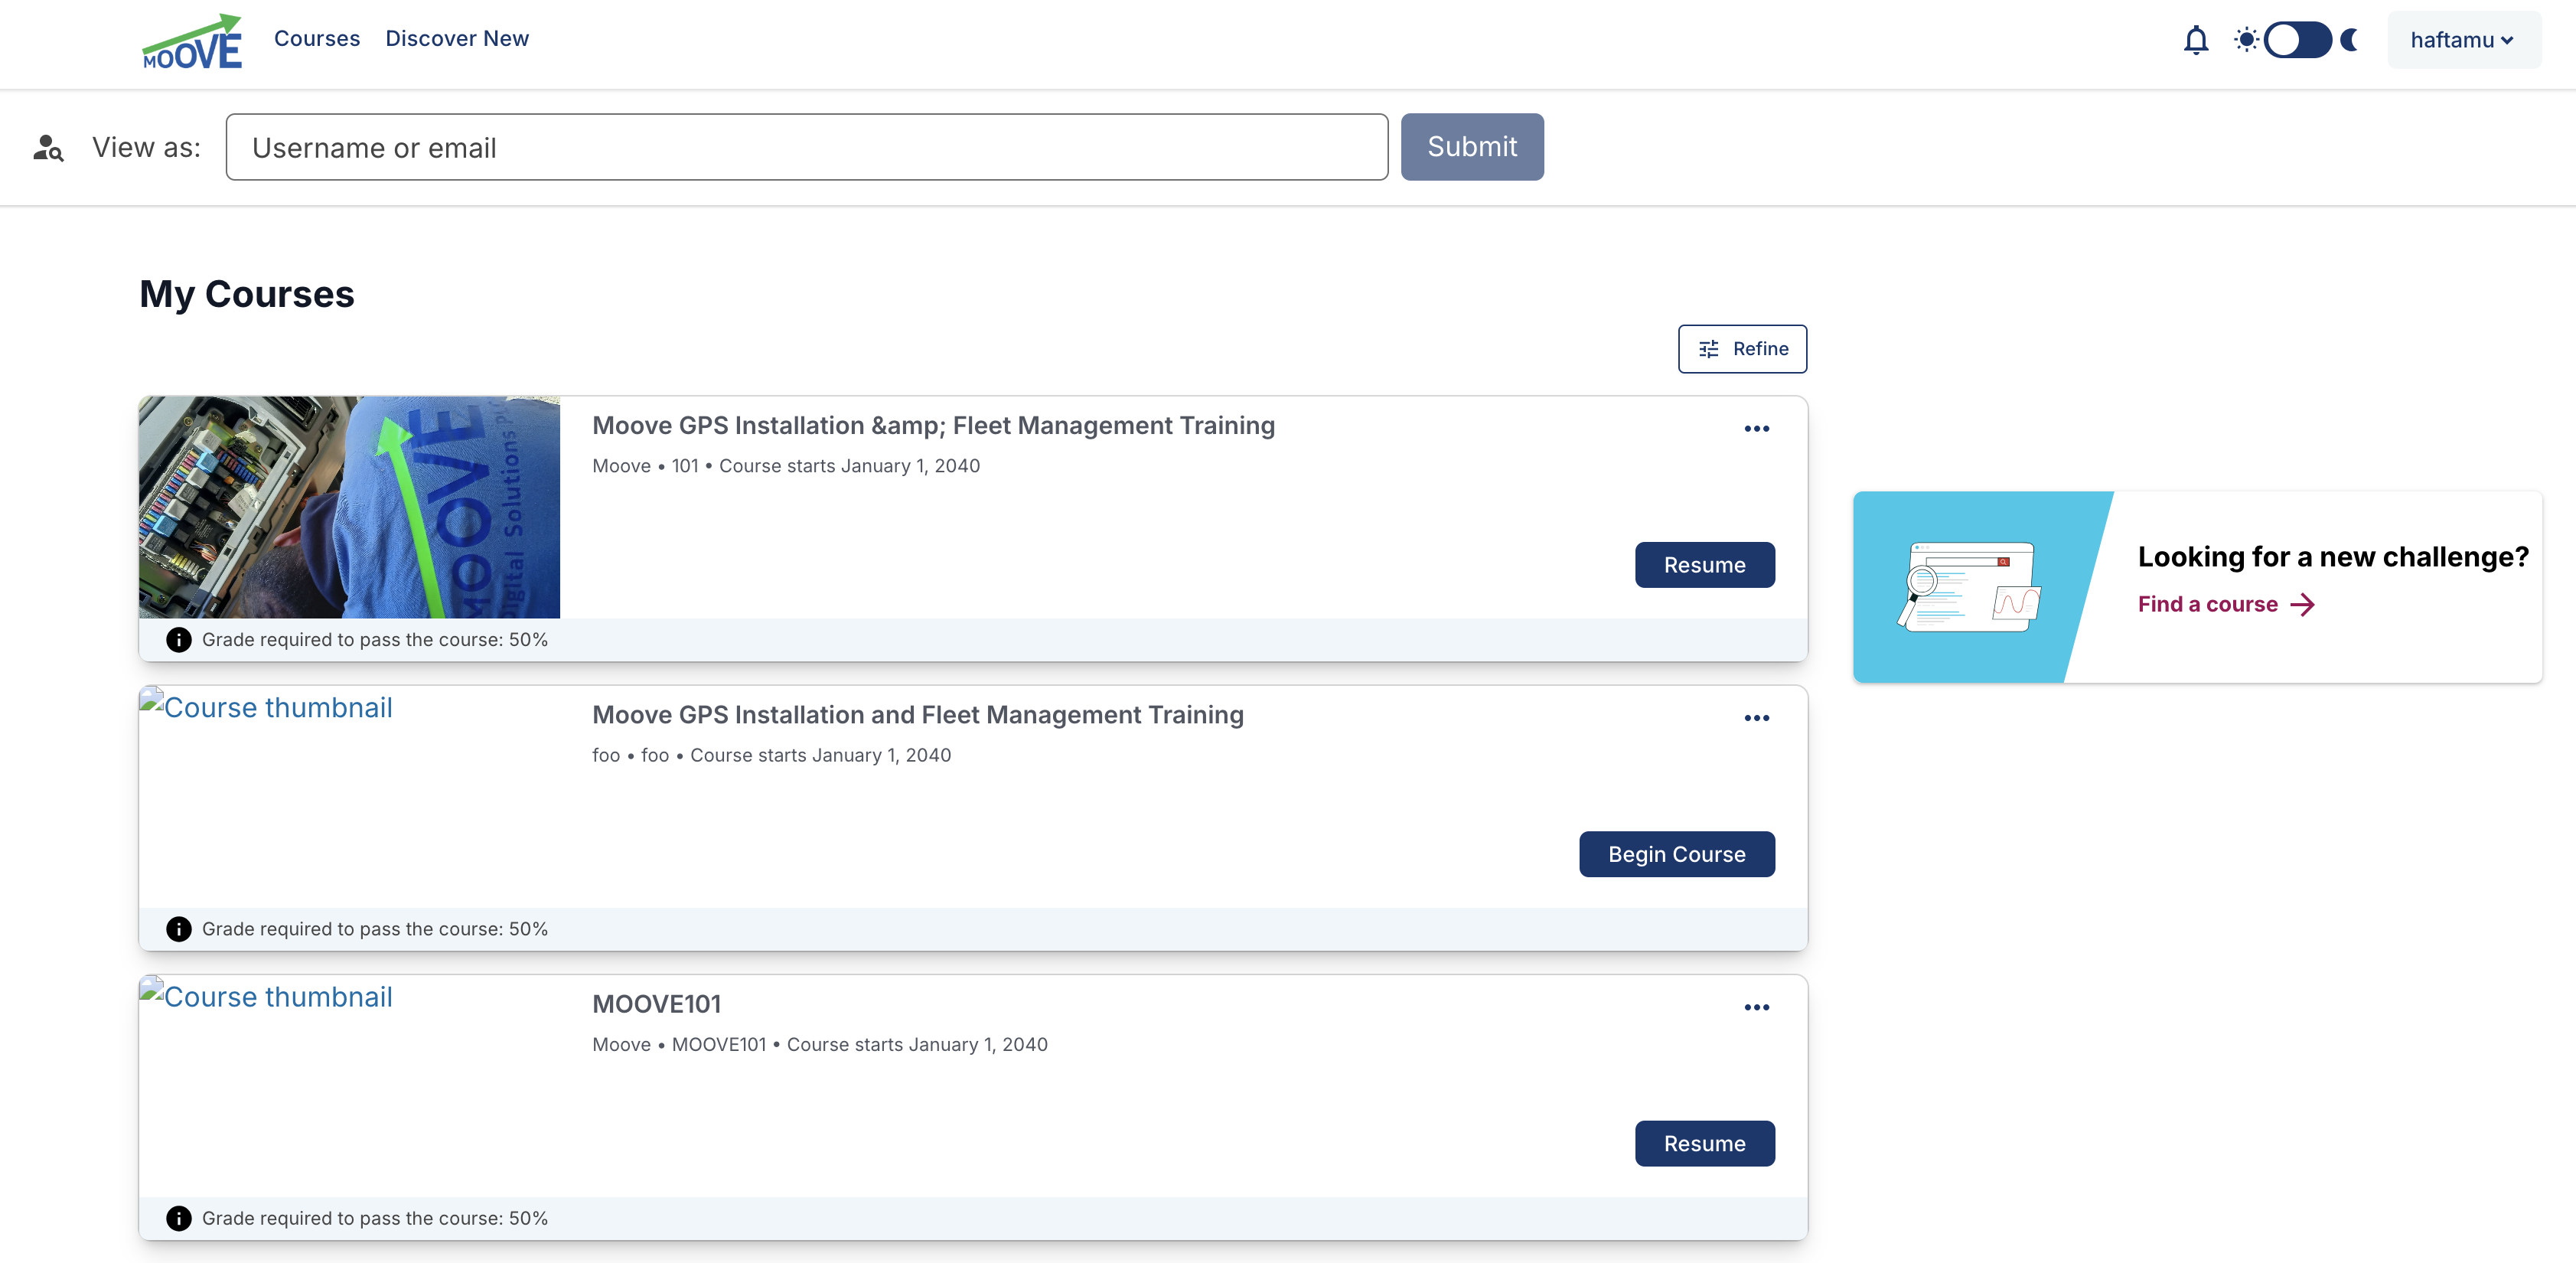
\includegraphics[width=\textwidth,height=0.6\textheight,keepaspectratio]{screenshots/dashboard.png}
\caption{Learner Dashboard}
\label{fig:dashboard}
\end{figure}

\subsubsection{Access Your Courses from the Dashboard (UFR-OE-101-02)}
\begin{enumerate}
    \item From your dashboard, click the course card of the course you want to access.
    \item You will be taken to the course home page.
\end{enumerate}

\subsubsection{Share Your Courses on Social Media (UFR-OE-101-03)}
\begin{enumerate}
    \item Go to the course page.
    \item Click the \textbf{Share} icon.
    \item Select the social media platform (Facebook, Twitter, LinkedIn).
    \item The course link will be shared.
\end{enumerate}

\subsubsection{Update Your Profile Image (UFR-OE-101-04)}
\begin{enumerate}
    \item Go to your profile page.
    \item Click the camera icon on your profile picture.
    \item Select an image file from your device.
    \item The image will be uploaded and resized.
\end{enumerate}

\subsubsection{Update Your Profile Details (UFR-OE-101-05)}
\begin{enumerate}
    \item Go to your profile page.
    \item Click \textbf{Edit Profile}.
    \item Update your name, email, location, bio, language preferences.
    \item Click \textbf{Save}.
\end{enumerate}

\begin{figure}[H]
\centering
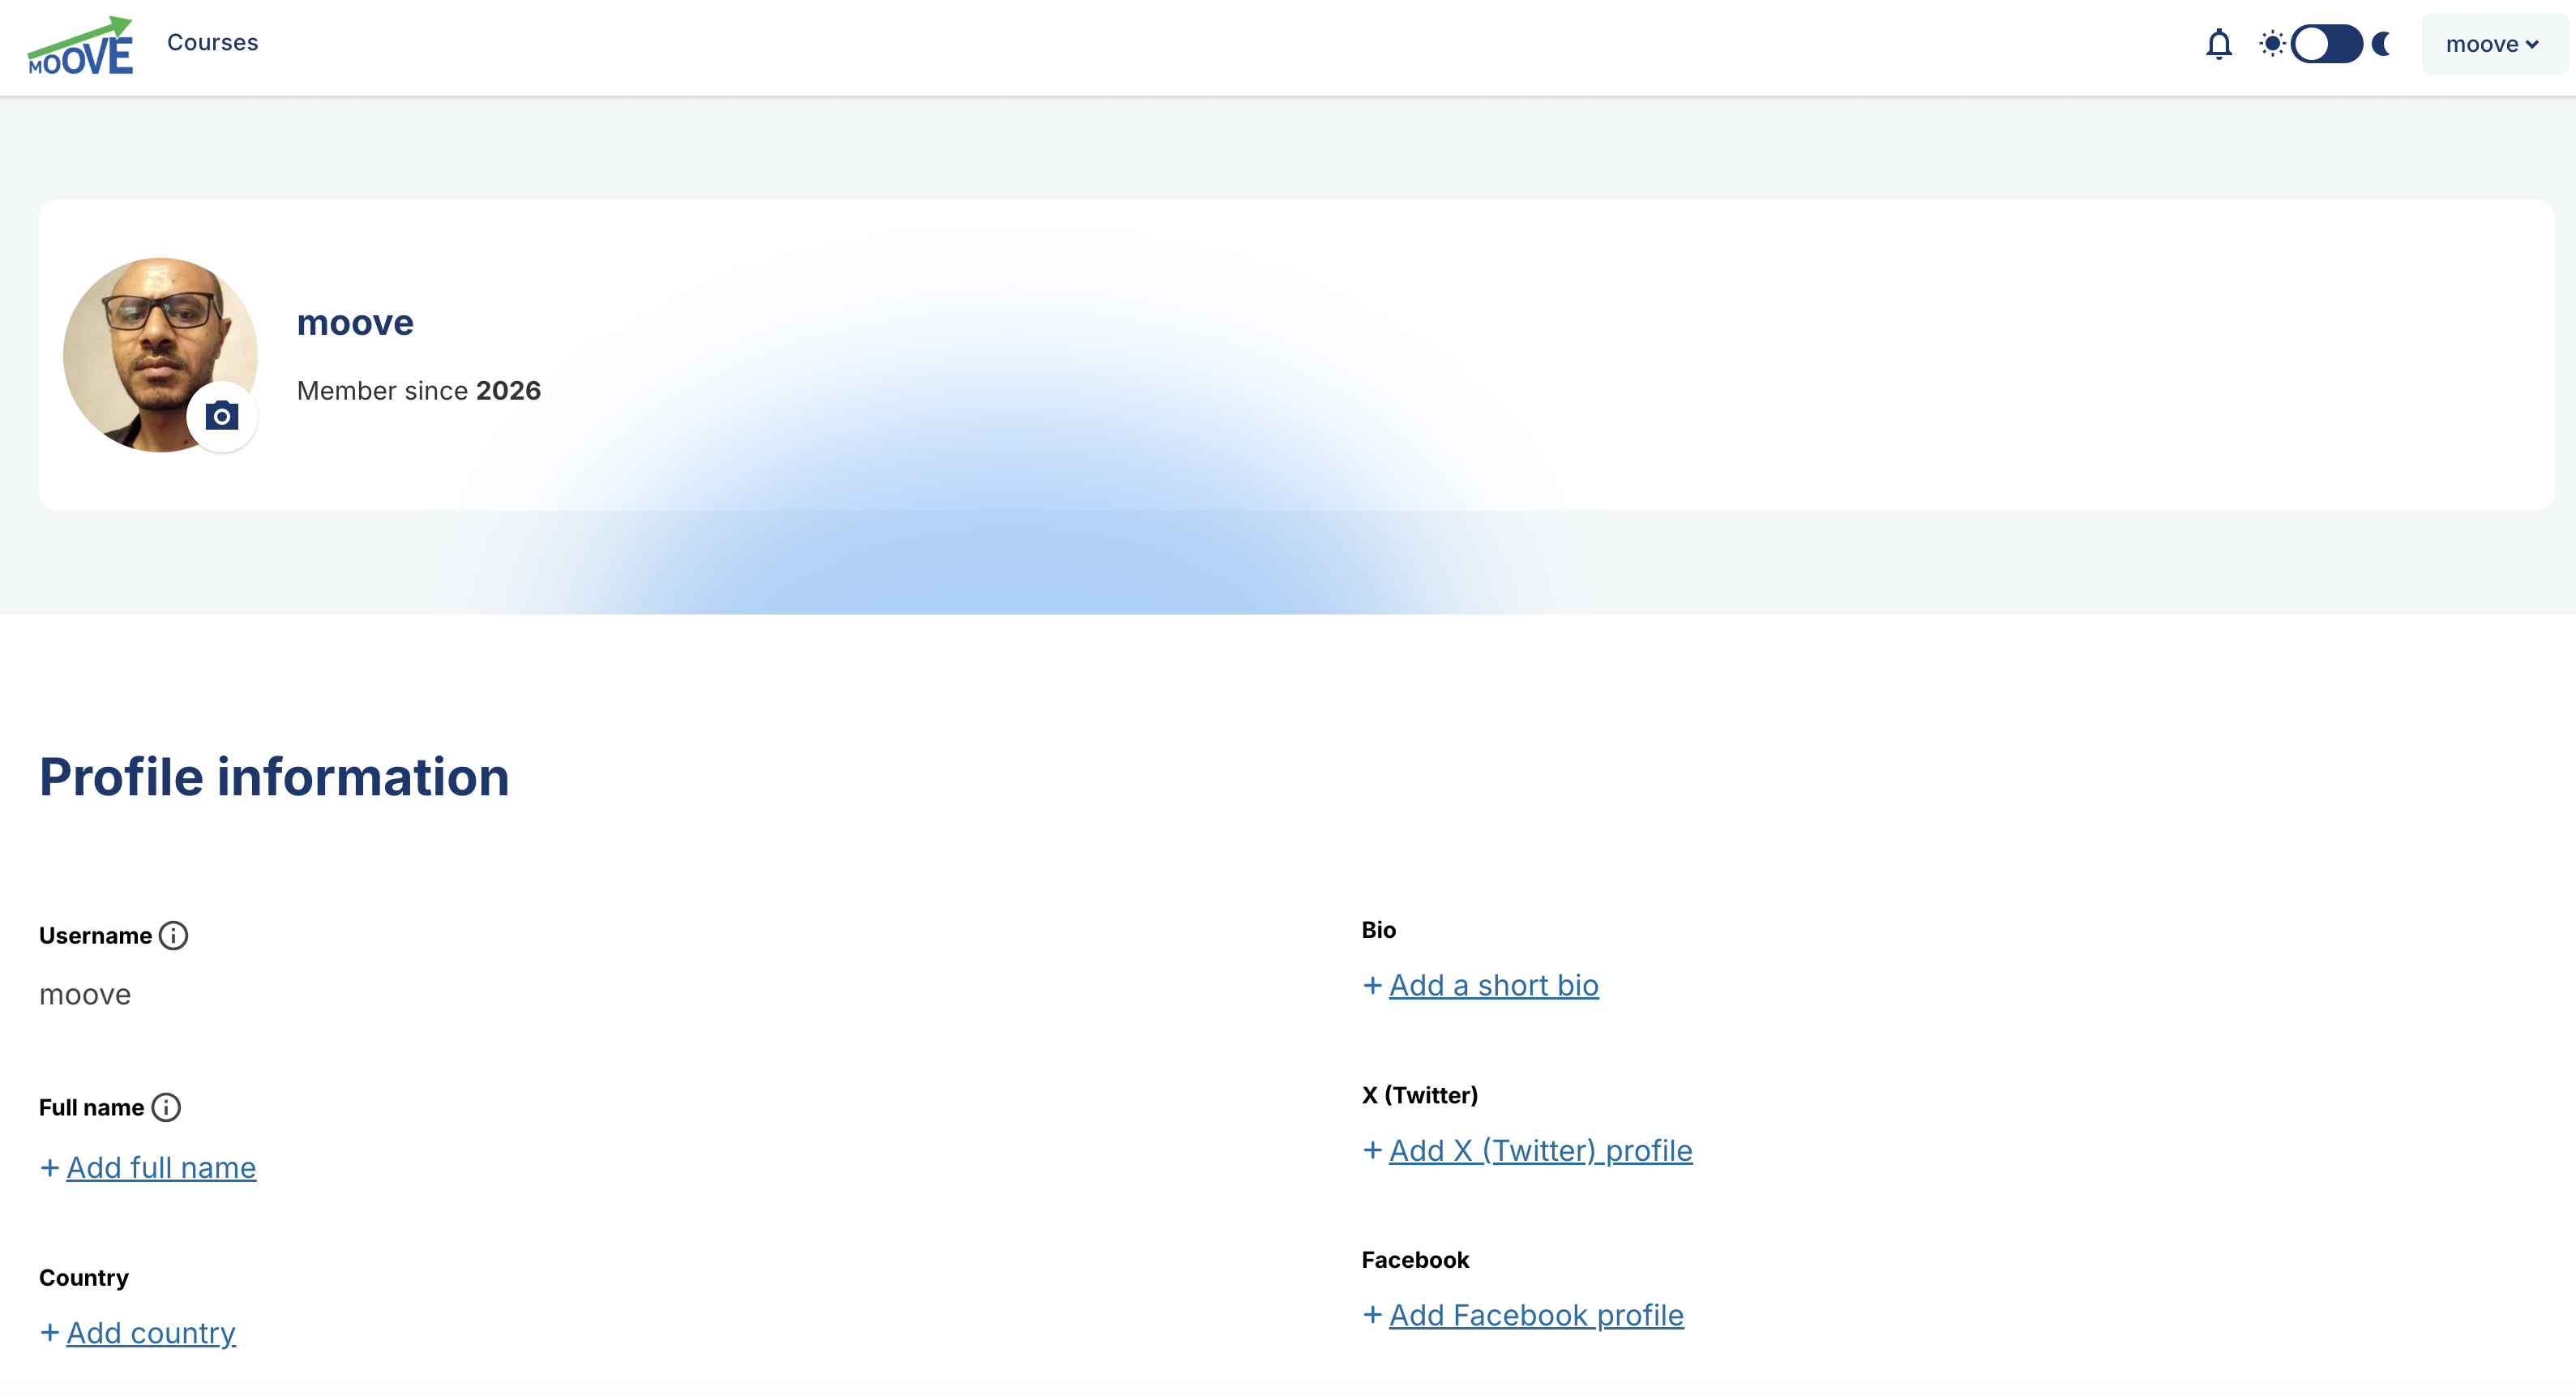
\includegraphics[width=\textwidth,height=0.6\textheight,keepaspectratio]{screenshots/profile_edit.png}
\caption{Profile Edit Form}
\label{fig:profile-edit}
\end{figure}

\subsubsection{Add Links to Your Personal Social Media Accounts (UFR-OE-101-06)}
\begin{enumerate}
    \item Go to your profile page.
    \item Click \textbf{Edit Profile}.
    \item Enter URLs for Twitter, LinkedIn, GitHub, etc.
    \item Click \textbf{Save}. Icons will appear on your profile.
\end{enumerate}

\subsubsection{Toggle Profile Information Visibility (UFR-OE-101-07)}
\begin{enumerate}
    \item Go to your profile page.
    \item Click \textbf{Edit Profile}.
    \item Toggle \textbf{Make Profile Public} to control visibility.
    \item Click \textbf{Save}.
\end{enumerate}

\subsubsection{View Another Learner’s Profile (UFR-OE-101-08)}
\begin{enumerate}
    \item Click on a learner's username in a discussion post or course roster.
    \item Their profile page will open (limited to public information).
\end{enumerate}

\subsubsection{Updating Course-Specific Settings (UFR-OE-101-09)}
\begin{enumerate}
    \item Enter a course.
    \item Click your avatar, then \textbf{Course Settings}.
    \item Adjust email notifications, language preference, etc.
    \item Click \textbf{Save}.
\end{enumerate}

\subsection{Course Navigation}

\subsubsection{View Course Sections from the Navigation Sidebar (UFR-OE-102-01)}
\begin{enumerate}
    \item In a course, look at the left sidebar.
    \item It displays all sections (weeks/modules) and subsections.
    \item Click any item to navigate directly to that content.
\end{enumerate}

\begin{figure}[H]
\centering
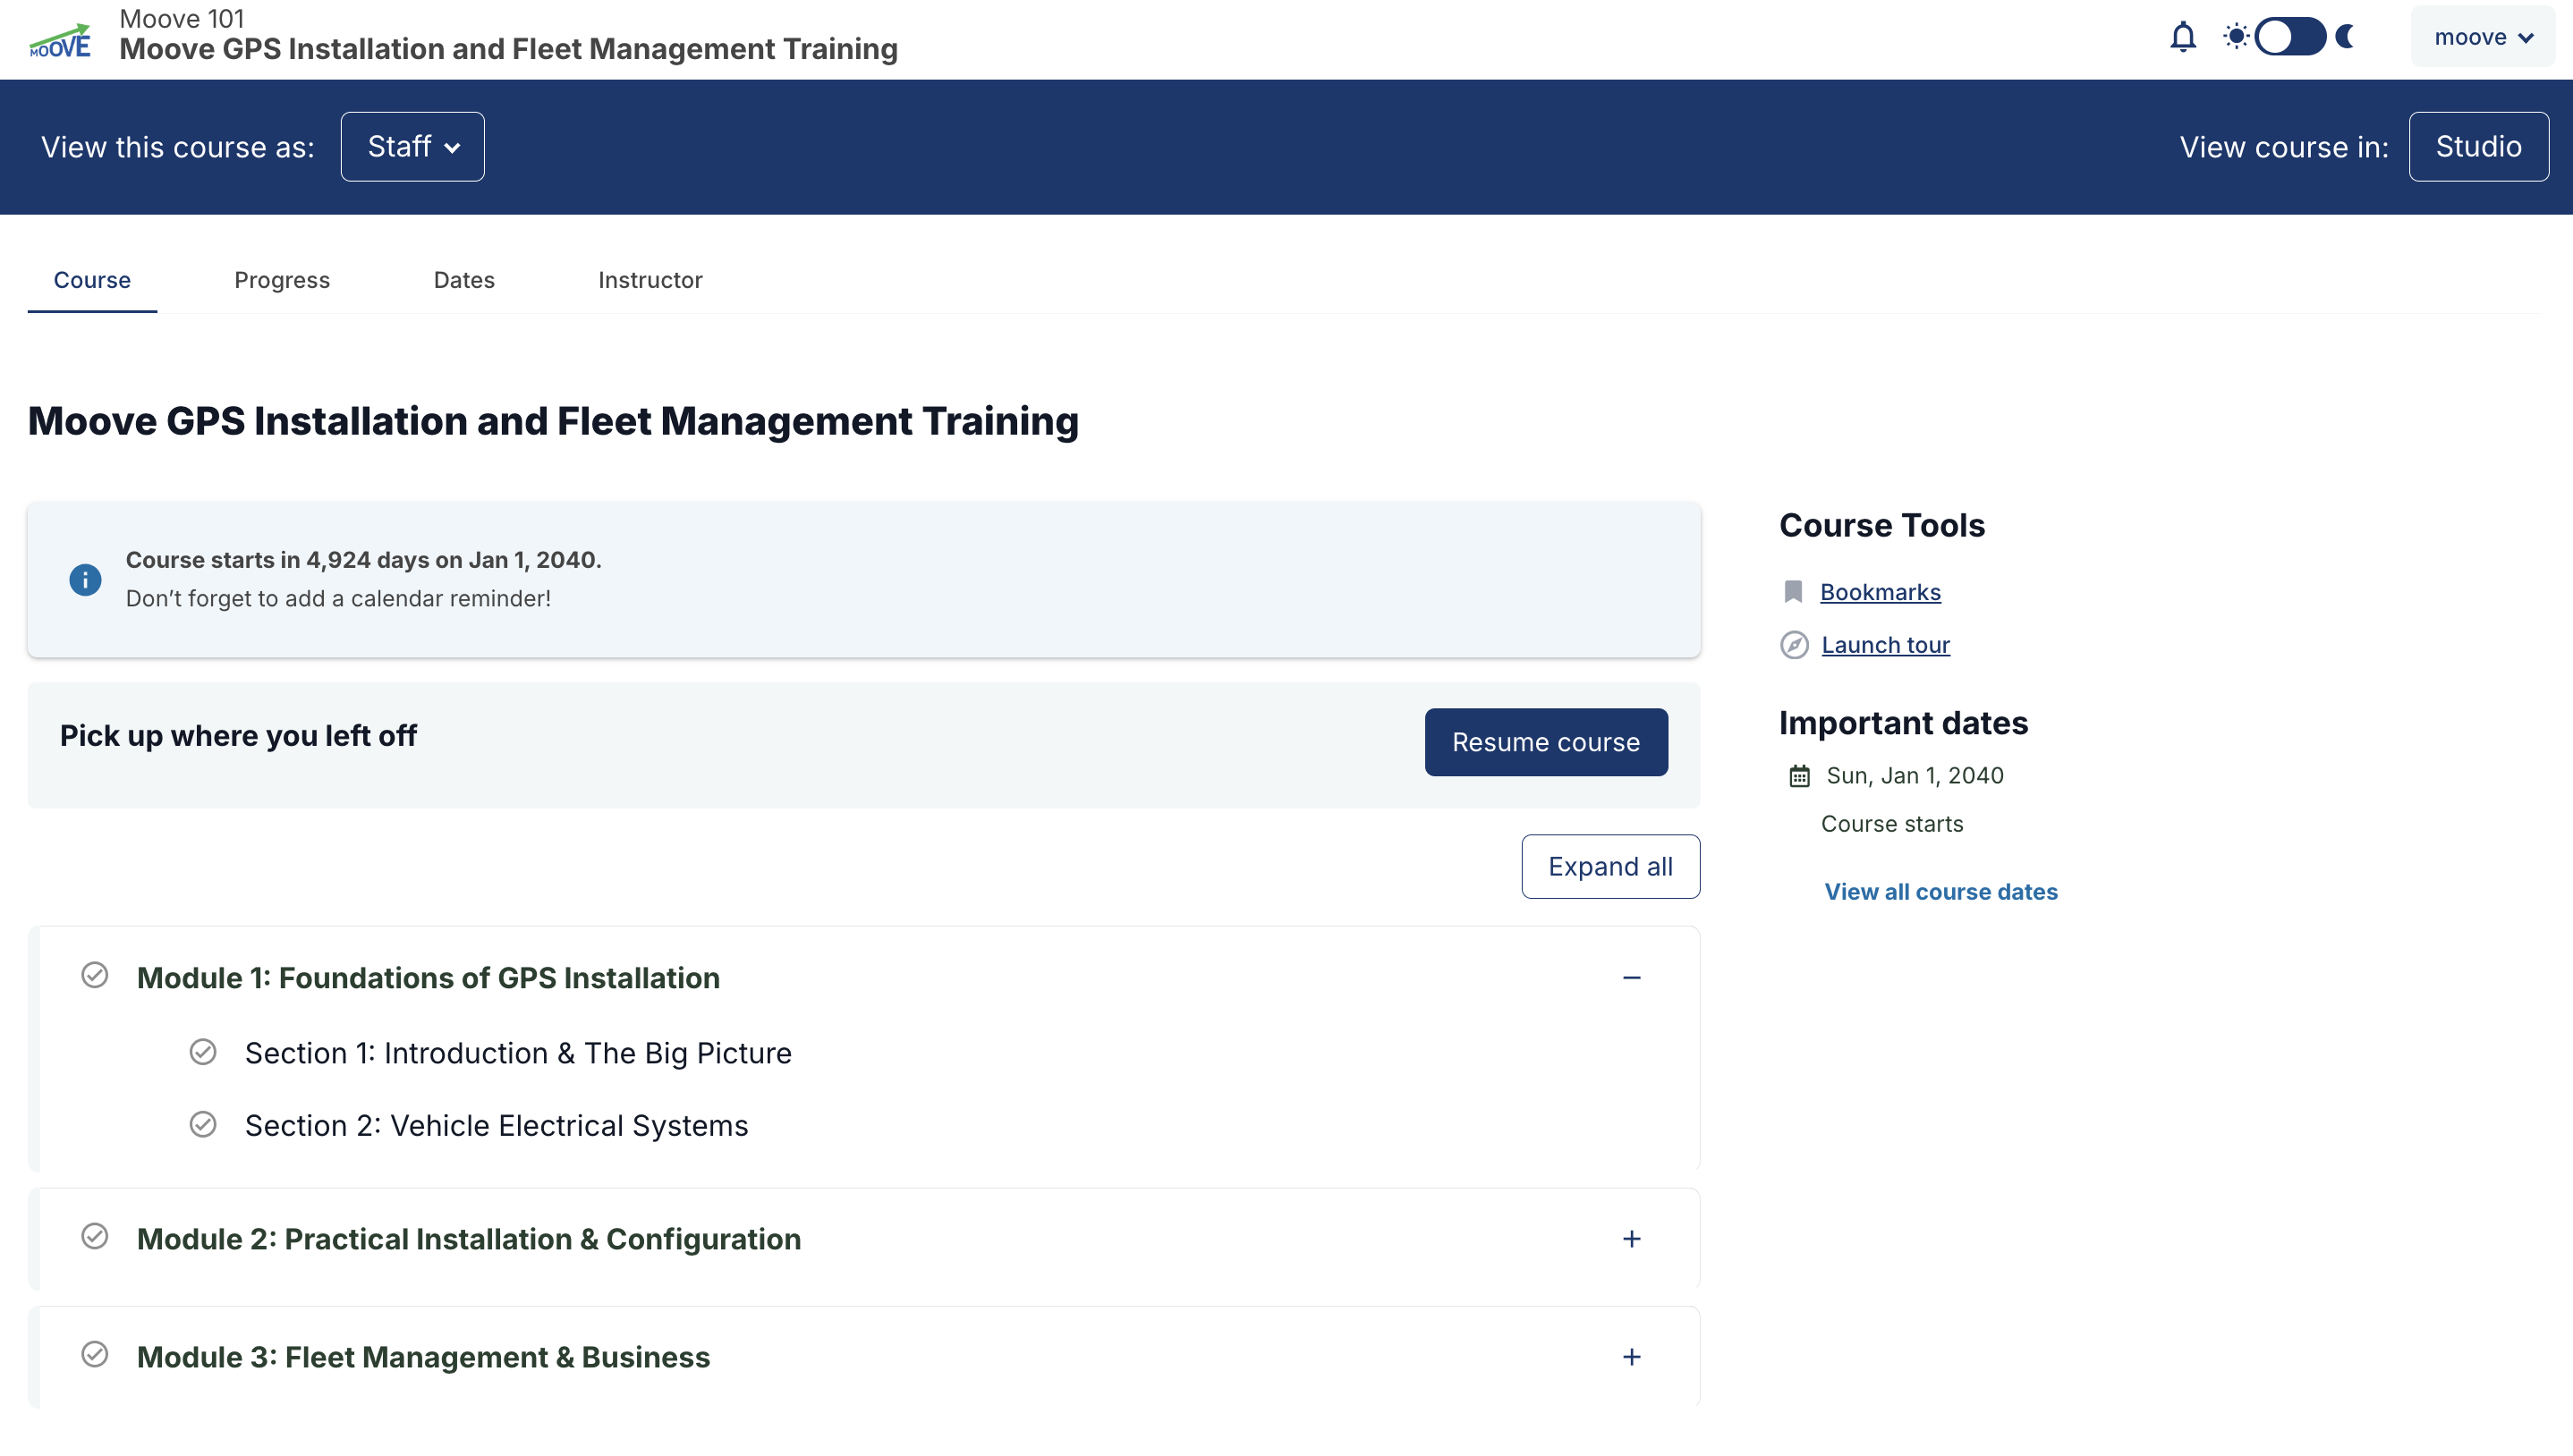
\includegraphics[width=\textwidth,height=0.6\textheight,keepaspectratio]{screenshots/sidebar_navigation.png}
\caption{Sidebar Navigation}
\label{fig:sidebar-navigation}
\end{figure}

\subsection{Enrollment}

\subsubsection{Enroll in a Course (UFR-OE-103-01)}
\begin{enumerate}
    \item Browse the course catalog or search for a course.
    \item Click on the course to open its info page.
    \item Click \textbf{Enroll Now}.
    \item Select enrollment mode (Audit/Verified).
    \item Click \textbf{Enroll}. You are now enrolled.
\end{enumerate}

\begin{figure}[H]
\centering
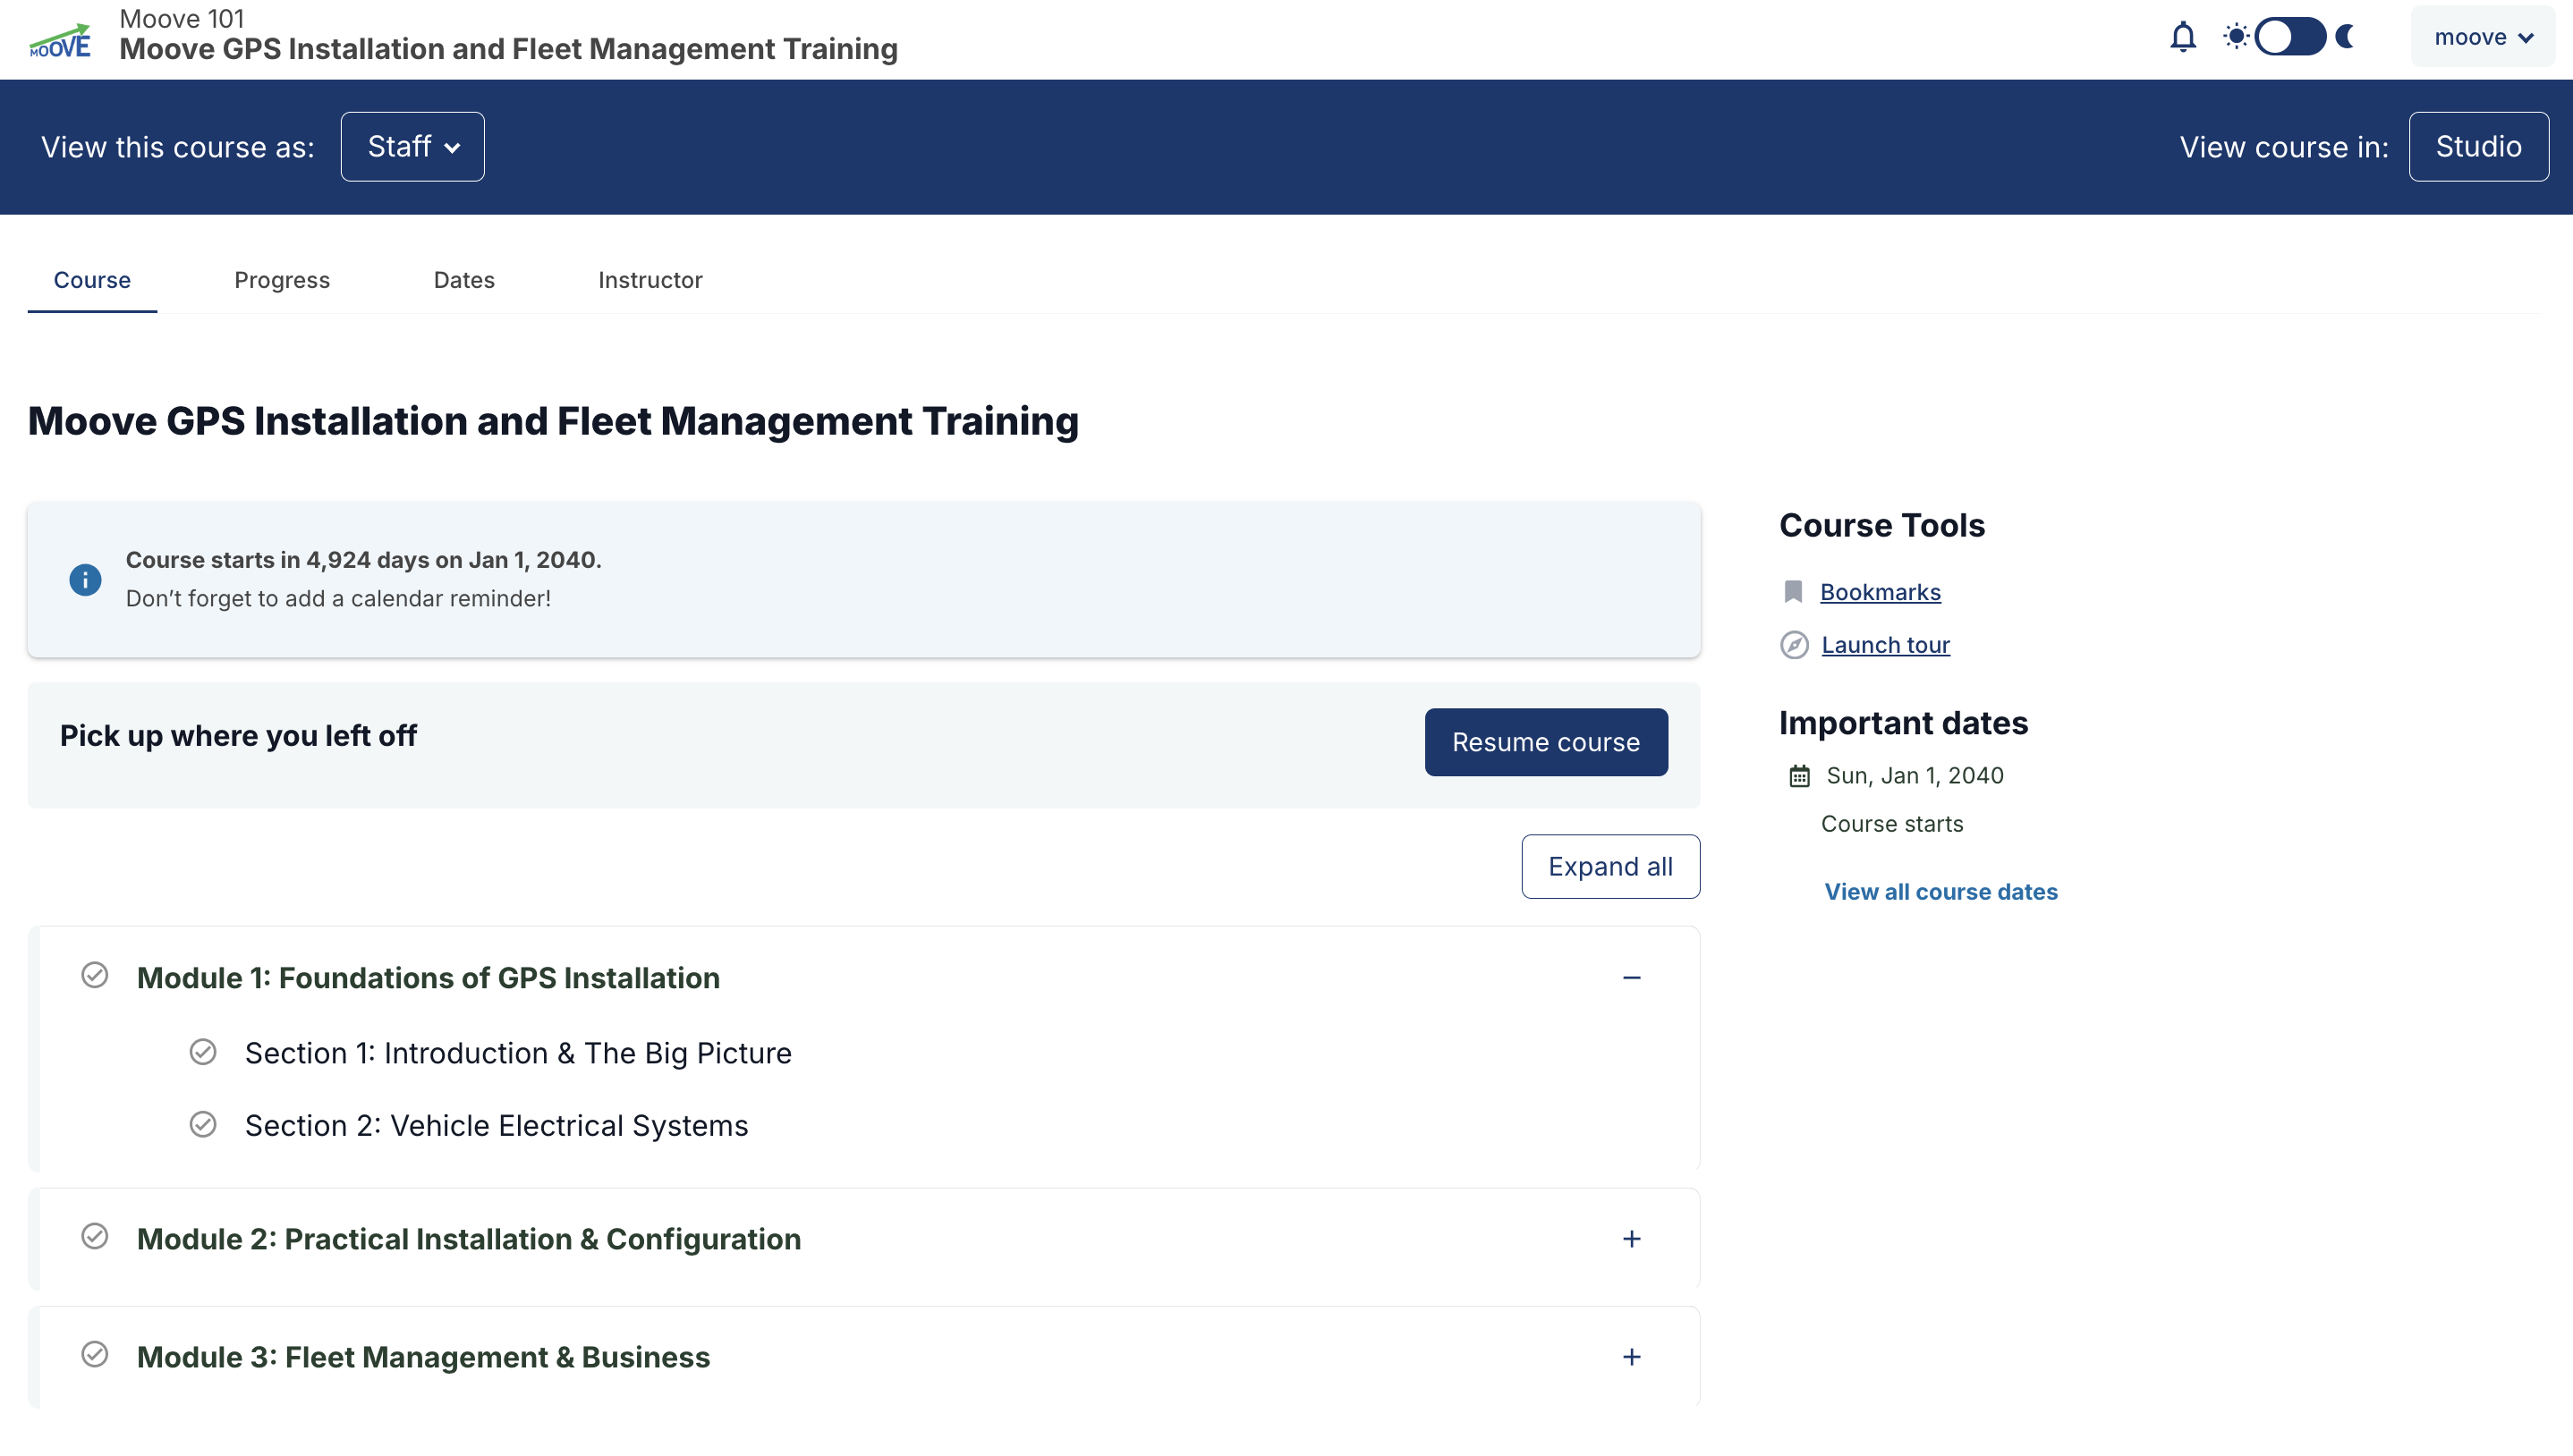
\includegraphics[width=\textwidth,height=0.6\textheight,keepaspectratio]{screenshots/enroll_course.png}
\caption{Course Enrollment}
\label{fig:enroll-course}
\end{figure}

\subsubsection{Open and Start a Course (UFR-OE-103-02)}
\begin{enumerate}
    \item From your dashboard, click the course card.
    \item Click \textbf{Start Course} or \textbf{Resume Course}.
    \item You will be taken to the first available content.
\end{enumerate}

\subsection{Course Prerequisites}

\subsubsection{Overview of Prerequisites (UFR-OE-104-01)}
\begin{itemize}
    \item Some courses have prerequisites: completion of another course or an entrance exam.
    \item Prerequisites are displayed on the course info page.
    \item You can view your completion status of prerequisites.
\end{itemize}

\subsubsection{Prerequisite Course (UFR-OE-104-02)}
\begin{enumerate}
    \item If a prerequisite course is required, complete it first.
    \item Once completed, the advanced course will become available.
\end{enumerate}

\subsubsection{Entrance Exam (UFR-OE-104-03)}
\begin{enumerate}
    \item If an entrance exam is required, you will be prompted to take it.
    \item The exam is typically a timed test.
    \item You must pass to gain access to the course.
\end{enumerate}

\subsection{Course Content Access}

\subsubsection{Troubleshoot Accessing Course Content (UFR-OE-105-01)}
\begin{itemize}
    \item If content is not accessible, check if it has a release date.
    \item Check if you have completed any prerequisites.
    \item Ensure you are enrolled in the course.
    \item Contact course staff if issues persist.
\end{itemize}

\subsubsection{Access an Archived Course (UFR-OE-105-02)}
\begin{enumerate}
    \item From your dashboard, click \textbf{Archived Courses}.
    \item Select the archived course you wish to view.
    \item Content is read-only; you cannot submit assignments.
\end{enumerate}

\subsubsection{View a Final Course Grade (UFR-OE-105-03)}
\begin{enumerate}
    \item Go to your course dashboard.
    \item Click \textbf{Grades} or \textbf{Progress}.
    \item Your final grade will be displayed at the top.
\end{enumerate}

\subsubsection{View Certificate Status (UFR-OE-105-04)}
\begin{enumerate}
    \item Go to your profile page.
    \item Click \textbf{Certificates}.
    \item You will see a list of courses and certificate status:
    \begin{itemize}
        \item \textbf{Eligible}: You can generate the certificate.
        \item \textbf{Available}: Certificate is ready to download.
        \item \textbf{Not Eligible}: You did not meet the passing criteria.
    \end{itemize}
\end{enumerate}

\begin{figure}[H]
\centering
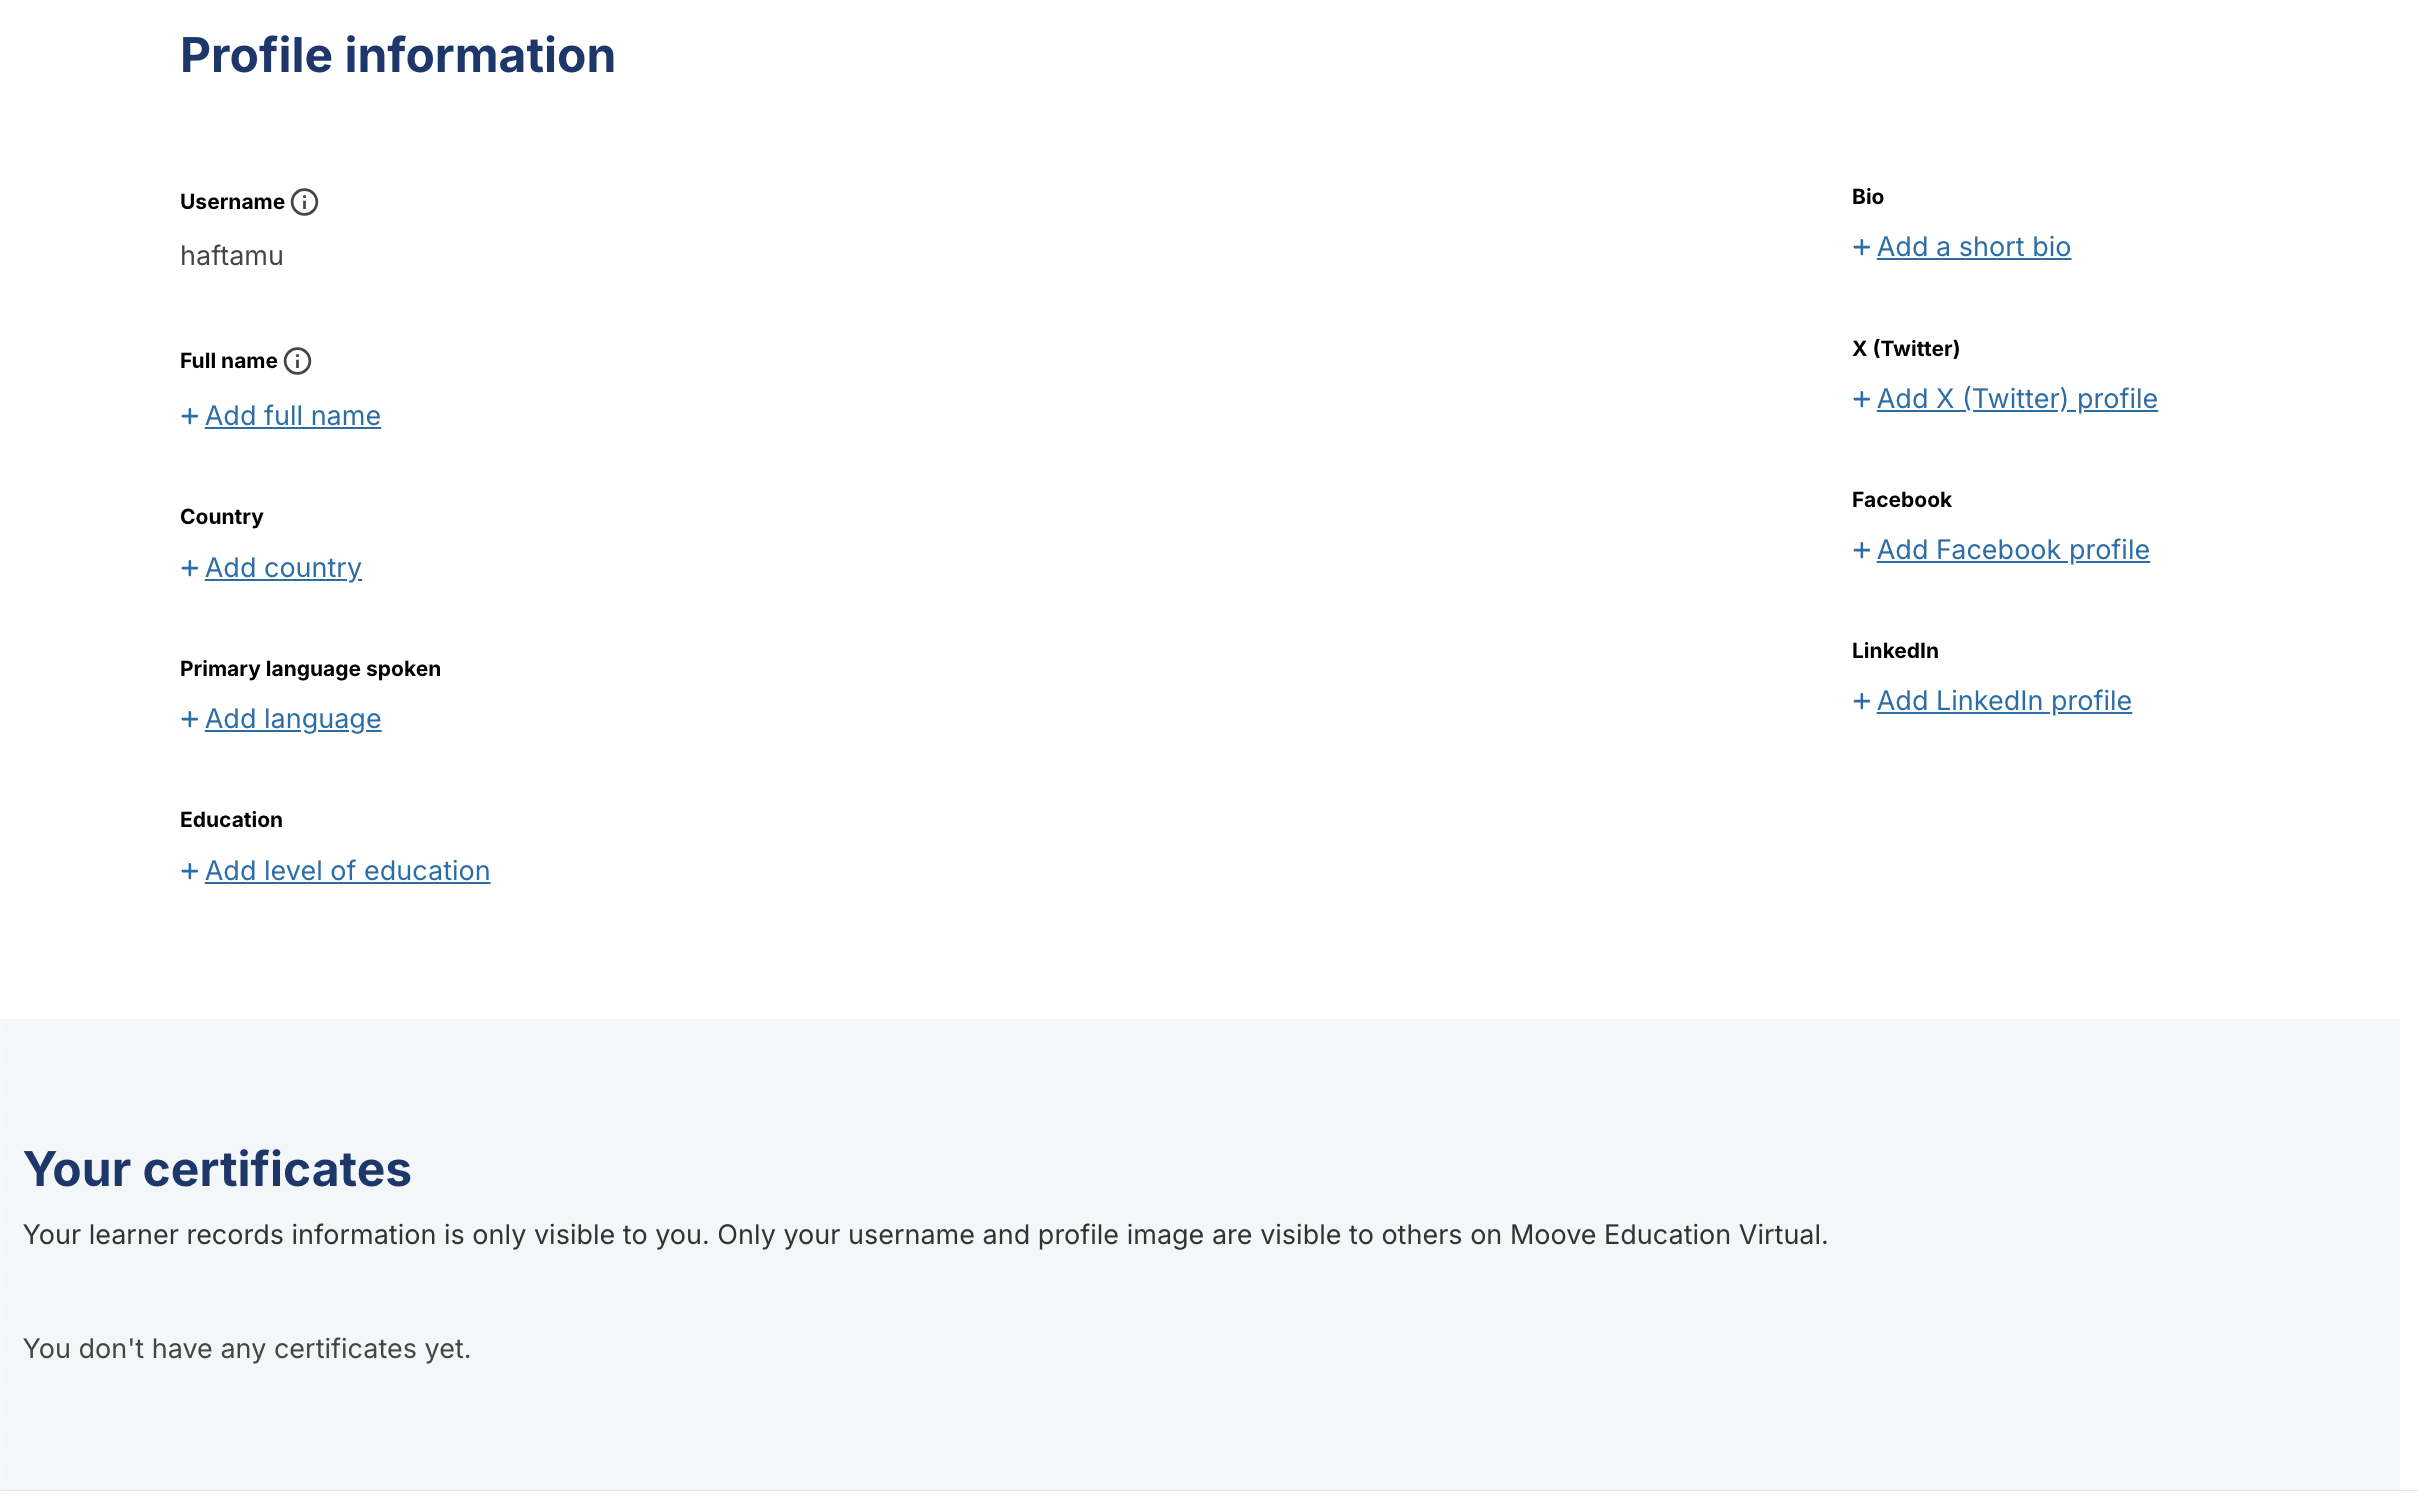
\includegraphics[width=\textwidth,height=0.6\textheight,keepaspectratio]{screenshots/certificate_status.png}
\caption{Certificate Status}
\label{fig:certificate-status}
\end{figure}

\subsection{Course Progress}

\subsubsection{Find a Course Start Date (UFR-OE-106-01)}
\begin{enumerate}
    \item Go to the course info page (before enrolling).
    \item The start date is displayed prominently.
    \item On the dashboard, the course card also shows the start date.
\end{enumerate}

\subsubsection{Start or Resume a Course (UFR-OE-106-02)}
\begin{enumerate}
    \item From your dashboard, click the course card.
    \item If not started, click \textbf{Start Course}.
    \item If already started, click \textbf{Resume Course}.
    \item The system will take you to your last visited content.
\end{enumerate}

\subsubsection{Progress Indicators (UFR-OE-106-03)}
\begin{itemize}
    \item Course cards on the dashboard show overall completion progress.
    \item Within a course, each section/subsection has a progress bar.
    \item Completed items are marked with a checkmark.
\end{itemize}

\subsubsection{The Progress Page (UFR-OE-106-04)}
\begin{enumerate}
    \item In a course, click \textbf{Progress} in the top navigation.
    \item You will see a detailed breakdown:
    \begin{itemize}
        \item Completion per section.
        \item Scores for each assignment.
        \item Overall course grade.
    \end{itemize}
\end{enumerate}

\begin{figure}[H]
\centering
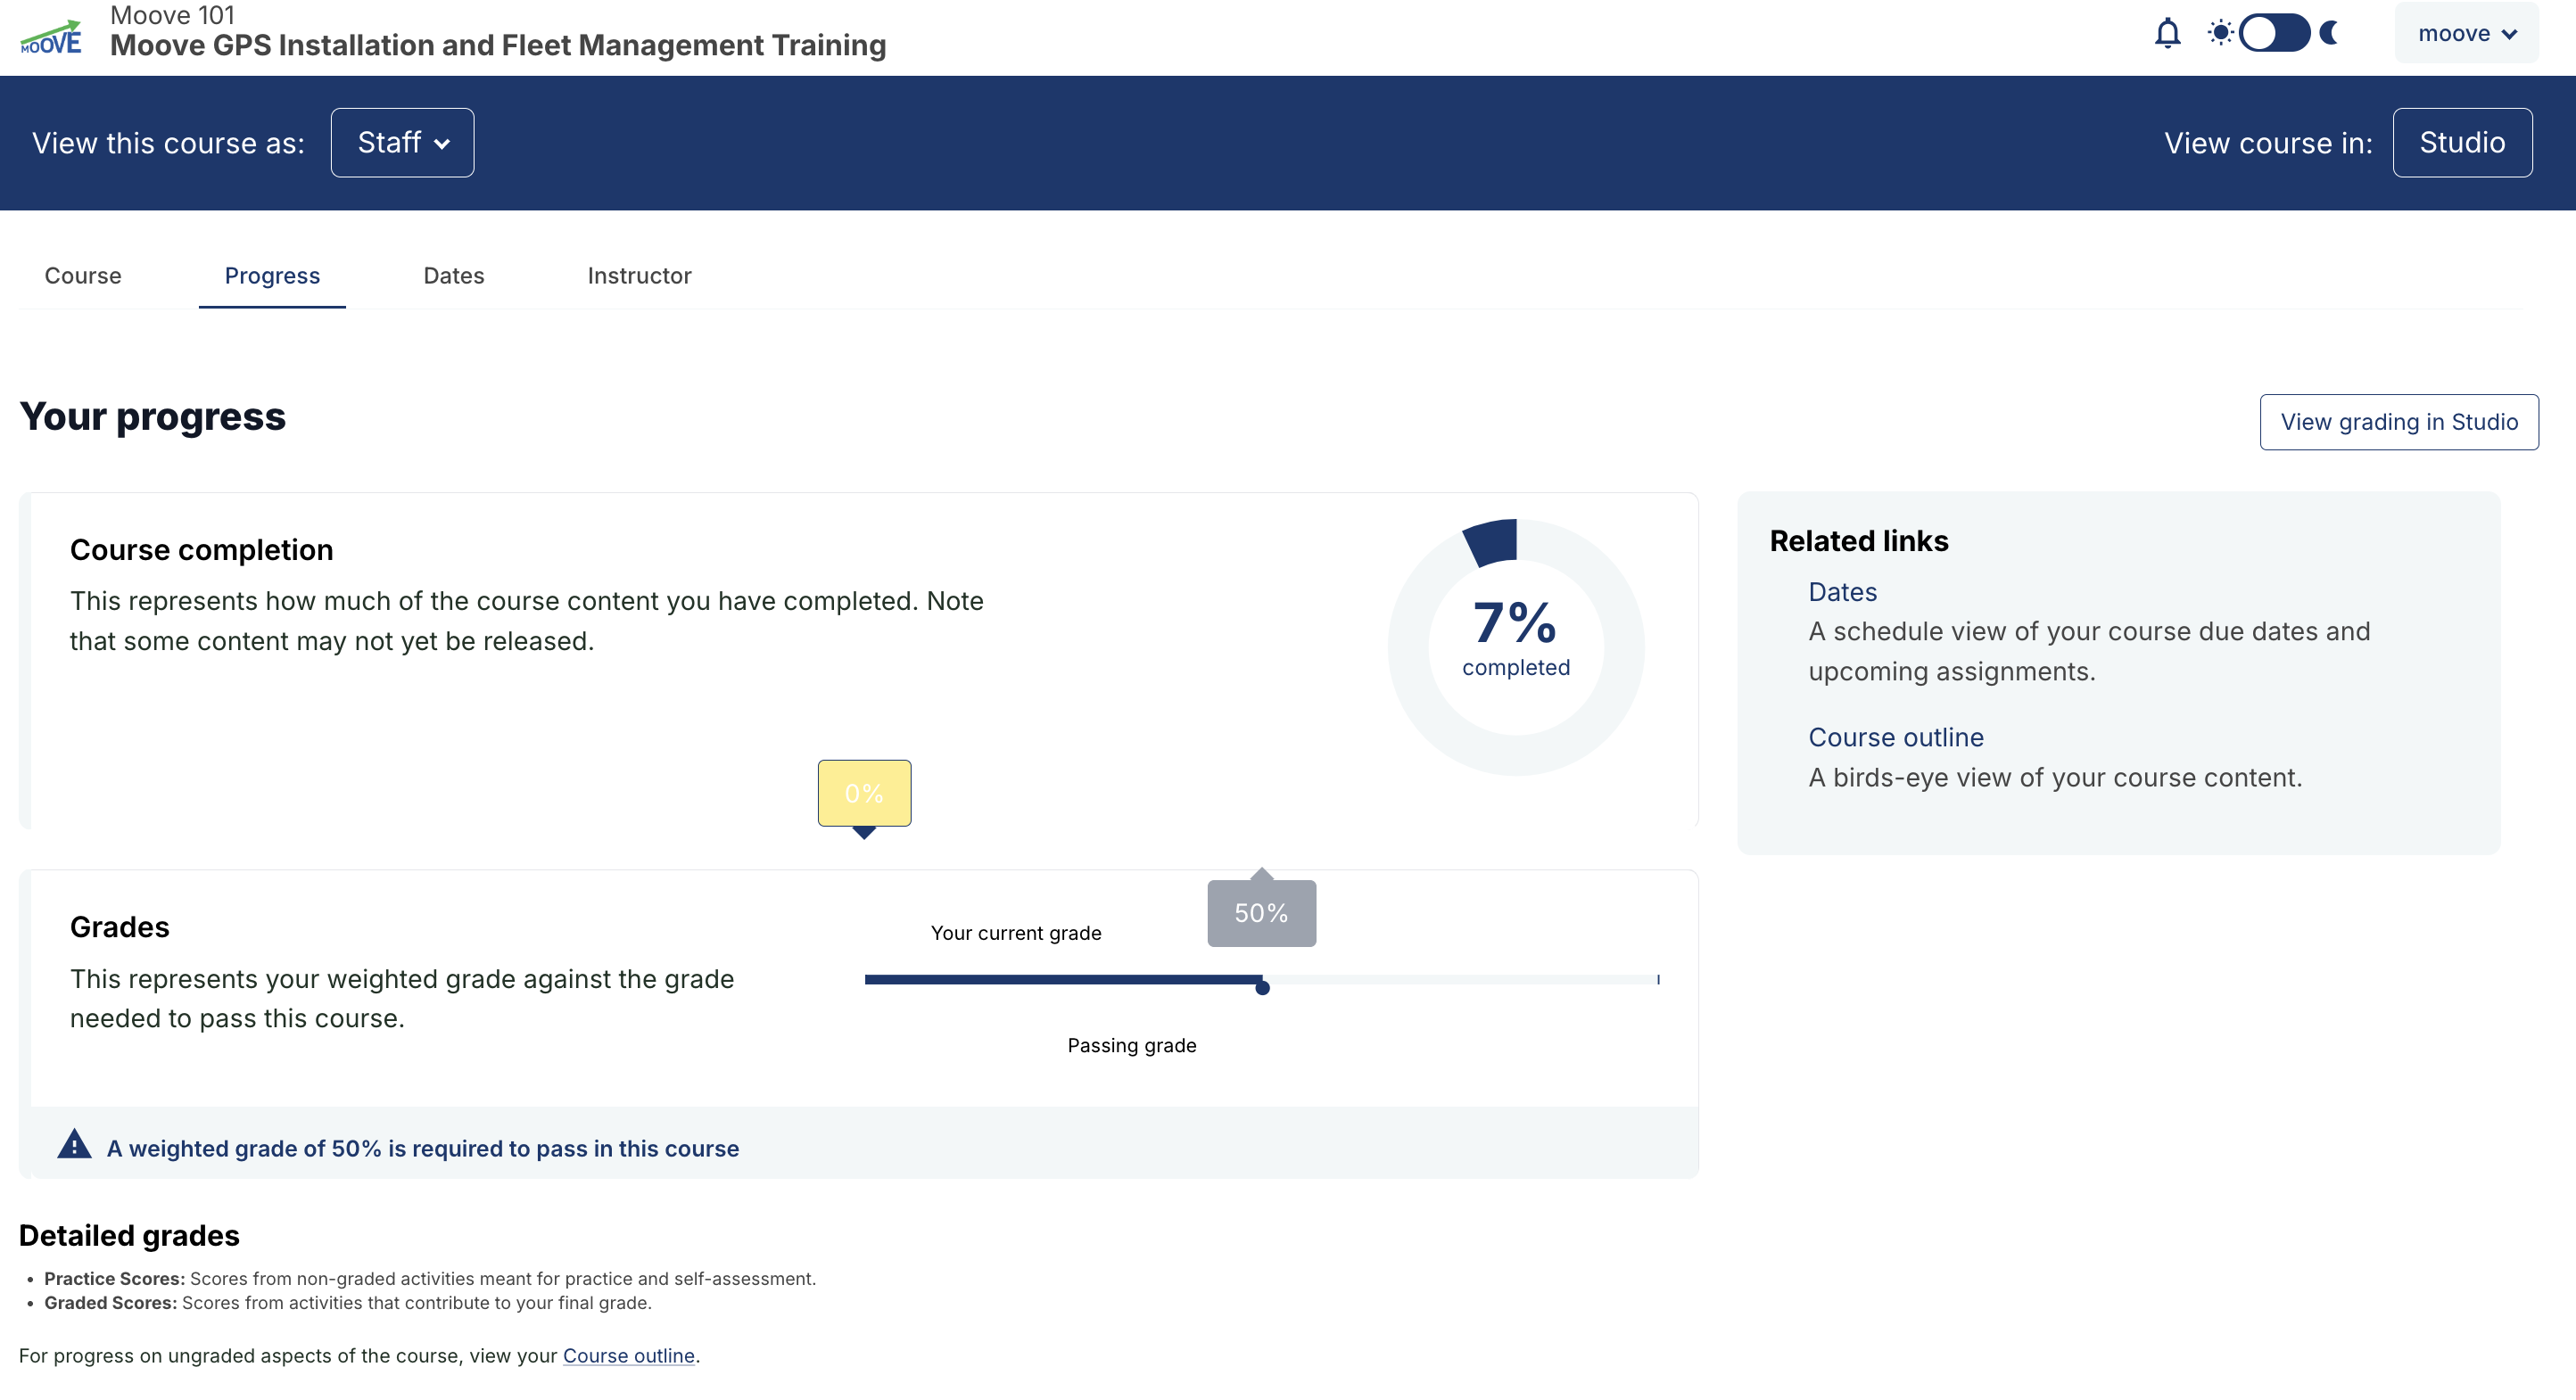
\includegraphics[width=\textwidth,height=0.6\textheight,keepaspectratio]{screenshots/progress_page.png}
\caption{Progress Page}
\label{fig:progress-page}
\end{figure}

\subsection{Certificates \& Badges}

\subsubsection{Accessing a Certificate (UFR-OE-107-01)}
\begin{enumerate}
    \item Go to your profile page.
    \item Click \textbf{Certificates}.
    \item Find the course with an \textbf{Available} certificate.
    \item Click \textbf{Download} or \textbf{Print}.
\end{enumerate}

\subsubsection{Viewing Earned Badges in Your Profile (UFR-OE-107-02)}
\begin{enumerate}
    \item Go to your profile page.
    \item Scroll down to the \textbf{Badges} section.
    \item Earned badges are displayed.
    \item Click a badge to view its details.
\end{enumerate}

\subsubsection{Sharing Badges on Mozilla Backpack (UFR-OE-107-03)}
\begin{enumerate}
    \item Click on a badge in your profile.
    \item Click \textbf{Share to Backpack}.
    \item Log in to your Mozilla Backpack account.
    \item The badge will be added to your backpack.
\end{enumerate}

\subsection{Watching Videos}

\subsubsection{Watching Videos on the Open edX Video Player (UFR-OE-108-01)}
\begin{enumerate}
    \item Navigate to a unit containing a video.
    \item The video player will appear.
    \item Controls include:
    \begin{itemize}
        \item Play/Pause.
        \item Volume slider.
        \item Speed control (0.5x, 1x, 1.25x, 1.5x, 2x).
        \item Full-screen toggle.
        \item Closed Captions (if transcripts are available).
    \end{itemize}
\end{enumerate}

\begin{figure}[H]
\centering
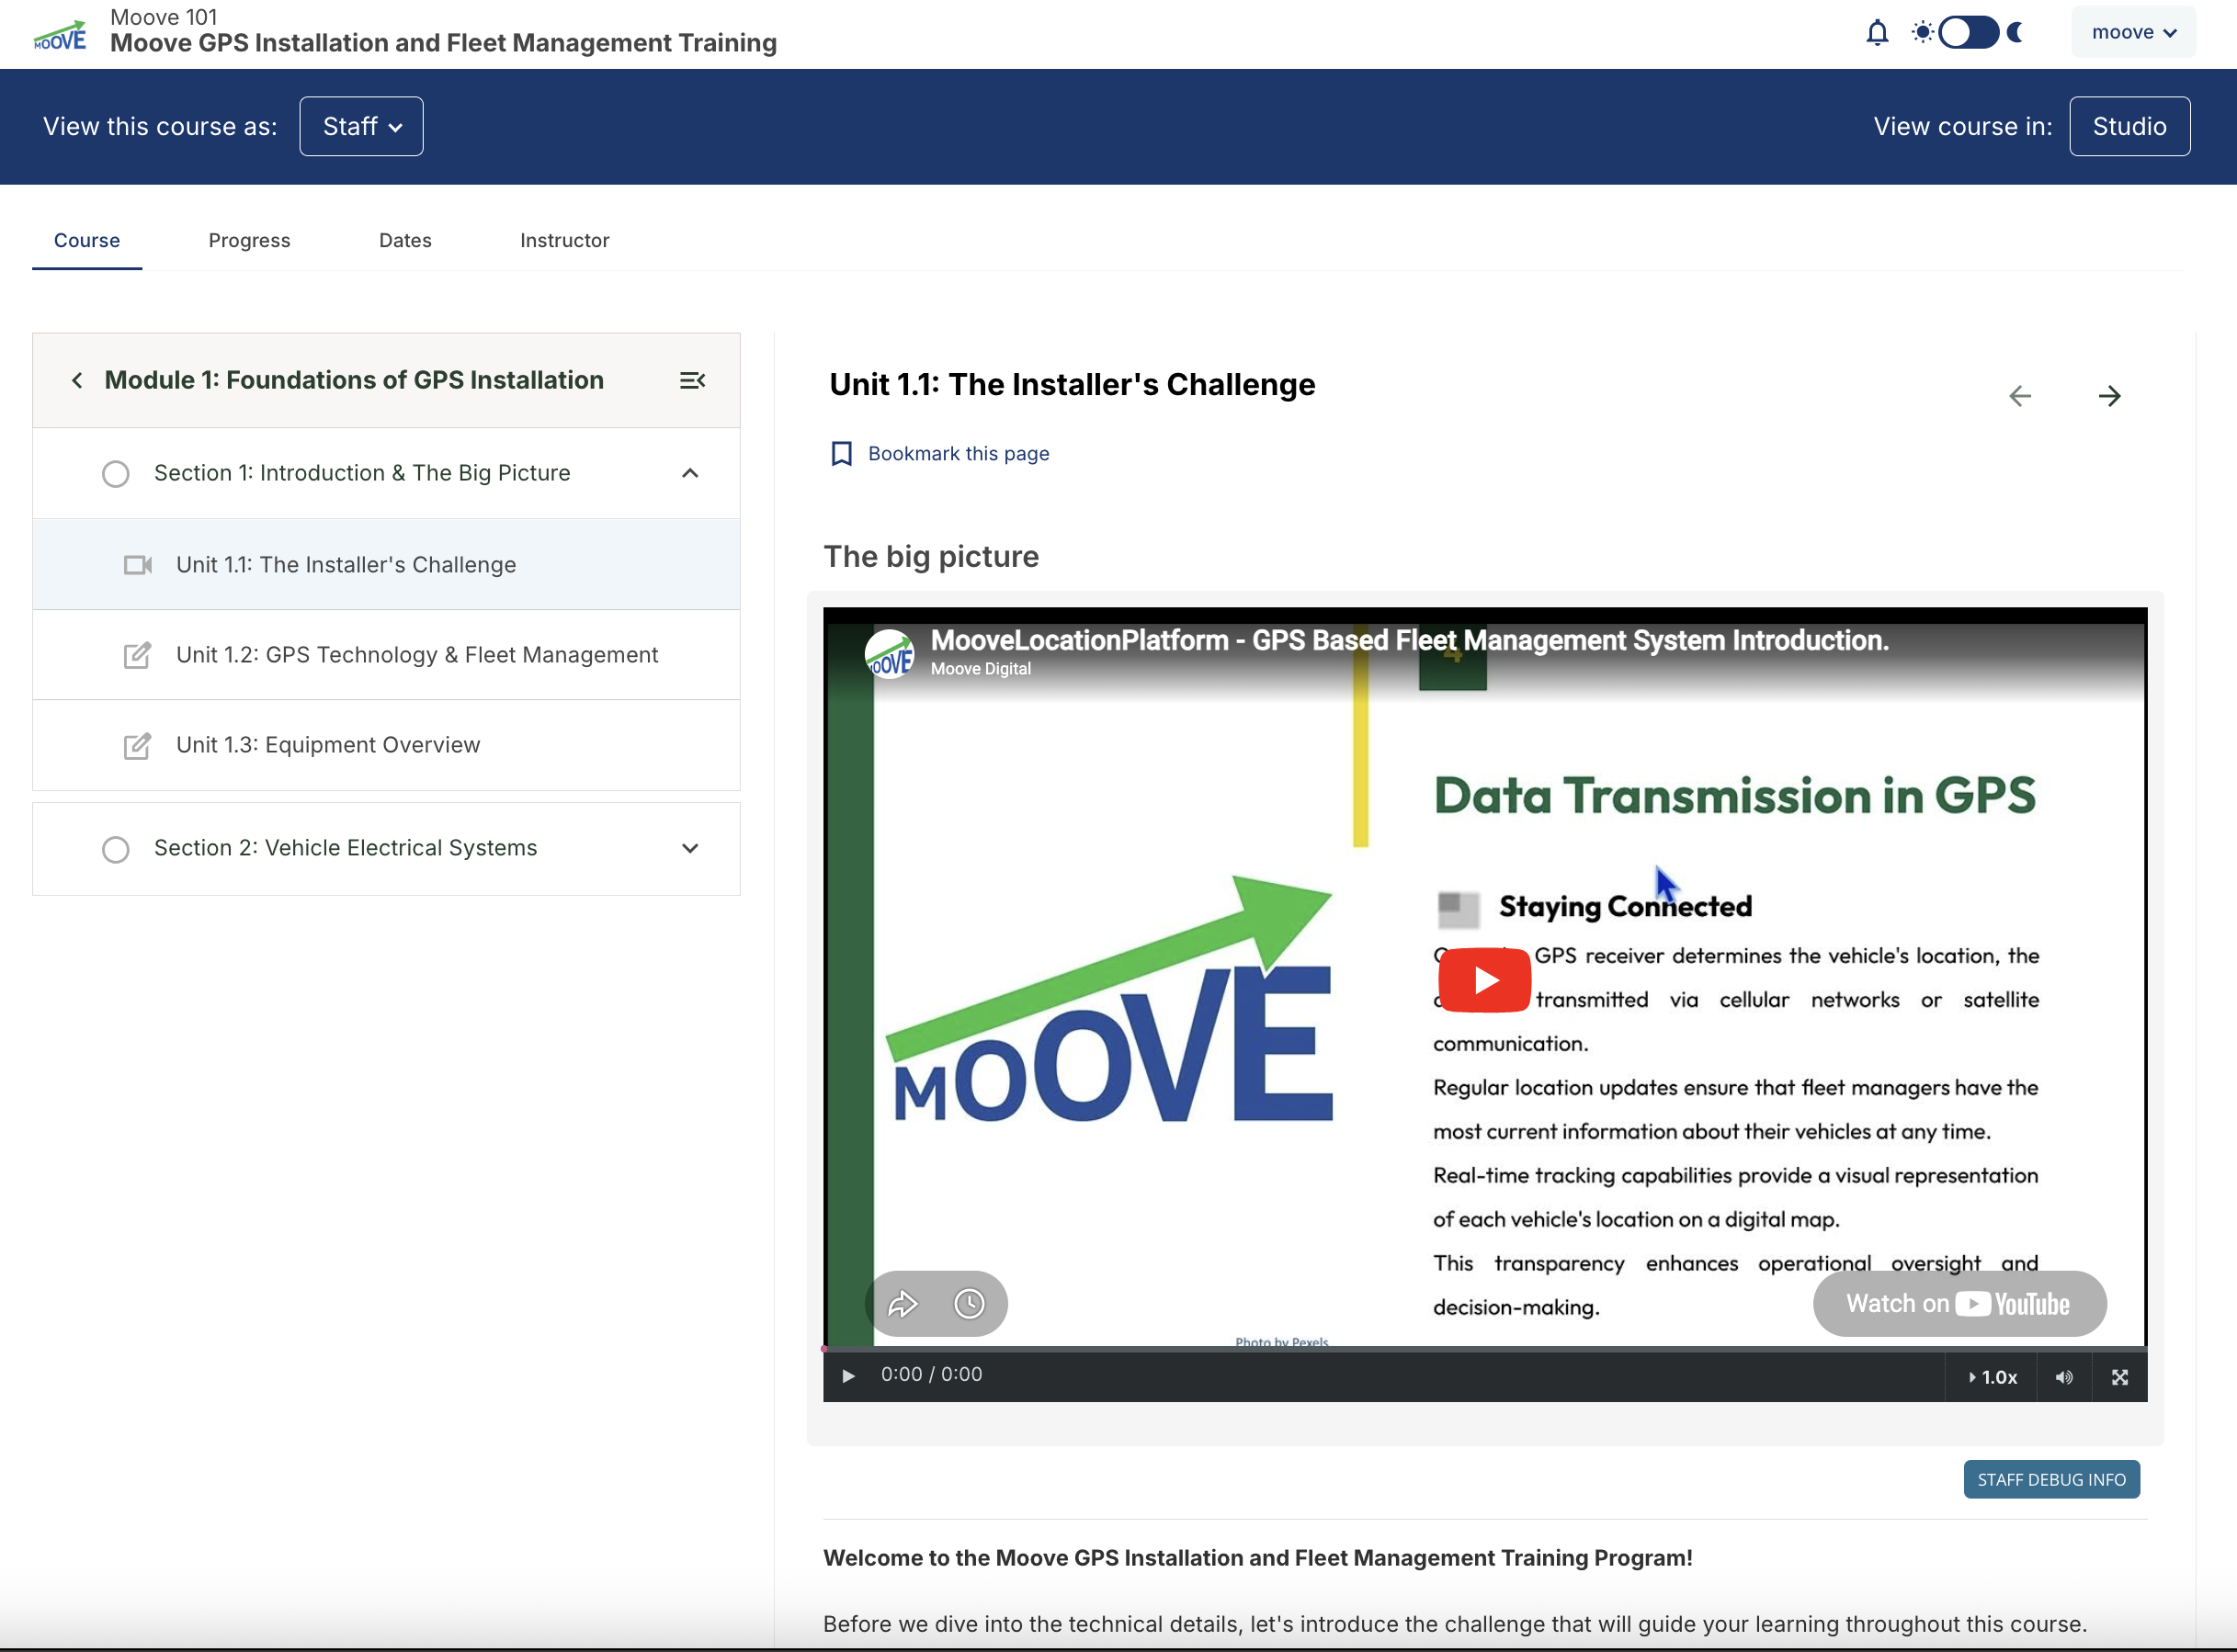
\includegraphics[width=\textwidth,height=0.6\textheight,keepaspectratio]{screenshots/video_player.png}
\caption{Video Player}
\label{fig:video-player}
\end{figure}

\subsection{Participating in Course Discussions}

\subsubsection{Getting Started with Discussions (UFR-OE-109-01)}
\begin{enumerate}
    \item In a course, click the \textbf{Discussions} tab in the top navigation.
    \item You will see all discussion threads and topics.
    \item Click on a thread to view and participate.
\end{enumerate}

\begin{figure}[H]
\centering
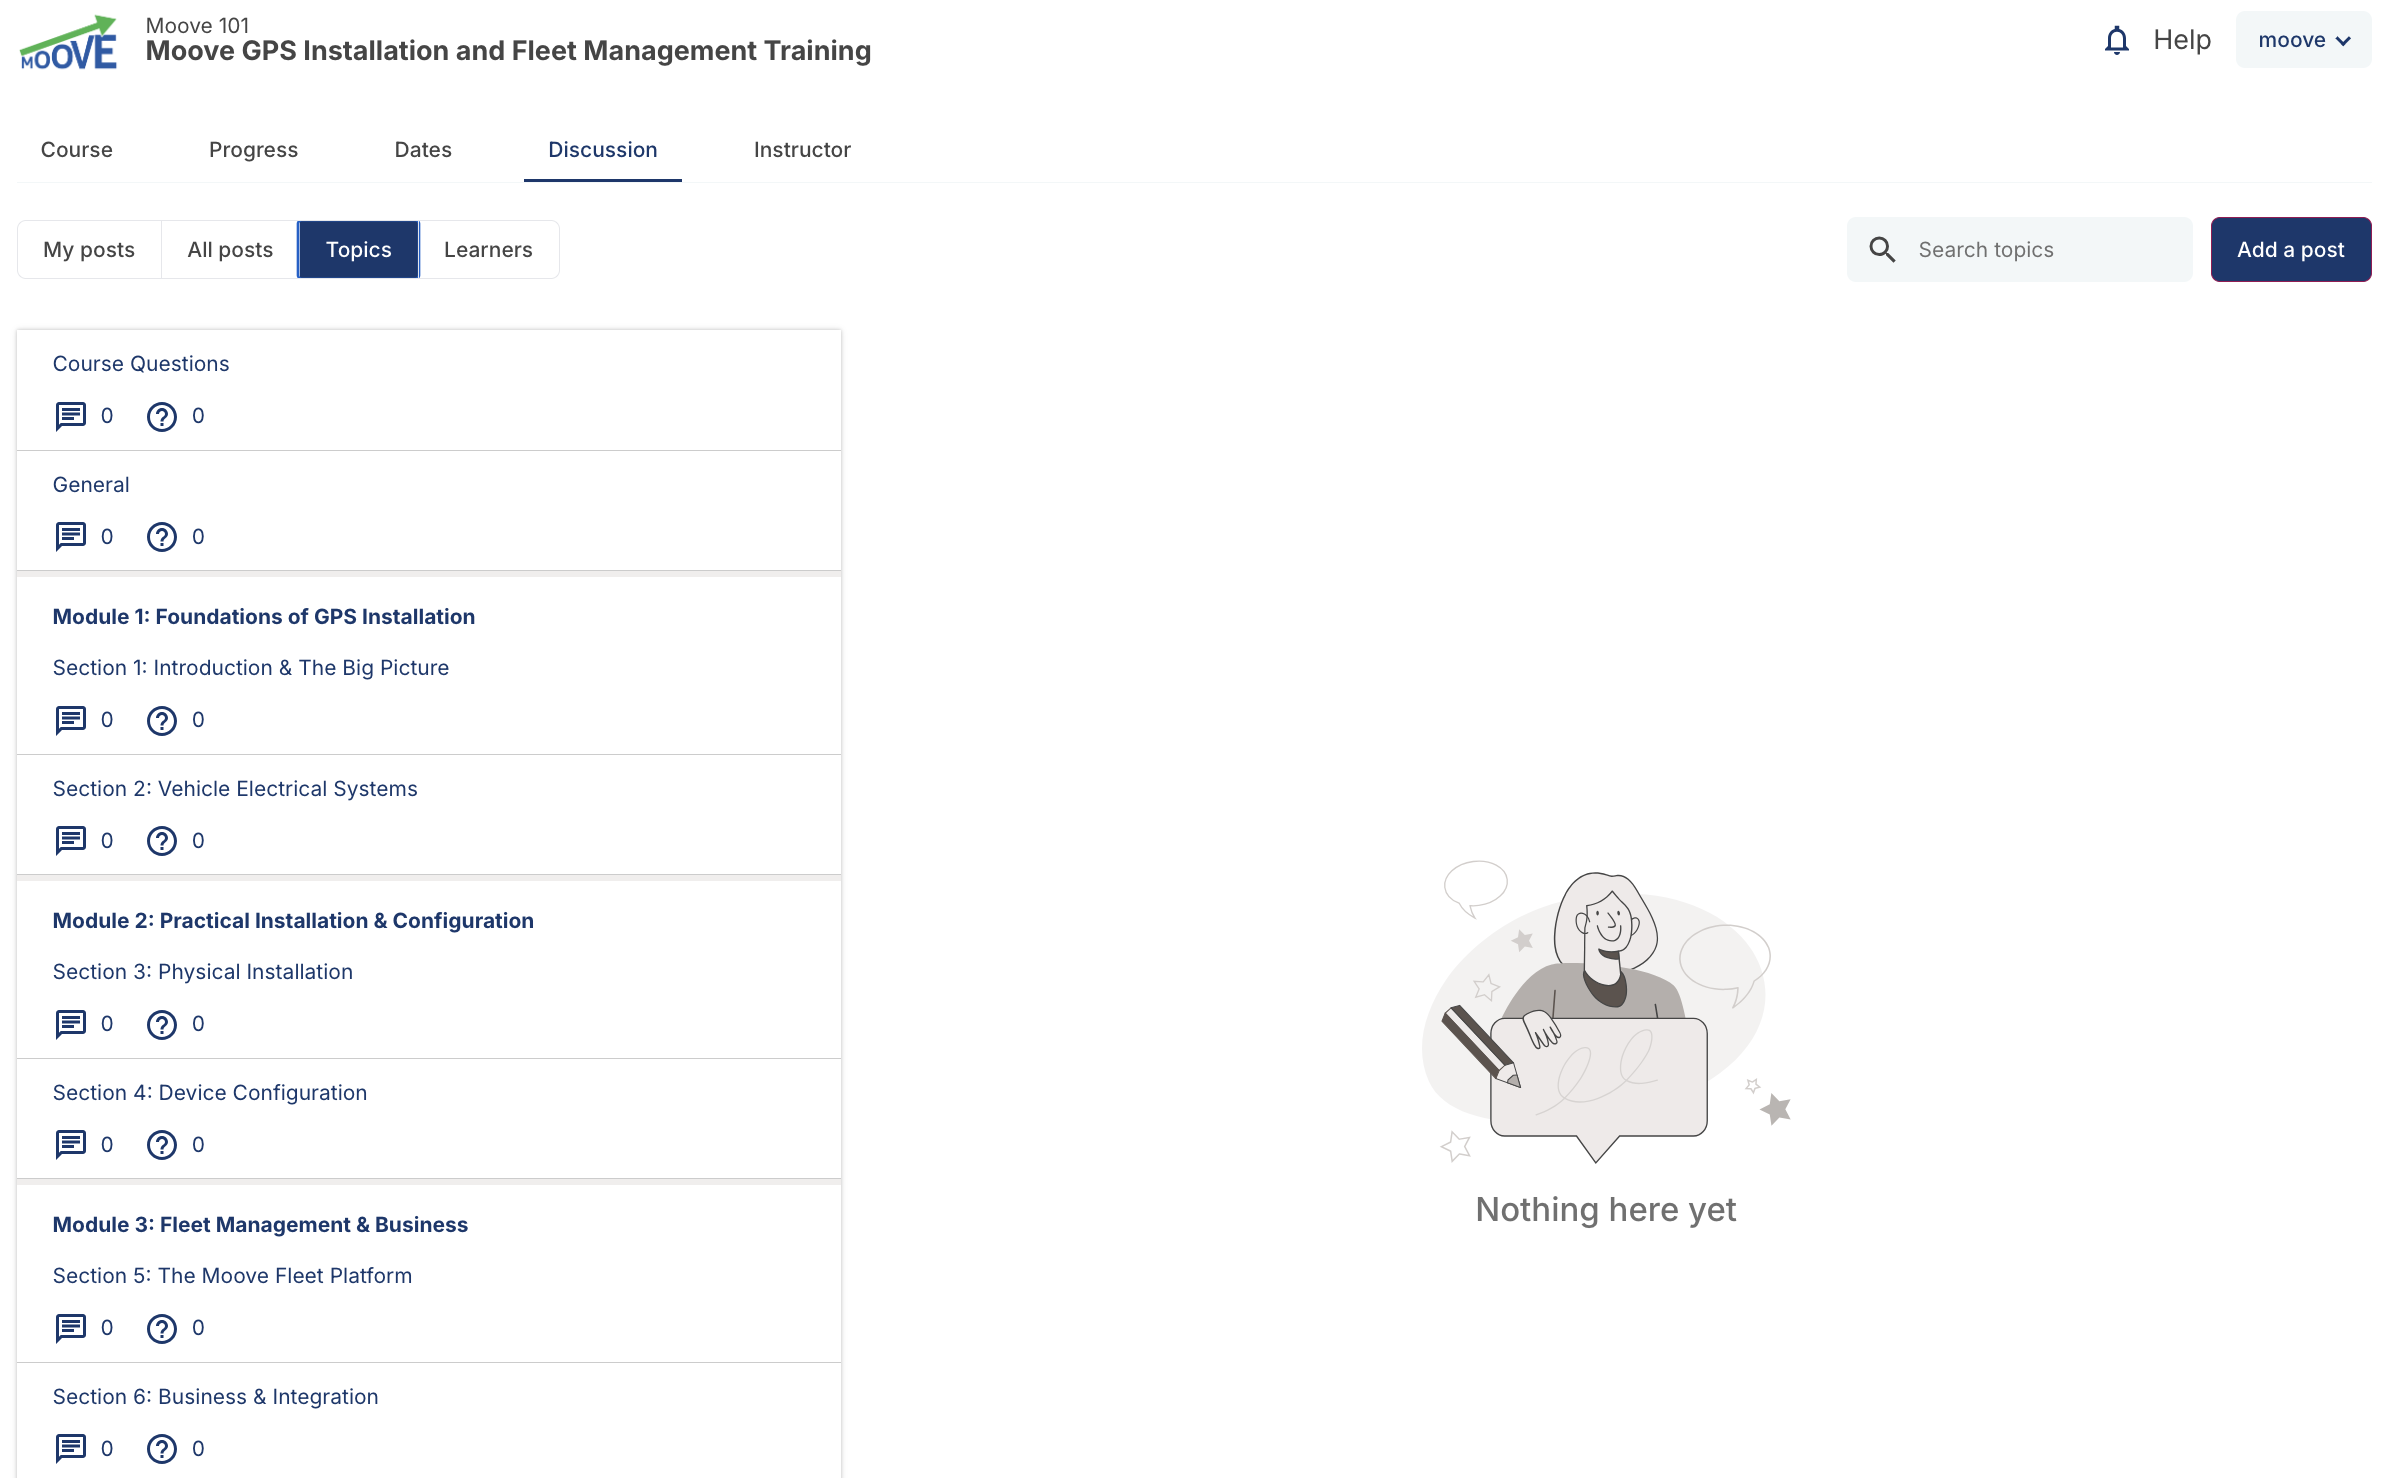
\includegraphics[width=\textwidth,height=0.6\textheight,keepaspectratio]{screenshots/discussions.png}
\caption{Discussions View}
\label{fig:discussions}
\end{figure}

\subsubsection{Finding and Following the Right Conversations (UFR-OE-109-02)}
\begin{enumerate}
    \item In the Discussions area, use the search bar to find topics.
    \item Filter by categories, tags, or recency.
    \item Click \textbf{Follow} on a thread to receive email notifications.
\end{enumerate}

\subsubsection{Taking Part in Discussions (UFR-OE-109-03)}
\begin{enumerate}
    \item To start a new thread: click \textbf{New Post}.
    \item Enter a title and content.
    \item Select a category/topic.
    \item Click \textbf{Post}.
    \item To reply: click \textbf{Reply} on a post or thread.
    \item Enter your response and click \textbf{Post}.
\end{enumerate}

\subsubsection{Staying Updated with Notifications (UFR-OE-109-04)}
\begin{itemize}
    \item You will receive email notifications for:
    \begin{itemize}
        \item Replies to threads you follow.
        \item Direct replies to your posts.
        \item Course announcements.
    \end{itemize}
    \item Configure notification preferences from your profile.
\end{itemize}

\subsection{Completing Different Types of Assignments}

\subsubsection{Completing Mathematical and Scientific Assignments (UFR-OE-110-01)}
\begin{itemize}
    \item Use LaTeX notation for math (e.g., \texttt{\$E=mc\textasciicircum 2\$}).
    \item Supported in text responses and essay fields.
\end{itemize}

\subsubsection{Taking a Timed Exam (UFR-OE-110-02)}
\begin{enumerate}
    \item Start the exam by clicking \textbf{Start}.
    \item A timer will begin counting down.
    \item You must complete the exam before the time expires.
    \item At expiration, the exam will auto-submit.
\end{enumerate}

\subsubsection{Proctored Exams (UFR-OE-110-03)}
\begin{enumerate}
    \item Proctored exams require identity verification.
    \item You may need to install a proctoring software extension.
    \item Follow the instructions to complete identity verification.
    \item Take the exam as usual; the proctoring software monitors the session.
\end{enumerate}

\subsubsection{Explaining Multiple Choice Answers (UFR-OE-110-04)}
\begin{enumerate}
    \item For some multiple-choice questions, an explanation field is provided.
    \item Select your answer.
    \item Optionally, enter a brief explanation of your reasoning.
    \item Click \textbf{Submit}.
\end{enumerate}

\subsubsection{Completing Essay Assignments (UFR-OE-110-05)}
\begin{enumerate}
    \item Open the assignment unit.
    \item Read the prompt.
    \item Write your essay in the text editor (supports formatting, images, etc.).
    \item Click \textbf{Submit} to submit your assignment.
\end{enumerate}

\subsubsection{The Steps in an Open Response Assessment (UFR-OE-110-06)}
\begin{enumerate}
    \item \textbf{Submission}: Submit your response.
    \item \textbf{Self-Assessment}: Evaluate your own work using the rubric.
    \item \textbf{Peer Assessment}: Review submissions from other learners.
    \item \textbf{Staff Assessment}: Instructor provides a final grade.
\end{enumerate}

\subsubsection{How Grading Is Done in Open Response Assessments (UFR-OE-110-07)}
\begin{itemize}
    \item Each rubric criterion has a score level.
    \item Peer assessors score each criterion.
    \item The final score is an average (or median) of peer scores.
    \item Staff assessment overrides peer scores.
\end{itemize}

\subsubsection{Completing an Open Response Assessment (UFR-OE-110-08)}
\begin{enumerate}
    \item Go to the assignment unit.
    \item Click \textbf{Submit Response}.
    \item Write your response.
    \item Click \textbf{Submit}.
    \item After submission, proceed to self-assessment and peer assessment.
\end{enumerate}

\subsubsection{Receive Your Score and Provide Feedback (UFR-OE-110-09)}
\begin{enumerate}
    \item After all assessments are complete, your score will appear.
    \item You will also receive feedback from peers and staff.
    \item Provide feedback on the assessment experience (optional).
\end{enumerate}

\subsubsection{How Peer Assessment Scores Are Calculated (UFR-OE-110-10)}
\begin{itemize}
    \item Each learner reviews 3-5 peer submissions.
    \item Scores are combined (average, median, or adjusted).
    \item The system ensures fairness by detecting outliers.
\end{itemize}

\subsubsection{Canceled Responses (UFR-OE-110-11)}
\begin{enumerate}
    \item You may cancel your submission before the assessment phase.
    \item Go to the assignment unit.
    \item Click \textbf{Cancel Submission}.
    \item You can resubmit later (if allowed).
\end{enumerate}

\subsection{Working on Team Projects and Activities}

\subsubsection{About Teams and Topics (UFR-OE-111-01)}
\begin{itemize}
    \item Teams are groups of learners working together on a project.
    \item Each course can define topics and allow team creation.
\end{itemize}

\subsubsection{Search for a Team (UFR-OE-111-02)}
\begin{enumerate}
    \item Go to the course \textbf{Teams} page.
    \item Use the search bar to find teams by name or topic.
    \item View team details and members.
\end{enumerate}

\subsubsection{Join a Team (UFR-OE-111-03)}
\begin{enumerate}
    \item Find a team you want to join.
    \item Click \textbf{Join Team}.
    \item The team owner will be notified (or auto-approved if open enrollment).
\end{enumerate}

\subsubsection{Leave a Team (UFR-OE-111-04)}
\begin{enumerate}
    \item Go to the team page.
    \item Click \textbf{Leave Team}.
    \item Confirm your departure.
\end{enumerate}

\subsubsection{Create a Team (UFR-OE-111-05)}
\begin{enumerate}
    \item Go to the course \textbf{Teams} page.
    \item Click \textbf{Create Team}.
    \item Enter a name, description, and topic.
    \item Set enrollment type (Open or Request to Join).
    \item Click \textbf{Create}.
\end{enumerate}

\subsubsection{Participating in Team Discussions (UFR-OE-111-06)}
\begin{enumerate}
    \item Team discussions are available within the team page.
    \item Team members can start threads and reply.
    \item These discussions are private to the team.
\end{enumerate}

\subsection{Searching the Course}

\subsubsection{Overview of Search (UFR-OE-112-01)}
\begin{itemize}
    \item Search is powered by Meilisearch.
    \item It indexes course content, discussions, and resources.
    \item Search results are fast and relevant.
\end{itemize}

\subsubsection{Search a Single Course (UFR-OE-112-02)}
\begin{enumerate}
    \item In a course, look for the search bar (usually in the sidebar or top nav).
    \item Enter your query.
    \item Results will show relevant content from within the course.
\end{enumerate}

\subsubsection{Search All Your Courses (UFR-OE-112-03)}
\begin{enumerate}
    \item On the dashboard, enter your query in the global search bar.
    \item Results will include content from all your enrolled courses.
\end{enumerate}

\subsection{Bookmarking Course Content}

\subsubsection{Add or Remove a Bookmark (UFR-OE-113-01)}
\begin{enumerate}
    \item In a course, go to any content unit.
    \item Click the \textbf{Bookmark} icon (bookmark outline).
    \item The icon will fill (bookmark added).
    \item Click again to remove the bookmark.
\end{enumerate}

\subsubsection{View Your Bookmarks (UFR-OE-113-02)}
\begin{enumerate}
    \item Click your avatar in the top-right corner.
    \item Select \textbf{Bookmarks}.
    \item You will see a list of all bookmarked content.
    \item Click any item to navigate directly.
\end{enumerate}

\begin{figure}[H]
\centering
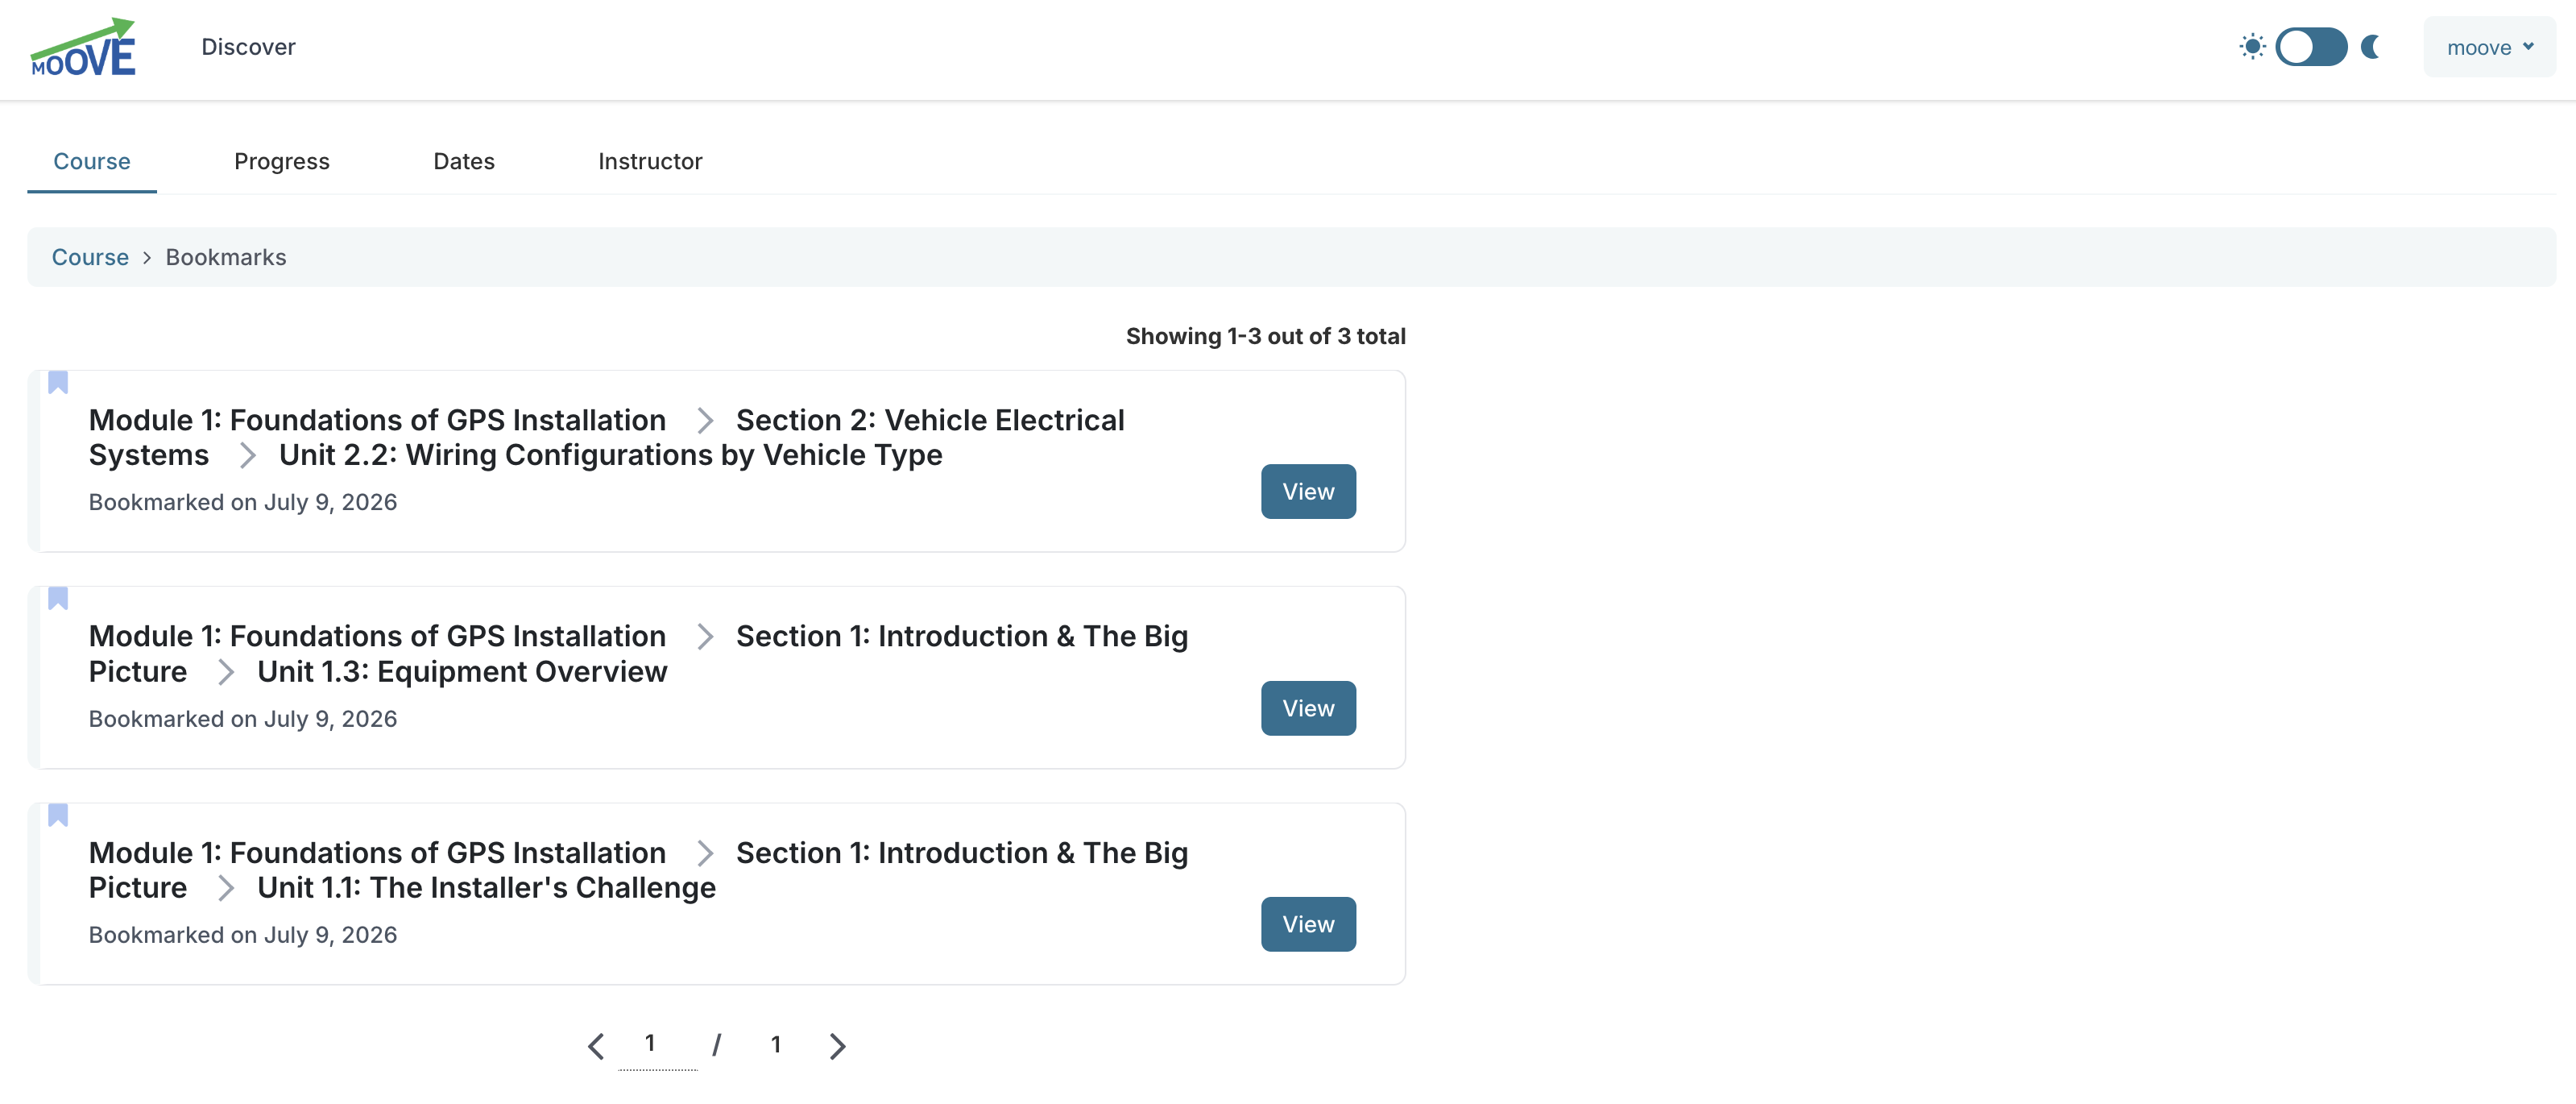
\includegraphics[width=\textwidth,height=0.6\textheight,keepaspectratio]{screenshots/bookmarks.png}
\caption{Bookmarks View}
\label{fig:bookmarks}
\end{figure}

\subsection{Notifications \& Preferences}

\subsubsection{Where Notifications Appear (UFR-OE-114-01)}
\begin{itemize}
    \item Notifications appear in three places:
    \begin{itemize}
        \item \textbf{In-app}: Bell icon in the top bar.
        \item \textbf{Email}: Sent to your registered email address.
        \item \textbf{Dashboard}: Recent activity alerts.
    \end{itemize}
\end{itemize}

\subsubsection{Activity Types (UFR-OE-114-02)}
\begin{itemize}
    \item Discussion replies on threads you follow.
    \item Assignment due dates and deadlines.
    \item Course announcements and updates.
    \item Submission feedback and grades.
\end{itemize}

\subsubsection{Managing Preferences (UFR-OE-114-03)}
\begin{enumerate}
    \item Click your avatar in the top-right corner.
    \item Select \textbf{Settings} or \textbf{Preferences}.
    \item Choose which notifications to receive:
    \begin{itemize}
        \item Email notifications.
        \item In-app notifications.
        \item Frequency (Instant, Daily Digest, Weekly).
    \end{itemize}
    \item Click \textbf{Save}.
\end{enumerate}

\subsubsection{Notifications Expiry (UFR-OE-114-04)}
\begin{itemize}
    \item Notifications expire after 30 days.
    \item Expired notifications are automatically archived.
    \item You can still view archived notifications in your profile.
\end{itemize}

\subsection{Using the Course Wiki}

\subsubsection{View Live Course (UFR-OE-115-01)}
\begin{enumerate}
    \item If your course has a wiki, it appears in the course navigation.
    \item Click the \textbf{Wiki} tab.
    \item You can view and edit wiki pages (if permissions allow).
\end{enumerate}

\subsubsection{View Live Course (UFR-OE-115-02)}
\begin{enumerate}
    \item The live course is the published version of the course.
    \item Content that has been published and released is visible.
    \item In-progress or draft content is hidden from learners.
\end{enumerate}

% ---------------------------------------------------------------------
% NEW SECURITY AND PRIVACY SECTION
% ---------------------------------------------------------------------
\section{Security and Privacy (Mandatory)}
This section outlines the security responsibilities of all users, in line with INSA regulations and the organisation’s security policy.

\subsection{Password Management}
\begin{itemize}
    \item Use a strong, unique password (at least 12 characters, mix of uppercase, lowercase, numbers, and special characters).
    \item Never share your password with anyone.
    \item Change your password immediately if you suspect it has been compromised.
    \item Enable two‑factor authentication (if available) for your account.
\end{itemize}

\subsection{Protecting Personal Information}
\begin{itemize}
    \item Be cautious about the personal information you share in your profile and in discussions.
    \item Do not post sensitive information (e.g., phone numbers, addresses) in public forums.
    \item Review and adjust your privacy settings to control who can see your profile.
\end{itemize}

\subsection{Recognising Phishing and Suspicious Activities}
\begin{itemize}
    \item Do not click on links or open attachments from unknown senders.
    \item Be wary of emails that ask for your password or personal details.
    \item Report any suspicious emails or activity to the platform administrators immediately.
\end{itemize}

\subsection{Secure Use of the Platform}
\begin{itemize}
    \item Always log out after using the platform, especially on shared devices.
    \item Keep your browser and operating system up to date with the latest security patches.
    \item Use only official, approved browser extensions.
    \item Do not share your session or cookies with others.
\end{itemize}

\subsection{Reporting Security Incidents}
\begin{itemize}
    \item If you suspect a security breach, unauthorised access, or any vulnerability, report it immediately to the IT Security team at \texttt{security@educationvirtual.net}.
    \item Include as many details as possible (time, description, screenshots) to facilitate investigation.
\end{itemize}

\subsection{Compliance and Consequences}
All users are required to comply with the platform’s security policies and Ethiopian cyber laws (Computer Crime Proclamation No. 958/2016). Violations may result in disciplinary action, including account suspension or legal proceedings.

For more detailed security information, refer to the \textit{Security Architecture \& Threat Model} document available to authorised personnel.

\section{Troubleshooting}
\begin{itemize}
    \item \textbf{Cannot log in}: Check your email/password; reset password if needed.
    \item \textbf{Course not visible}: Ensure the course is published and you are enrolled.
    \item \textbf{Video not playing}: Check browser compatibility; try Chrome or Firefox.
    \item \textbf{Assignment not accessible}: Check deadlines and prerequisites.
    \item \textbf{Discussion not visible}: Ensure the course has discussions enabled.
    \item \textbf{Certificate not available}: Check if you passed the course and the certificate is generated.
    \item \textbf{Suspicious activity}: Immediately contact security@educationvirtual.net.
\end{itemize}

\section{References}
\begin{itemize}
    \item \textit{Security Architecture \& Threat Model – Moove Education Platform} (Security\_OpenEdX.tex)
    \item FDRE Computer Crime Proclamation No. 958/2016
    \item CMCSRS v2.0
\end{itemize}

% === LICENSE ATTRIBUTION ===
\newpage
\section*{Apache License 2.0 Attribution}
This product includes software developed by the \textbf{Open edX Project} (\url{https://open.edx.org/}) licensed under the Apache License, Version 2.0 (\url{http://www.apache.org/licenses/LICENSE-2.0}).

\textit{Moove Education Platform is a derivative work of Open edX. No modifications have been made to the original license terms. A copy of the full license text is available in the root of the source repository and in Appendix A of this document.}

% === OPTIONAL: Include full license in appendix ===
\appendix
\section{Full Apache License 2.0 Text}
\input{../common/license}

\end{document}
\end{document}